\documentclass[a4paper,11pt]{report}
\usepackage[utf8]{inputenc}
\usepackage[pdftex]{graphicx}
\usepackage{pdfpages}
\usepackage[pdftex]{graphicx}
\usepackage{fouriernc}
\usepackage[T1]{fontenc}
\usepackage{fancyhdr}
\usepackage{booktabs}	
\usepackage{multirow}
\usepackage{float}
\usepackage{caption}
\usepackage{subcaption}
\usepackage{listings}
\usepackage{titlesec} 
\usepackage{parskip}
\usepackage{url}
\usepackage{xcolor}
\usepackage{longtable}
\usepackage{tikz}
\usepackage{graphicx}
\usepackage[margin=1in]{geometry}
\usepackage[toc,page]{appendix}
\usepackage{float}
\usepackage{mathrsfs,amsmath,amssymb}   %The amsmath package is included for \xrightarrow
\usepackage[figurename=Fig.]{caption}
\usepackage{hyperref}
\hypersetup{
    colorlinks,
    citecolor=black,
    filecolor=black,
    linkcolor=black,
    urlcolor=black
}

\usepackage{sectsty}
\partfont{\large}

\usepackage{etoolbox}
\patchcmd{\abstract}{\titlepage}{\clearpage}{}{}
\patchcmd{\andabstract}{\endtitlepage}{\clearpage}{}{}


%\addtolength{\oddsidemargin}{-.5in}
%\addtolength{\evensidemargin}{-.5in}
%\addtolength{\textwidth}{1.75in}

%\addtolength{\topmargin}{-.875in}
%\addtolength{\textheight}{1.75in}



\usepackage[acronym]{glossaries}
\makeglossaries
% abbreviations:
\newacronym{hpc}{HPC}{High Performance Computing}
\newacronym{gcm}{GCM}{Global Circulation Model}
\newacronym{fft}{FFT}{Fast Fourier Transform}
\newacronym{fftw}{FFTW}{Fastest Fourier Transform in the West}
\newacronym{nag}{NAG}{Numerical Algorithms Group}
\newacronym{mpi}{MPI}{Message Passing Interface}
\newacronym{mpp}{MPP}{Massively Parallel Module}
\newacronym{ulp}{ULP}{Units of Last Place}
\newacronym{fms}{FMS}{Flexible Modelling System}
\newacronym{dft}{DFT}{Discrete Fourier Transform}
\newacronym{idft}{IDFT}{Inverse Discrete Fourier Transform}
\newacronym{sve}{SVE}{Scalable Vector Extensions}
\newacronym{bcp3}{BCP3}{BlueCrystal phase 3}
\newacronym{bcp4}{BCP4}{BlueCrystal phase 4}
\newacronym{bp}{BP}{BluePebble}
\newacronym{avx}{AVX}{Advanced Vector Extensions}
\newacronym{flops}{FLOPS}{Floating Point Operations}
\newacronym{epsrc}{EPSRC}{Engineering and Physical Sciences Research Council}
\newacronym{acrc}{ACRC}{Advanced Computing Research Centre}
\newacronym{hpl}{HPLinpack}{High Performance Linpack}
\newacronym{nerc}{NERC}{National Environmental Research Council}
\newacronym{pbs}{PBS}{Portable Batch System}
\newacronym{icc}{ICC}{Intel Compiler Collection}
\newacronym{gcc}{GCC}{GNU Compiler Collection}
\newacronym{cce}{CCE}{Cray Compiling Environment}
\newacronym{mkmf}{MKMF}{MakeMakeFile}
\newacronym{ccpgpt}{CCPG}{Computational Cost per Grid Point per Time Step}


% DOI in citations
%\newcommand*{\doi}[1]{\href{http://dx.doi.org/#1}{doi: #1}}








% Fancy pages and chapters
\pagestyle{fancy}
\fancyhf{}
\fancyhead[RE,LO]{\leftmark}
\fancyfoot[C]{\thepage}
\titleformat{\chapter}[display]
  {\bfseries\Large}
  {\filright\MakeUppercase{\chaptertitlename} \Huge\thechapter}
  {1ex}
  {\titlerule\vspace{1ex}\filleft}
  [\vspace{1ex}\titlerule]
 \titlespacing*{\chapter}{0pt}{-30pt}{25pt}
 
%\titlespacing{\section}{10pt}{\parskip}{-\parskip}
%\titlespacing{\subsection}{15pt}{\parskip}{-\parskip}
%\titlespacing{\subsubsection}{0pt}{\parskip}{-\parskip}
  

 
\definecolor{codegreen}{rgb}{0,0.6,0}
\definecolor{codegray}{rgb}{0.5,0.5,0.5}
\definecolor{codepurple}{rgb}{0.58,0,0.82}
\definecolor{backcolour}{rgb}{0.95,0.95,0.92}
 
\lstdefinestyle{mystyle}{
    backgroundcolor=\color{backcolour},   
    commentstyle=\color{codegreen},
    keywordstyle=\color{magenta},
    numberstyle=\tiny\color{codegray},
    stringstyle=\color{codepurple},
    basicstyle=\ttfamily\footnotesize,
    breakatwhitespace=false,         
    breaklines=true,                 
    captionpos=b,                    
    keepspaces=true,                 
    numbers=left,                    
    numbersep=5pt,                  
    showspaces=false,                
    showstringspaces=false,
    showtabs=false,                  
    tabsize=2
}
 
\lstset{style=mystyle}
  
  
  
\title{Porting and optimising the Isca climate model on Intel and Arm processors}
\author{George Lancaster}
\begin{document}



\pagenumbering{roman}

\includepdf[pages=-]{img/frontmatter_64327.pdf}
\chapter*{Executive summary}
%based on the laws of physics to
Climate models use systems of dynamical equations to simulate the changes in global atmospheric behaviour over time. They are computationally demanding and sometimes require many model years of simulation before significant scientific phenomena are captured. To minimise runtimes they are often run in parallel on modern many-core systems, using distributed and shared-memory programming techniques. Isca is an example of one such model, used by the meteorology research group at University of Bristol \cite{vallis2018isca}.
\par
Many climate modelling codes are bound by memory-bandwidth. The Cavium ThunderX2 is a new server processor based on the ARMv8 architecture. The recent release of the processor has prompted a wave of research to evaluate its performance \cite{calore2018advanced,mcintosh2018performance}. Due to the high memory-bandwidth of the processor, it has seen success when running climate modelling codes such as Isca, and is one of four high performance processors used in this research project.
\par
The main focus of this thesis was to port and optimise Isca on multiple supercomputer clusters, with the aim of presenting an extensive performance analysis of the model. This has allowed for suitable optimisations to be identified, implemented and tested, with successful optimisations integrated back into the codebase. Optimisations include using the Fastest Fourier Transform in the West (FFTW) library to replace a 38-year-old bespoke Fast Fourier Transform, and compiling the model to use single-precision floating point numbers by default. When used together, both optimisations provide a performance improvement of up to 1.65$\times$ the unmodified code. 
\par
This project has successfully provided ports of Isca to four supercomputers, making over 14,000 cores available for climate research at the University of Bristol. Additionally, the meteorological research group at the University of Bristol has purchased a dedicated £10,000 compute node for the BluePebble supercomputer as a direct result of the work presented in this thesis. 
\par
This document is structured into three parts:
\begin{description}

	\item[Introduction and background] Part I introduces the topics discussed throughout this thesis, including high performance computing, climate models and parallelisation infrastructure. Benchmarks of the Sandy Bridge, Broadwell, Skylake and ThunderX2 processors are included, as well as an introduction to various other application benchmarking metrics. 
	
	\item[Benchmarking, performance analysis and optimisation] Part II details the benchmarking and characterisation of Isca on four different server processors to discover its performance-limiting factors. These include a severe load-balancing issue as well as a number of other minor performance bottlenecks. The two optimisations made to Isca are assessed and evaluated against the unmodified model. 
	
	\item[Reflection, critical evaluation and conclusion] Part III assesses the outcomes of the project against the intended aims and objectives. There is a discussion of the limitations of the work presented and a reflection of the challenges encountered throughout the project, and how they were overcome.
\end{description}

  

\chapter*{Acknowledgements}
%I would like to thank Dr Gethin Williams for his expert guidance throughout the course of this project. Our many discussions were insig
%
%Simon Burbidge
%
%and Prof Simon McIntosh-Smith for their guidance throughout this project. 
%
%The work presented in this thesis was carried out over the summer of 2019 alongside the University of Bristol high performance computing internship program. as well as all of the interns and members of staff at 31 Great George Street.  
%\par
%I would also like to mention Dr Dann Mitchell and Dr William Seviour for assisting with my understanding of spectral climate models, and the support of the team at Exeter who build the Isca model. 
%\par
%I wish to thank Grace Forsythe for her help, support and understanding throughout this past year.
%\par
%Finally, I wish to thank my parents. My achievements were made possible because of your support over the past four years. 




\tableofcontents{}
\listoffigures
\listoftables
\printglossary[type=\acronymtype,title=List of Abbreviations]

\cleardoublepage%%%very important

\pagenumbering{arabic}
\part{Introduction and Background}
\chapter{Introduction}
\label{chap:intro}
\section{High Performance Computing}
\label{sec:sec01}
%\begin{itemize}
%	\item What is the problem? -> processors consume a lot of power -> causes them to break
%	\item How have I solved it?
%\end{itemize}
\gls{hpc} is an interdisciplinary field of computer science that uses distributed supercomputers to solve complex problems across many domains. In academia, HPC is synonymous with scientific computing and has applications including drug discovery, artificial intelligence and the simulation of the natural world \cite{okimoto2009high, jouppi2017datacenter, bretherton2012national}. In order to exploit the performance offered by distributed hardware, scientific codes must be written to run in parallel using distributed-memory programming techniques \cite{asanovic2006landscape}. However, there is often a cost associated with the utilisation of additional compute resources, as more time is spent on communication between processor cores. 
\par
Supercomputers are composed of many compute nodes, each containing a number of high performance server microprocessors \cite{becker1995beowulf}. The arms race between vendors of consumer hardware is driven by developments in the server market, and as such, the latest features available to modern processors are often demonstrated in server machines. Many scientific applications are based on legacy code that is rigorously tested and well understood. Rewriting such programs can be both expensive and time consuming, and in many cases there is no guarantee that the code can be improved. Recent improvements to computational hardware have been notoriously difficult to utilise, and therefore many scientific codes remain unoptimised throughout many years of service.

\section{Climate modelling}
Climate models are an important tool for understanding the global atmospheric behaviour of Earth and other celestial bodies. They provide a medium for the reproduction of past, present and future meteorological events, and offer insight into previously unobservable phenomena. However, complex simulations can take thousands of hours to return substantial results, limiting the speed of research. The demand for additional compute resources in academia is unrelenting, with queue times on some University of Bristol machines lasting upwards of several days. Many academics have tight deadlines to meet requirements for funding, and therefore the procurement of further resources is of the utmost importance.% to ensure that research is completed on time.
\par
%Many of these parameters are well defined by observation, however there are equally many that are
Climate models are governed by numerous parameters, many of which are idealised and do not correspond to real-world processes. Selecting values for such parameters is non-trivial, and is usually achieved using a brute-force approach known as a ‘perturbed physics ensemble’ that involves running many simulations using a range of parameter configurations \cite{evans2012evaluating}. This strains supercomputer resources further, as jobs are typically submitted in large batches with each job taking many hours to complete.

%One of the aims of HPC is to fully utilise the advanced processing power of modern hardware.

\section{Aims and Objectives}
This research project aims to present a comprehensive performance analysis of the Isca climate model on both Intel and Arm processors. For the project to be successful, the model must be ported to three HPC systems and optimised with the goal of reducing the model's runtime. To meet this aim, the following objectives have been identified:

\begin{description}
	\item[Port Isca to three new HPC systems] Isca must be ported from the \gls{bcp4} supercomputer to three other HPC systems: \gls{bcp3}, \gls{bp} and Isambard. \gls{bcp3}, \gls{bcp4} and \gls{bp} are based on the Intel x86-64 architecture, and Isambard is based on Arm's ARMv8 instruction set architecture. Isca is dependant on several libraries that are not yet available on the Arm machine. Identifying and porting these libraries comprises a significant part of the project.
	\item[Characterisation of the Isca code] Isca must be benchmarked and profiled using a variety of performance analysis tools to identify the code’s limitations. The resulting data must be used to plan at least two performance optimisations. Additionally, runtimes on each system must be measured to determine how the total program runtime varies as a function of cell resolution and number of processor cores. 
	
	\item[Optimisation of Isca] All identified performance optimisations must be implemented to a high standard. All code modifications must follow the same style and naming conventions as found in the rest of the codebase.
	
	\item[Analysis of Optimisations] To ensure that the optimisations improve the model’s performance, the optimised code must be recharacterised and compared to the unoptimised model. To be deemed successful, an optimisation must deliver a consistent improvement to performance. Additionally, it must generate the same output as the unoptimised code, verifying that the application logic is unchanged. It is also important to measure the performance portability of the optimisations, as a performance improvement on one machine may not carry over to another.
	
\end{description}

\section{Hypotheses}
This project investigates three hypotheses:

\begin{description}
\item[Hypothesis 1: ] Isca is not making use of the latest hardware features on modern processors, and this is affecting its performance. 

\item[Hypothesis 2: ] Isca has hardware-limiting factors that can be identified and addressed to improve the overall performance of the code.

\item[Hypothesis 3: ] The ThunderX2 processors will not perform as well as the Intel processors.
\end{description}

\section{Contributions}
The work presented in this thesis makes the following contributions to the Isca codebase, and the wider area of high performance computing:
\begin{description}
	\item[Provision of additional compute resources] Prior to this research project, University of Bristol researchers could only access Isca on \gls{bcp4}, one of five supercomputers available to the university. By providing ports of Isca to other systems, over 14,000 additional cores have been made available for climate research. Not only has this eased congestion on \gls{bcp4}, it also makes Isca more accessible to other research groups outside of the university. Additionally, the meteorological research group at the University of Bristol has purchased a dedicated £10,000 compute node for the BluePebble supercomputer as a direct result of the work presented in this thesis. 

	\item[Comprehensive performance analysis] A scaling study has been performed, which shows how the total program runtime varies as a function of cell resolution and number of processor cores. This is important for researchers as it allows them to make an informed decision when selecting the number of cores to run different model resolutions. Additionally, a number of performance bottlenecks have been identified, which contributes to the understanding of the limitations of the code. 
	
	\item[Optimisation of legacy code for modern hardware] This research project demonstrates that Isca does not utilise many of the new hardware features available to modern processors. Specifically, there are many loops found within a bespoke \gls{fft} that do not make use of vector instructions. As a result of this observation, this \gls{fft} has been replaced with a call to the \gls{fftw} library, producing a code speedup of up to 1.17$\times$ the original implementation.
	
	\item[Optimisation of single-precision floating points numbers] By halving the default precision of floating point numbers Isca can better utilise vector registers. This presents a performance speedup of 1.69$\times$ the unmodified code, and a speedup of 1.78$\times$ when used together with \gls{fftw}. 
	
	\item[Contribution to hardware development] Recent developments in consumer mobile hardware have resulted in a new generation of HPC-optimised Arm processors. This research project provides a comparison of these new processors and the current state-of-the-art Intel processors. This is vital to reduce the cost of components and to drive further innovation. This study is a continuation of previous work by other authors, and provides insight into the performance of the Arm hardware on a widely used scientific code \cite{mcintosh2018performance}.
	
	\item[Contribution to cluster development] The BluePebble cluster was still in its beta phase of development throughout this research project. All results collected on this machine have been used to influence important design decisions, including the default stack size limit and default memory limit for jobs submitted using the PBS job scheduler. Additionally, all dependencies required by Isca have been installed as modules using the build configurations defined by this research project, and these are freely available to use by other users of the systems. 
	
	\item[Development of the Isca codebase] All modifications made to the Isca codebase as a result of the work carried out in this project have been integrated back into a public fork of the Github repository in a series of pull requests \cite{isca2019github}. 
	
	\item[Documentation and support to researchers] Supporting documents have been written to help researchers compile and run Isca on different machines.
	
\end{description}

% - - - - - - - - - - - - - - - - - - - - - - - - - - - - - - - - - 
% Chapter 2 - Background - - - - - - - - - - - - - - - 
% - - - - - - - - - - - - - - - - - - - - - - - - - - - - - - - - - 
\chapter{Climate modelling}
\label{chap:background}
Software development for scientific applications is a multidisciplinary task, and requires knowledge of both computer programming and the scientific domain for which the software is being developed. Although a comprehensive understanding of the mathematics used to simulate climate is not necessary to understand the work presented in this thesis, some domain knowledge is required. This chapter provides this information, presenting a summary of climate modelling codes, and an extensive overview of the workings of Isca.

\section{The Isca climate model}
Isca is an open-source framework for the modelling of the global circulation of planetary atmospheres. It was developed over four years by the climatology research group at the University of Exeter, with version 1 of the model released in 2017 \cite{vallis2018isca}. The development of Isca was funded by the Natural Environment Research Council, the \gls{epsrc} and the UK Met Office \cite{vallis2018isca}.
\par
The main goal of Isca is to deliver a user-configurable climate model, that allows for the simulation of both simple and complex scenarios including those vastly different from Earth. The model has been used to provide evidence for numerous peer-reviewed publications, including the study of monsoons, tidally-locked planets and variations in the seasons  \cite{penn2017thermal, thomson2018atmospheric, geen2018regime}.
 \par
 The model itself spans over 260,000 significant lines of code, and is composed primarily of Fortran with some calls to ANSI C, and a Python interface for usability. Isca can be compiled and run on any system with NetCDF and MPI libraries, although a supercomputer is required for anything more than simple experimentation \cite{vallis2018isca}. 
 \par
Considering its growing use as an academic research tool, it is of the utmost importance that Isca is portable to a wide variety of computer architectures, and maintains a degree of performance portability. This will allow for the model to be used for research at other institutions and will drive future development for Isca's global userbase.

\subsection{Global Circulation Model}
Although Isca is a new model, much of the code responsible for atmospheric simulation has been adapted from the twenty-one-year-old \gls{fms}, on which many modern climate models have been developed \cite{balaji2002fms, donner2011dynamical, farneti2009intermediate}. The FMS is a \gls{gcm}, and handles aspects of simulation including parallelisation, input and output, data exchange between model grids and the orchestration of time stepping \cite{gfdl2019fms}.
\par
GCMs simulate the changes in global climate behaviour over time using the set of primitive dynamical equations of motion and state, first described by Vilhelm Bjerknes in the early 20th century \cite{bjerknes1910dynamic,edwards2011history, godske1957dynamic}. These equations include the hydrodynamic state equation, mass conservation, and thermal energy equations, which govern the distribution of energy in the atmosphere \cite{vallis2018isca,edwards2011history}. In theory, these equations are applied in a continuous domain on the whole real line, however this is not possible to do in simulation due to the restrictions imposed by finite memory resources. To bypass this issue, \gls{gcm}s decompose the problem domain using a grid-point or spectral representation.

\subsection{Domain decomposition}
\label{sec:spectral-domain}
Grid-point models discretely represent data,  decomposing the problem domain into a three-dimensional structured grid, on which the primitive dynamical equations are applied at each time step of the simulation. Structured grid codes often have high spatial locality, with interactions between cells limited to adjacent neighbours only. This property allows for high scalability, due to various spatial decomposition methods that utilise distributed machines effectively \cite{mcintosh2014performance}. 
\begin{figure}[htbp]
\centering
\begin{subfigure}{.5\textwidth}
  \centering
  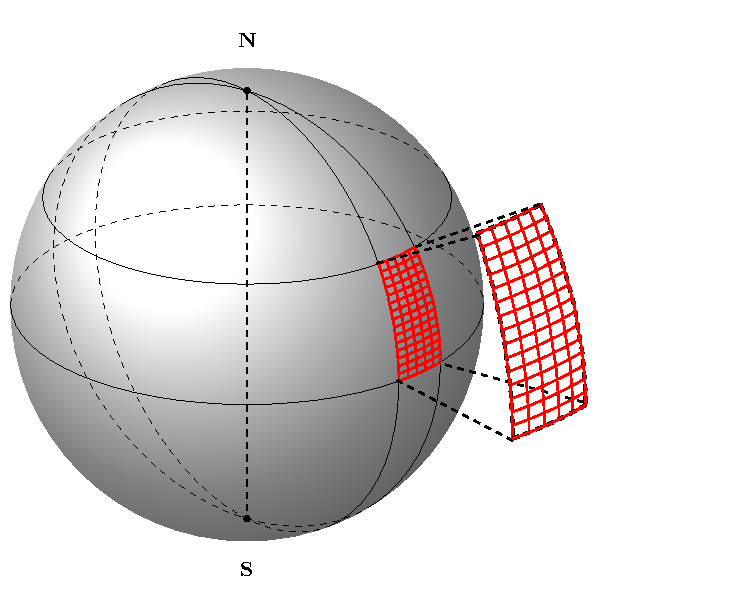
\includegraphics[width=.99\linewidth]{img/sphere-decomp.pdf}
  \caption{Grid-point model decomposition}
  \label{fig:sub1}
\end{subfigure}%
\begin{subfigure}{.5\textwidth}
  \centering
  \includegraphics[width=.99\linewidth]{img/waves.png}
  \caption{Spectral model decomposition}
  \label{fig:sub2}
\end{subfigure}
\caption[Grid-point and spectral domain decomposition]{A simplified example of a grid-point and spectral model projected onto the sphere. This example uses just 3 waves, which implies a truncation of T3. Most spectral models use a resolution in excess of 21 waves (T21). }
\label{fig:test}
\end{figure}
\par
Spectral models represent the spatial variations of atmospheric variables as a finite series of waves at various wavelengths, whereby each wave represents the coefficients of a known function \cite{bourke1988spectral}. They are typically used for global climate modelling rather than regional weather prediction as wave functions and spherical harmonics operate over a spherical domain. Because of this, all waves must be periodic so that they wrap around the sphere with the start and finish point using the same value. This places some restrictions on the type of algorithm that can be used, and can add an additional overhead to compute costs as the model must convert into a spatial representation for analysis \cite{orszag1974fourier}. 
\par
Calculating the equations of motion requires solving many partial derivatives in space. Partial derivatives of waves are calculated by summing the derivatives of each basis function, providing an exact result. In contrast, grid-point models must solve partial derivatives by finite differences, and therefore require a higher resolution to provide a comparable degree of accuracy \cite{bart1998coordinate}. 

\subsubsection{Resolution} 
The spatial resolution of a climate model describes the variation in the total amount of data that is used for a given problem size. The resolution of a grid-point model describes the number of grid cells that the model operates over \cite{goosse2010introduction}. A higher cell resolution implies a greater number of cells contained within a grid. Spectral models vary their resolution using a truncation, which refers to the number of waves used to define atmospheric variables \cite{goosse2010introduction}. In both cases, there is a trade-off between resolution and model runtime whereby higher resolutions generally result in longer runtimes, but more accurate results. 
\par
Climate models have a variable temporal resolution, which refers to the amount of model time that passes in the simulation between calculations. Similarly to spatial resolution, the computational intensity of the simulation is influenced by the granularity of the temporal resolution. Smaller time steps more accurately represent continuous time, but result in longer runtimes.
\par
Both grid-point and spectral models are usually classified as a strong scaling problem, for which the solution time varies with the number of processors for a fixed problem size \cite{colella2007performance}. This implies that the runtime decreases as the number of processor cores increases, however this is not always the case and is dependant on the problem domain.


\subsection{Fast Fourier Transform}
The Isca model uses both grid-point and spectral methods for domain decomposition. A grid-point representation is used for time-stepping, and the physics simulation is applied in the spherical and frequency domains. To convert between these two states, a \gls{fft} is used to compute the \gls{dft} of the grid-point representation, and the \gls{idft} of the spectral representation. Although the cost of doing this transformation can be relatively high, it often results in a net computational saving, and can produce more accurate data at lower resolutions \cite{bader2008climate}. Spectral methods are one of the `seven dwarfs' of HPC popularised by Asanovic \textit{et al.} in 2006, and describe operations applied to data in the frequency domain \cite{asanovic2006landscape} .
\par
The \gls{fft} algorithm is found across many different scientific domains, and as such writing optimised \gls{fft} code is a research topic in and of itself \cite{singleton1967method, cooley1965algorithm, sorensen1987real}. There are multiple highly optimised \gls{fft} libraries available, and there are many different approaches to applying the algorithm, each with their own benefits and drawbacks. This research project uses the \gls{fftw} library, which was developed by Matteo Frigo and Steven G. Johnson at the Massachusetts Institute of Technology, and first released in 1997 \cite{frigo1998fftw}. 

\subsection{The Fastest Fourier Transform in the West}
\gls{fftw} is an implementation of a \gls{dft} that adapts to the hardware on which it is run \cite{frigo2005design}. The library has been written in ANSI C, however it provides interfaces for other programming languages including Fortran. Rather than providing a hand-tuned implementation for all possible hardware configurations, FFTW uses a plan to precompute various sub-arrays based on the shape, size and memory layout of the input data, without requiring the data itself \cite{frigo2005design}. The planning process yields a plan, which is an executable data structure that returns the DFT of the given input data. 
\par
To create a plan optimised for the hardware on which the code is compiled, the planner measures the runtime of many different plan configurations and returns the plan that results in the quickest runtime \cite{frigo2005design}. The planning process is computationally expensive, however it is only performed once, and the resulting plan can then be reused on different input data of the same dimensions. If many FFTs of the same type are repeatedly called in an application, this generally provides a net performance gain \cite{frigo2003fftw}.
\par
Plans are created using FFTW's own compiler called \texttt{genFFT}  \cite{frigo2005design}. Whilst the FFTW library itself is written in ANSI C, \texttt{genFFT} is written in Objective Caml, and is used to produce a number of small hard-coded transforms called codelets. Codelets are well-optimised simple straight line programs, which compute the DFT of a small sequence of data. The speed of FFTW is largely accredited to these codelets, which are successively applied to sections of a larger sequence \cite{frigo2005design}. 
\par
Although not a requirement of using FFTW, the input data should be contiguous in memory so that vector instructions can be utilised. FFTW version 3.3.8 officially supports AVX x86 extensions and version 3.3.1 introduced support for the ARM Neon extensions \cite{frigo2003fftw}. Version 3.3.8 of the library was chosen for this implementation to target the vector extensions on all hardware configurations used in this research project. 


\subsubsection{Cooley-Tukey algorithm}
Despite FFTW using many different FFT algorithms, the most commonly used is the Cooley-Tukey algorithm. This algorithm was popularised in 1965, however variations of the algorithm have been known as early as 1805 \cite{cooley1965algorithm, heideman1985gauss}. Proper implementation of the Cooley-Tukey algorithm results in a time complexity of $O(n\, \textrm{log}\, n)$. The algorithm is based on the assumption that a DFT of size $N = n_{1} \cdot n_{2}$ can be expressed as a two-dimensional DFT of size $n_{1} \times n_{2}$ \cite{frigo2005design}. The algorithm itself can be broken into three steps: 

\begin{enumerate}
	\item Perform $n_{1}$ DFTs of size $n_{2}$;
	\item Multiply by some \textit{twiddle factors}, which are a constant complex coefficient that is multiplied by the input data in order to recursively combine small DFTs \cite{gentleman1966fast};
	\item Perform $n_{2}$ DFTs of size $n_{1}$.
\end{enumerate}

When presented with this information, it becomes clear why the authors of FFTW decided to use a codelet-based design. An optimal solution to performing the FFT using the Cooley-Tukey algorithm allows for a codelet to calculate the DFT on a number of data structures of either size $n_{1}$ or $n_{2}$.

\subsubsection{One-dimensional real-data DFT}
FFTWs real input DFT computes a forward transform $Y$ of a real-type input array $X$ of size $N$, whereby a forward transform refers to a negative sign before the exponent \cite{frigo2005design}. The output of this transform will be a complex-type array of size $N/2$, where the $k^{th}$ output corresponds to the frequency $k/N$. Equation \ref{eq:fftw-forward} shows the forward FFT used by the FFTW library.

\begin{equation}
Y _ { i } = \sum _ { j = 0 } ^ { N - 1 } X _ { j } \cdot e ^ { - 2 \pi i j \sqrt { - 1 } / N }
\label{eq:fftw-forward}
\end{equation}

\subsubsection{One-dimensional complex-data DFT}
FFTWs complex input DFT computes a backward transform $Y$ of a complex-type input array $X$ of size $N/2$ \cite{frigo2005design}. The only difference between the forward and backward transform is the sign of the exponent, which is positive for the backward transform. The output of the backward transform is a real-type array of size $N$. Equation \ref{eq:fftw-backward} shows the backward FFT used by the FFTW library.
\begin{equation}
Y _ { i } = \sum _ { j = 0 } ^ { N - 1 } X _ { j } \cdot e ^ { 2 \pi i j \sqrt { - 1 / N } }
\label{eq:fftw-backward}
\end{equation}


% - - - - - - - - - - - - - - - - - - - - - - - - - - - - - - - - - -
% Chapter - Porting - - - - - - - - - - - - - - - - - - - -
% - - - - - - - - - - - - - - - - - - - - - - - - - - - - - - - - - -
\section{Software architecture}
The Isca codebase is vast, composed of over 290 Fortran90 source files. As it would be impractical to review to entire codebase within the scope of this project, the following section provides a brief introduction to the software architecture of the model.
\subsection{General overview}
Isca is compiled and run using its own Python library, which is used to populate various Bash scripts, Fortran namelists and other miscellaneous files with data entered into multiple dictionaries in a Python script. This was a design decision based on the usability of Python in comparison to the underlying Fortran model, and allows for a lower barrier to entry in terms of technical ability for climate researchers \cite{vallis2018isca}. 
\par
\begin{figure}[H]
\begin{center}
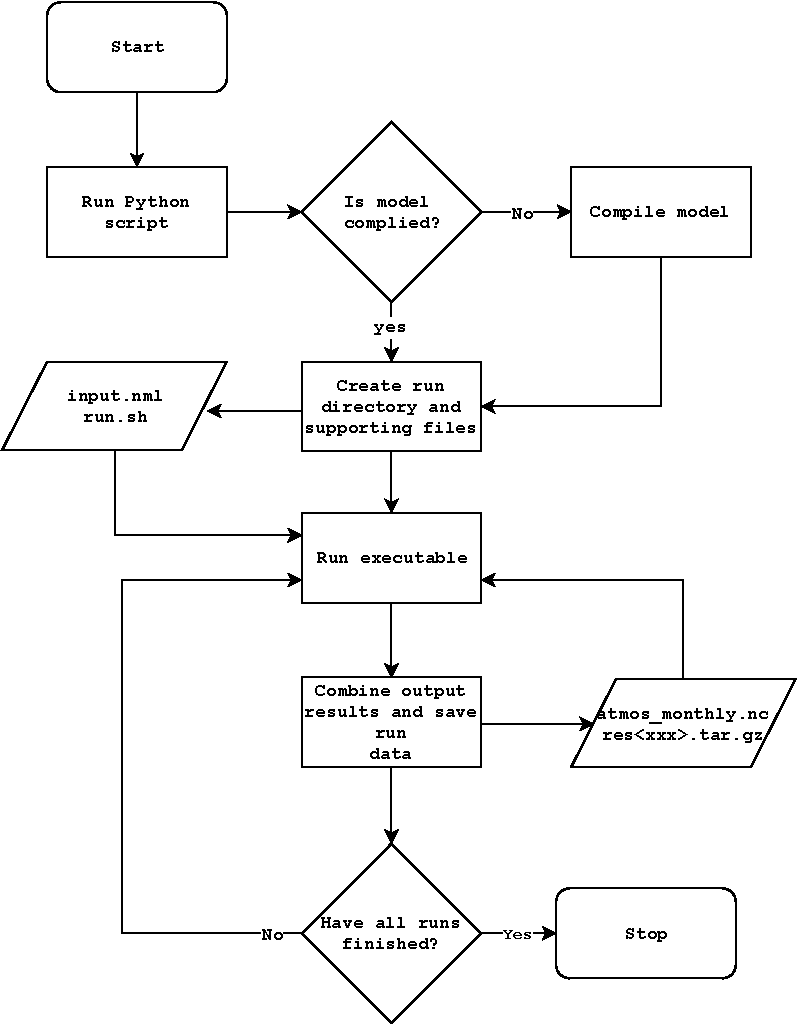
\includegraphics[width=0.75\textwidth]{img/isca_flow.pdf}
\caption{Flowchart illustrating the program flow of Isca, when run using its Python library. The \texttt{run.sh} Bash script is repeatedly used to run the Isca executable.}
\label{fig:flowchart}
\end{center}
\end{figure}
\par
Compiling the model using the Python library produces a single executable that is repeatedly run for a number of epochs defined in a Python script. The length of each epoch is variable, usually lasting for approximately one model month but simplified to 30 model days. When run in parallel the diagnostic output is distributed, which means that each processor writes its own files. Upon completion, the data generated by the previous month's simulation is combined into a single file, and is used as an input to the following month (Figure \ref{fig:flowchart}). The large number of Python and Bash scripts used to create directories, populate and move supporting files means that the executable cannot be run alone.

\par
\par
The executable itself follows an `atmosphere integration loop', whereby the state of the atmosphere is computed for a predefined number of time steps. The modularity of Isca allows for the atmosphere to be simulated using a wide range of different techniques and algorithms at varying degrees of complexity and realism, however the most basic atmosphere integration loop is visualised as pseudocode in Listing \ref{code:atmos-integration}.

\begin{lstlisting}[language=Fortran,label={code:atmos-integration},caption={Pseudocode for the atmospheric integration loop found in Isca.}]
Time_next = Time + Time_step

if(idealized_moist_model) then
   call idealized_moist_phys(...)
else
   call hs_forcing(...)
endif

call spectral_dynamics(Time, ...)

if(dry_model) then
  call compute_pressures_and_heights(x, z, ...)
else
  call compute_pressures_and_heights(x, y, ...)
endif

call spectral_diagnostics(Time_next, ...)

previous = current
current  = future
\end{lstlisting}
\par
The atmosphere integration loop contains many subroutines, however of greatest interest is the \texttt{spectral\_dynamics} subroutine, which comprises around 95\% of the wallclock runtime of any given simulation (Listing \ref{code:atmos-integration}). This subroutine calculates values for various atmospheric variables, which involves  communication between processors and a number of FFTs. 
\par
Isca's spectral model decomposes the horizontal grid into latitude bands, with each band assigned to a processor. When only two processors are used the grid is split into Southern and Northern Hemispheres \cite{isca2019github}. This method of domain decomposition implies that atmospheric variables at the edge cases of each latitudinal band (halo points) must be exchanged with other processors in a process known as a synchronised halo exchange. This allows for parallelism in the Isca model at the cost of an additional overhead incurred by the communication itself. The halo exchange simply interrupts the computational flow of the program and allows for the exchange of the halo points before the simulation can resume (Figure \ref{fig:halo-exchange}).

\begin{figure}[htbp]
\begin{center}
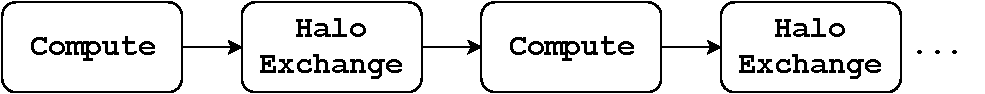
\includegraphics[width=0.7\textwidth]{img/comm_pattern.pdf}
\caption[Simple halo exchange]{Simple communication pattern. Sections of compute are interrupted by calls to a halo exchange.}
\label{fig:halo-exchange}
\end{center}
\end{figure}


\subsection{Dependencies}
\label{sec:dependencies}
\subsubsection{Fortran Libraries}
Isca relies on MPI for interprocess communication and NetCDF for data storage. These technologies are commonly used in high performance computing and offer interfaces for both the ANSI C and Fortran programming languages \cite{mpi2015standard, rew1990netcdf}.

\begin{description}
	\item[MPI] \gls{mpi} is a standardised, portable interface for interprocess communication that allows for direct data transfer between processors without relying on shared memory \cite{mpi2015standard}. The MPI standard has been implemented by numerous companies and organisations but the most commonly used are OpenMPI, MVAPICH, MPICH, and Intel MPI. All MPI implementations provide the same function calls and interfaces, and can therefore be used interchangeably. 
	
	\item[NetCDF] Network Common Data Format (NetCDF) is a platform independent binary file type that is commonly used to store and analyse scientific data \cite{rew1990netcdf}. NetCDF binary files are self-describing, containing all the necessary information to interpret the data they store. This makes NetCDF files highly portable as a file written on one computer can be read by another without context or specialist tools, aside from the NetCDF library itself. If compiled using an MPI library, NetCDF can provide parallel IO. NetCDF itself is dependant on the HDF5 and zlib libraries, which are used for storage and data compression, respectively. When compiling the NetCDF library or any program that uses it, the same compiler must be used to compile HDF5, zlib, NetCDF and the program itself. One of the advantages of NetCDF is that there are many programs available to visualise the data they store (Figure \ref{fig:netcdf}). 
\end{description}

\begin{figure}[htbp]
\begin{center}
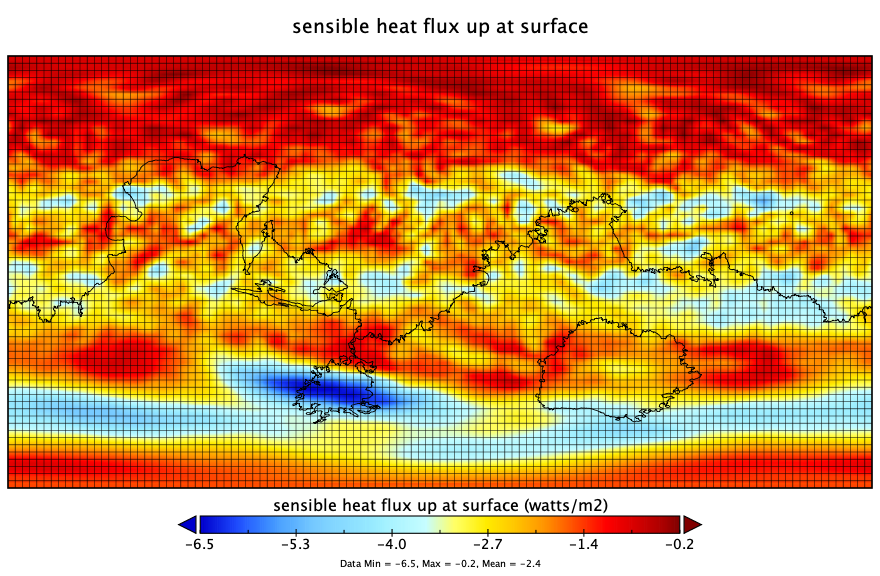
\includegraphics[width=\textwidth]{img/flux_t_in_atmos_daily.png}
\caption[Visual output from the Isca model]{Visualisation of an output of from the Isca model running a Grey-Mars radiation model. The image shows the heat transfer to the Martian surface after 690 days. This visualisation was generated using the Panoply NetCDF data viewer tool \cite{schmunk2015panoply}.}
\label{fig:netcdf}
\end{center}
\end{figure}

\subsubsection{Python libraries}
For simplicity, Isca uses a Python interface to create and run different model configurations. To do this, it uses a number of popular Python libraries that are commonly available on many different platforms.

\begin{description}
	\item[Numpy] A mathematics library for Python that allows for the manipulation of N-dimensional arrays \cite{van2011numpy}.
	
	\item[sh] A full-featured subprocess replacement for Python that allows for Bash commands to be issued from Python code \cite{moffat2017sh}. 
	
	\item[Jinja2] A templating language for Python that is typically used in web design. It has been used in Isca to populate a number of Bash script templates with data defined in a series of Python dictionaries \cite{ronacher2008jinja2}. 
	
	\item[f90nml] A Python module and command line tool for reading, writing and modifying Fortran namelist files \cite{wardf90nml}. 
	
\end{description}








\chapter{HPC hardware and parallel processing}
There are many different techniques and processor designs that allow for a program to be run in parallel. This chapter presents a brief but thorough overview of some that have been used throughout this research project. 

\section{Parallel processing}
To allow for programs to be run in parallel, there are numerous different techniques that can be used. In order to improve the performance of a parallel code, understanding of these techniques are essential.

\subsection{Flynn's Taxonomy}
Flynn's taxonomy is a classification of parallel computing architectures first proposed by Michael J Flynn in 1966 \cite{flynn1972some}. It defines four unambiguous terms to describe the relationship between data and the technique by which it is processed. The entirety of Flynn's taxonomy is visualised in Figure \ref{fig:Flynn's}, and the following bullet list details the architectures it describes.

\begin{description}
	\item[Single Instruction Single Data (SISD)] refers to the most basic type of processing whereby a single instruction is applied to a single data item stored in memory. Code that uses this processing type is often referred to as scalar or serial. 
	
	\item[Single Instruction Multiple Data (SIMD)] allows for a single instruction to be applied to multiple data items stored in a contiguous piece of memory. To gain the largest performance benefit from SIMD operations, the multiple data items must be read using a single instruction, and then the same operation must be applied to all items. SIMD processing is often referred to as vectorisation, as the data is processed as a one-dimensional vector. 
	
	\item[Multiple Instruction Single Data (MISD)] is a rarely used processing technique that applies different operations on identical data. Rather than improving the performance of a program, it is often used for mission critical computations where there is no room for error. 
	
	\item[Multiple Instruction Multiple Data (MIMD)] is currently the most commonly used parallel processing technique. It describes a machine that contains many asynchronous processors that function independently, and as such, most modern processors can be categorised as MIMD.
\end{description}
\par
\begin{figure}[htbp]
\begin{center}
\includegraphics[width=0.8\textwidth]{img/Flynns.pdf}
\caption[Flynn's taxonomy]{Flynn's taxonomy. Instructions are applied to data by various processing elements (PE) in different ways. }
\label{fig:Flynn's}
\end{center}
\end{figure}
\par
Like most scientific codes, Isca uses the SIMD and MIMD approaches to parallelism. As discussed in Section \ref{sec:dependencies}, the model uses the MPI library to split the domain into latitude bands. Modern processors also have wider registers in order to apply a data-level parallelism technique whereby multiple data items are processed by a single instruction. 

\subsection{Instruction-level parallelism (SIMD)}
From the 1970s to the early 1990s, high performance machines relied heavily on instruction level vector operations to compute in parallel \cite{6877473}. These machines used vector processors, and performed operations on one-dimensional arrays of data, rather than single data items using a SIMD processor architecture \cite{conte2000long}. Many scientific codes from this time were written with this architecture in mind and it is likely that it influenced the design and implementation of the FMS. 
\par
Instruction-level parallelism using SIMD is becoming popular once again through the introduction of Intel's \gls{avx}. Intel introduced AVX in 2011's Sandy Bridge architecture, AVX-2 in 2013's Haswell architecture and AVX-512 in 2016's Skylake architecture \cite{chris2011avx, intel2019avx}. AVX increased the width of some vector registers to 256 bits, allowing for SIMD operations on four 64-bit elements per clock cycle. In comparison, the AVX-512 instruction set increased vector register width to 512 bits, allowing for SIMD operations on eight 64-bit elements per clock cycle, double that of AVX and AVX-2 \cite{chris2011avx,xeon2680v4}.
\par
Although AVX-512 has a higher throughput of operations per clock cycle, using wider vector registers results in greater power consumption, which in turn causes the processor to generate more heat. In order to maintain a suitable temperature, Intel processors perform dynamic frequency scaling in order to decrease the clock speed for the duration of the loop using the AVX-512 registers, often resulting in no overall performance gain over AVX-2 \cite{gottschlag2018mechanism}.

\section{HPC clusters}
Throughout the course of this research project, Isca has been ported to and run on four different high-performance supercomputers. This section discusses these machines, and the features of their respective processor architectures. A full breakdown of the most important hardware features can be found in Table \ref{tbl:hardware}. \gls{bcp3}, \gls{bcp4} and \gls{bp} are all based on the well-established line of x86-64 Intel Xeon processors and Isambard is based on the ARM-v8 Cavium ThunderX2 processor.
\begin{table*}[!ht]
\centering
\caption[Hardware specifications of the target HPC systems]{Hardware specifications of the target HPC systems. }
\begin{tabular}{@{\extracolsep{4pt}}ccccc}
\toprule 
\multirow{2}{*}{\textbf{Attribute}} & \multicolumn{3}{c}{\textbf{Intel Xeon (x86-64)}} & \multicolumn{1}{c}{\textbf{ARMv8}}\\

				\cmidrule(lr){2-4} \cmidrule(lr){5-5}

 				& {\textbf{BCP3}} 	& {\textbf{BCP4}} 		& {\textbf{BP}} 		& {\textbf{Isambard}} \\
\midrule
%Machine		   	& blank		    	&blank				&					& Cray XC50 	\\
Processor	   		& E5-2670 v1 		& E5-2680 v4			& Gold 5120			& ThunderX2	\\
Codename            	& Sandy Bridge	        & Broadwell         		& Skylake       		   	& ThunderX2   	\\
Instruction set		& AVX			& AVX-2				& AVX-512			& NEON		\\
Clock Speed	   	& 2.6 GHz		    	& 2.4 GHz				& 2.2 GHz				&  2.1 GHz 	\\
Cores / Node		& $2\times8$		& $2\times14$			& $2 \times 14$			& $2\times32$	\\
Memory / Node		& 64 GB			& 128 GB				& 256 GB					& 256 GB		\\
Compute Cores		& 3,568		    	&14,700				& -					& 10,752 		\\
Interconnect		&  QDR InfiniBand	& Omnipath			& Ethernet			& Cray Aries	\\
\bottomrule
\end{tabular}
\label{tbl:hardware}
\end{table*}

\subsection{BlueCrystal phase 3}
\gls{bcp3} is primarily intended for smaller jobs that run on a single node, and it is the oldest cluster still in use at the University of Bristol. A single node of \gls{bcp3} contains two, eight-core Sandy Bridge Xeon E5-2670 v1 processors, which were the first line of the Intel processors to use \gls{avx}, increasing the width of vector registers to 256-bits. 

%%and a node of \gls{bcp4} contains two, fourteen-core Broadwell Xeon E5-2680 v4 processors. Although the Broadwell processor has a lower base clock rate than the Sandy Bridge processor, it incorporates more processing cores, and also has a larger memory-bandwidth. Additionally, it has wider registers due to the inclusion of the AVX-2 instruction set.

\subsection{BlueCrystal phase 4}
\gls{bcp4} has been the University of Bristols main workhorse cluster since 2017. It was designed and configured by OCF in collaboration with Lenovo and is primarily intended for large parallel jobs across multiple nodes. \gls{bcp4} now has an established userbase, however the machine is almost at maximum capacity and some longer jobs can spend over a week in the queue before they run.
\par
A compute node of BCP4 contains two fourteen-core Broadwell Xeon E5-2680 v4 processors. They use the AVX-2 instruction set architecture and were introduced by Intel in 2016, 

\subsection{BluePebble}
\gls{bp} is a new Intel-based cluster, managed by the \gls{acrc} at the University of Bristol. It was created in order to ease congestion on \gls{bcp4} by moving some of its heaviest users to their own cluster with dedicated resources. Some members of the meteorological research group at the University of Bristol can be classified as heavy users of \gls{bcp4}, and have recently purchased a £10,000 dedicated node of BluePebble to conduct their research using Isca. 
\par
\gls{bp} contains two different types of compute node, both using Intel's Skylake architecture. The first contains two twelve-core Xeon Gold 6126 processors and the second contains two fourteen-core Xeon Gold 5120 processors. Both processors make use of AVX-512 instruction set. 


\subsection{Isambard}
The GW4 Alliance, which consists of the Universities of Bath, Bristol, Cardiff and Exeter, together with the UK Met Office and Cray Inc have worked together to deliver the Isambard supercomputer, which is the result of a £3m award by the \gls{epsrc} \cite{arm2018white}. Isambard provides multiple advanced architectures, however the focus of this research project is the Arm-based Cavium ThunderX2 processor, which forms the basis of the machine. Each of Isambard's 168 compute nodes contain 64 ARMv8 cores in a dual-socket configuration \cite{thunderprocessor2018brief}. 

%An important feature of the ThunderX2 is that it has eight memory controllers per socket, which results in a peak theoretical memory-bandwidth in excess of 250 GB/s \cite{mcintosh2018performance}. 


\subsubsection{Cavium ThunderX2 Server Microprocessors}
Arm primarily designs processors for mobile devices and has only recently produced hardware optimised for HPC systems \cite{mcintosh2018performance}. Due to the heat generated by high clock rates, modern chip designers are now limited by power consumption. Because of this constraint, the current trend in supercomputer design is to use large shared-memory nodes, that use higher core cores and decreased clock rates \cite{kindratenko2011trends}. 
\par
Arm processors have inherently low power consumption as they were originally designed for mobile devices. Because of this, the European Mont-Blanc project began to investigate the potential of the Arm architecture for \gls{hpc} in 2011 \cite{Rajovic:2016:MPA:3014904.3014955}. This project proved to be successful, however the study uncovered some problems with the architecture that have since been addressed during the development of the ThunderX2. ThunderX is a line of 64-bit many-core server microprocessors developed by Cavium as a result of over 8 years of work by the Mont-Blanc project and other contributors. The ThunderX2 was first released in early 2018 as the successor to the ThunderX, and is the first generation of Arm-based server microprocessors intended for high performance computing. Initial studies have found that the ThunderX2 presents as a real alternative to current offerings by vendors of desktop hardware, finding that the processor delivers competitive levels of performance to Intel's line of Xeon processors \cite{calore2018advanced, mcintosh2018performance}. 
\par
\begin{figure}[htbp]
\begin{center}
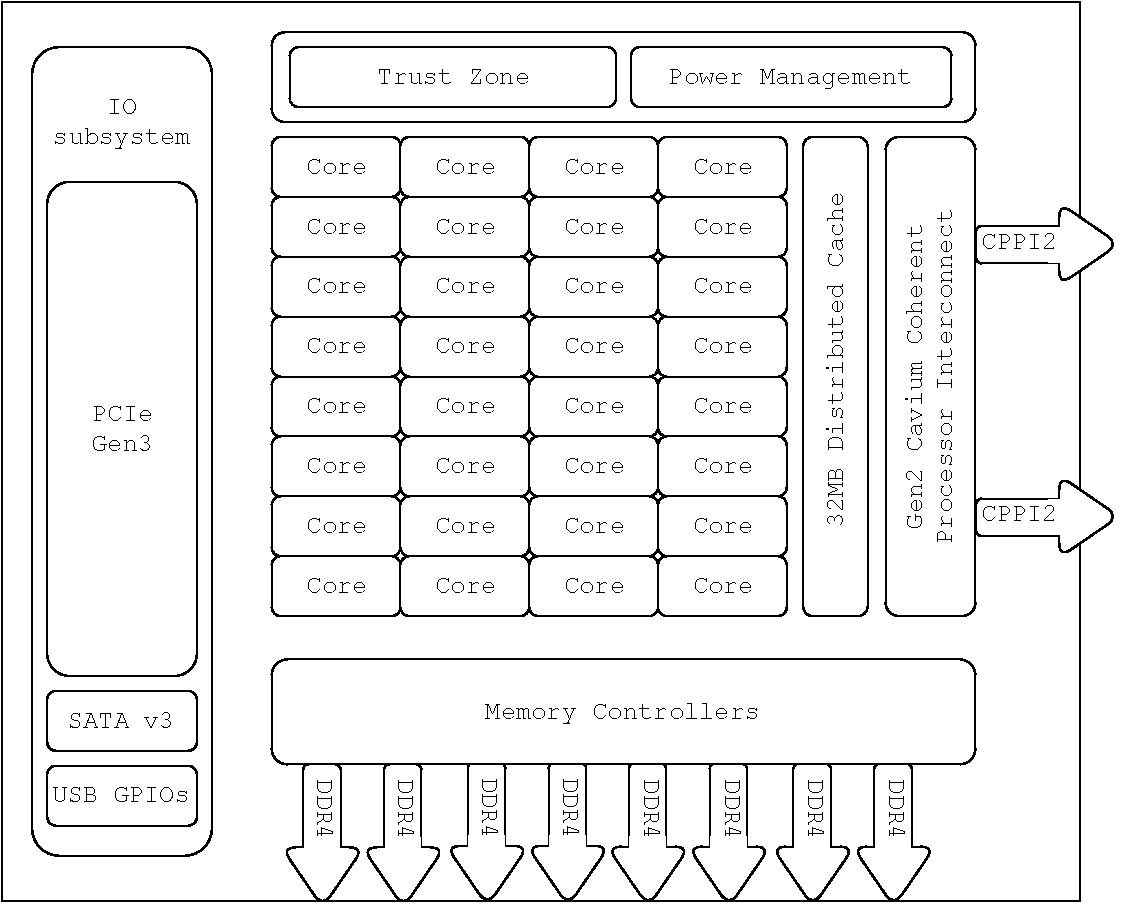
\includegraphics[width=1\textwidth]{img/thunderx2.pdf}
\caption[Block diagram of the Cavium ThunderX2 server microprocessor]{Block diagram of the Cavium ThunderX2 server microprocessor. Diagram redrawn from \cite{thunderprocessor2018brief}}
\label{fig:thunderx2}
\end{center}
\end{figure}
\par
The ThunderX2 uses the ARMv8.1 instruction set, which allows for the use of 128-bit NEON SIMD vector registers. Perhaps the most interesting feature of the ThunderX2 as noted by McIntosh-Smith \textit{et al.} is its eight memory controllers per socket, which have been demonstrated to produce a memory bandwidth in excess of 250GB/s \cite{mcintosh2018performance}. The layout of the processor is shown in Figure \ref{fig:thunderx2}.

\subsubsection{A64FX}
To meet the compute requirements of future HPC workloads, Fujitsu has recently announced the next generation of Arm chips in their A64FX processor. The A64FX improves upon the NEON instruction set found in the ThunderX2 by introducing \gls{sve}, which allow for a flexible vector register length between 128 and 512 bits so that vector length can reflect the compute requirements of different use cases \cite{stephens2017arm, rico2017arm}. These processors have not yet been released, however this thesis provides an estimate of their performance based on the performance of the ThunderX2.


\chapter{Benchmarking and performance analysis}
This chapter is an introduction to benchmarking both hardware and software, and describes some of the techniques and metrics used to benchmark the Isca code. 
\section{Cluster benchmarks}
\label{sec:cluster-bench}
The STREAM TRIAD and \gls{hpl} benchmarks have been used to measure the peak memory bandwidth and floating point performance of each node configuration used in this study, respectively. This has been done to provide a relative performance overview of each processor architecture and to highlight the differences between them. 

\subsection{STREAM TRIAD}
The speed of processors has increased exponentially over the past twenty years as described by Moore's law, which states that the number of transistors in a dense integrated circuit doubles approximately every two years  \cite{moore1965cramming}. In comparison, the speed of memory has only marginally improved as manufacturers have historically prioritised memory capacity over speed \cite{mccalpin1995memory,patterson1997case}. The result of this is that many scientific codes are no longer bound by compute, but by the rate at which data can be read from or stored to memory by the processor. The STREAM memory-bandwidth benchmark was introduced by John McCalpin in 1995 to address the limitations of the benchmarks of the time, and to measure processor performance by its peak memory bandwidth consumption rather than the rate of \gls{flops}.
\begin{figure}[htbp]
\begin{center}
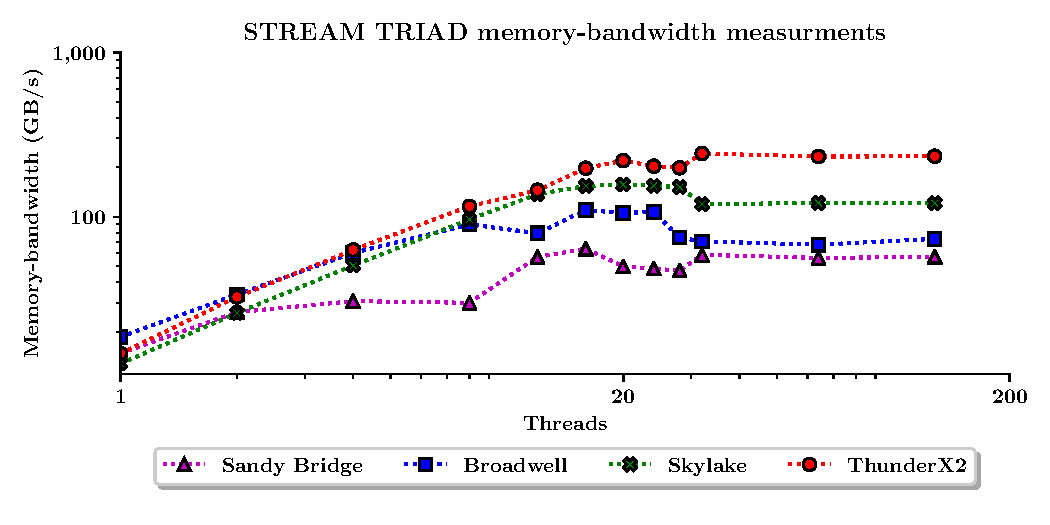
\includegraphics[width=0.7\textwidth]{img/stream-triad.pdf}
\caption[STREAM TRIAD benchmark]{STREAM TRIAD results for all processor architectures that have been used as part of this research project. }
\label{fig:bandwidth}
\end{center}
\end{figure}
\par 
As core counts and memory channels continue to grow, it becomes increasingly difficult to measure the memory bandwidth of modern processors, and results can greatly vary depending on the system configuration used to compile and run the benchmark. The results shown in Figure \ref{fig:bandwidth} were collected using the original STREAM benchmark code \cite{stream2019github}. The code was compiled using the Intel compiler with the same flags and environment variables on each cluster with the exception of the ThunderX2 processor, which used the GNU compiler. 
\par
The ThunderX2 processor has eight memory controllers per socket, and presents a peak STREAM TRIAD result in excess of 240 GB/s for a dual-socket configuration. In comparison, the Skylake processor provides a result of just 157 GB/s. This observation alone is a testament to the class leading memory bandwidth of the ThunderX2.

\subsection{High Performance Linpack}
The theoretical peak performance of a compute node can be calculated (Equation \ref{equ:perf}). $c$ denotes the processor speed in GHz, $p$ denotes the number of processor cores, $i$ denotes the number of instructions per clock cycle, and $o$ denotes the number of processors per node. 

\begin{equation}
GFLOPS = c \cdot p \cdot i \cdot o 
\label{equ:perf}
\end{equation}
\par
Generally, the theoretical peak performance of a machine is unattainable. The \gls{hpl} benchmark aims to measure the attainable percentage of peak processor performance by solving a dense system of $n\times n$ linear equations \cite{dongarra2008linpack}. Figure \ref{fig:hpl} shows the actual performance measured using the \gls{hpl} benchmark compared to the peak theoretical machine performance calculated using Equation \ref{equ:perf}. 
\par
\begin{figure}[htbp]
\begin{center}
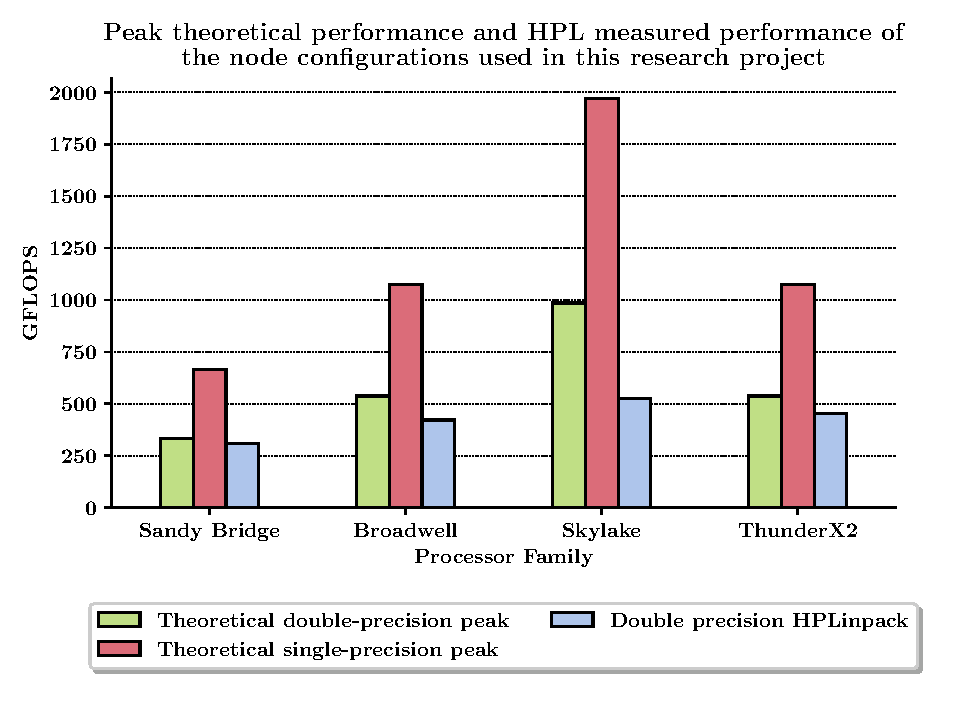
\includegraphics[width=0.85\textwidth]{img/hpl.pdf}
\caption[High performance Linpack benchmark]{Comparison of the theoretical peak machine performance against the performance measured by HPLinpack. }
\label{fig:hpl}
\end{center}
\end{figure}
\par
The performance measured using the HPLinpack benchmark is less than the theoretical performance in all cases. The large theoretical peak performance of the Skylake processor is attributed to its wide 512-bit vector registers, which can process 16 double-precision floating point numbers with a single instruction. The signifcantly smaller actual performance measurement is because the processor can only use AVX-512 at a reduced clock rate, and therefore the compilers performance model rarely opts to use these registers. 

\section{Application benchmarking}
\label{sec:app-benchmarking}
Floating point performance and memory bandwidth are usually measured using idealised techniques like the STREAM and HPLinpack benchmarks, and may not provide the best metrics for a complex code like Isca. Although the model is computationally demanding there is also a large overhead cost incurred by communication. This includes tasks such as reading and writing files, the movement of data into contiguous memory and the transmission of data between processors. For this reason, the model can only be expected to achieve a fraction of the theoretical peak memory bandwidth and floating point performance reported in the previous section. Therefore, the following performance metrics have been defined, and are used throughout this study.
\subsection{Performance metrics}

\subsubsection{Wallclock runtime} 
Wallclock runtime refers to the total amount of real time that has passed from the start of the program to the end. In this study, wallclock runtime has been reported in seconds. Used alone, this metric does not provide a basis for comparison between other configurations and therefore three other metrics have also been used.
	
\subsubsection{Speedup} 
Speedup is a measure of relative performance between two solutions for the same problem. For the metric reported in this study, this is the number of times faster the code ran than some other given benchmark, typically the serial runtime. The speedup $S$ of a code can be calculated given two runtimes $R_1$ and $R_2$ using the formula in Equation \ref{equ:speedup}, whereby $R_1$ is $S\times$ faster than $R_2$ \cite{kumar1994analyzing}.
\begin{equation}
S = \frac{R_1}{R_2} 
\label{equ:speedup}
\end{equation}
	
\subsubsection{Cost per gridpoint}
Other studies that have benchmarked parallel climate codes have used the \gls{ccpgpt} as a primary performance metric as it takes into account the cost of interprocess communication \cite{schmidt2007benchmark}. When run on a single core, 100\% of the program runtime is spent on computation. As the number of processor cores increases, a larger portion of the runtime is spent on communication and therefore the cpu time taken to compute a single grid-point increases. The amount of consumed compute resources $T_p$ for a given simulation can be calculated given the wallclock runtime $t$ and the number of processors used $p$, as shown in Equation \ref{equ:comp-cost}.
\par
\begin{equation}
T_p = t \cdot p
\label{equ:comp-cost}
\end{equation}
To provide a meaningful comparison between core counts, the \gls{ccpgpt} must be calculated. Given the number of timesteps $N_t$ and number of grid points $N_g$, we can calculate the total simulation \gls{ccpgpt}, $C_{tg}$ as shown in Equation \ref{equ:cost}. 

\begin{equation}
C_{tg} = \frac{T_p}{N_t \cdot N_g}
\label{equ:cost}
\end{equation}
Although increasing MIMD parallelism by introducing additional processor cores decreases the overall runtime, a greater portion of the runtime is spend idle waiting for data to be sent between processors. The $C_{tg}$ metric doesn't discriminate based on wallclock runtime, and provides a solid basis for comparison between model resolutions and number of processor cores. 

\subsubsection{Operational intensity}
The operational intensity $I$ of a code or compute kernel is defined as the ratio of work $W$ to the memory traffic $Q$ \cite{williams2009roofline}. It is a commonly used metric to assist in the identification of performance bottlenecks of high-performance codes, especially when used together with a roofline model \cite{williams2009roofline}. Operational intensity is formally defined in Equation \ref{equ:oi}.

\begin{equation}
\label{equ:oi}
I = \frac{W}{Q}
\end{equation}
\par
For the analysis performed in this research project, $W$ denotes the number of \gls{flops}, and $Q$ denotes the total amount of memory transferred in Bytes. This results in operational intensity measured in FLOPS/Byte. 

\subsubsection{Summary}
To ensure simplicity, the wallclock runtime is the primary performance metric used throughout this paper. However, it is important to consider other metrics as they can uncover important features of the code that are overlooked by runtime alone. Values for all four metrics defined in this section have been calculated using the data collected as part of this research project. 




% - - - - - - - - - - - - - - - - - - - - - - - - - - - - - - - - - -
% Chapter - Porting - - - - - - - - - - - - - - - - - - - -
% - - - - - - - - - - - - - - - - - - - - - - - - - - - - - - - - - -
\let\textcircled=\pgftextcircled
\chapter{Porting}
\label{chap:baselineexp}
In the context of software development, porting refers to the process of modifying an existing codebase in order for it to run on a different system than it was originally written for. This chapter gives an overview of some of the tools and techniques used when porting Isca, and presents some of the challenges encountered in doing so. Many small changes have been made to the codebase to enable the model to compile and run using a selection of commonly-used compilers, some of which can be found in appendix \ref{apdx:porting}. 

\section{Compilers and MPI libraries}
To allow for the best comparison between processors, Isca was compiled using a number of different compilers and MPI libraries. Table \ref{tbl:compilers} shows the different configurations used to compile Isca on each of the clusters used in this study. 

\begin{table}[htp]
\caption{Compilers and MPI libraries used for benchmarking}
\begin{center}
\begin{tabular}{c c c c c}
 \toprule

\textbf{Cluster} 			&	\textbf{Processor Family}		&	\textbf{Fortran Compiler}		&	\textbf{MPI library}	 \\
\midrule
\multirow{2}{*}{BCP3} 	&	\multirow{2}{*}{Sandy Bridge}	&	GNU 7.1.0 			&	OpenMPI	 \\
					& 							& 	Intel 13.0.1			&	OpenMPI			\\
\midrule	
\multirow{2}{*}{BCP4}	&	\multirow{2}{*}{Broadwell}		&	GNU 7.2.0			&	OpenMPI			\\
	&											&	Intel 18.0.3			&	Intel MPI			\\
\midrule	
BP					&	Skylake					&	Intel 19.0.3 			&	Intel MPI			\\
\midrule			
\multirow{2}{*}{Isambard}	&	\multirow{2}{*}{ThunderX2}	&	CCE 8.7.9				&	Cray MPI			\\
					&							&	GNU 8.2.0			&	Cray MPI			\\
%					&							&	Arm $x.y$				&	Cray MPI			\\
\bottomrule \\
\end{tabular}	
\end{center}
\label{tbl:compilers}
\end{table}%
\par
Isca uses a Perl script called \gls{mkmf} to construct makefiles for different model configurations. Before compilation, Isca runs a series of `template scripts' to export environment variables and to load relevant module files to be used by \gls{mkmf}. In order to compile on a new system, a new template script must be written to setup the compilation environment for the machine in question. Although Isca provides some example scripts to do this on existing systems, a new script had to be written for each compiler and processor pair in this study. Two examples of such scripts can be found in Appendix \ref{apdx:compile-env}.  

\subsection{GNU Compiler Collection}
The \gls{gcc} is a selection of compilers for various programming languages and is produced and maintained by the GNU project. \gls{gcc} is available on many different computer architectures, providing the same interfaces and compile flags options on each. This makes it a convenient compiler for porting code, as similar configurations can be used on different machines. The Isca codebase already has an existing \gls{gcc} template script, however it required some minor changes to allow for compilation on each system. This involved selecting the correct module files to be loaded when the script was run, and exporting relevant compiler and linking flags.

\subsection{Intel Compiler Collection}
The \gls{icc} provides numerous premium compilers specifically for Intel-based machines, and is bundled as part of Intel Parallel Studio XE. As Intel develops its compilers alongside its hardware, \gls{icc} generally produces well-optimised instructions, however they are not portable and are limited to Intel processors only. Contained within \gls{icc} is the Intel MPI library, which is focussed on making parallel applications perform better on Intel-based clusters.
\par
The existing Intel template script provided by Isca required few modification to compile the model on each system, however the locations of some libraries needed to be specified. Additionally, the NetCDF library needed to be recompiled using the latest version of the Intel compiler in order to work. 


\subsection{Cray Compiling Environment}
The \gls{cce} is a Fortran 90 compiler developed by Cray Inc. This compiler is relatively new in comparison to the Intel and GNU compilers, and as such is strict to the Fortran standard. This caused many issues when porting the code using this compiler, and flagged up a number of issues with the Isca codebase. The process of porting for \gls{cce} turned into a stringent debugging exercise that has inevitably improved the reproducibility of the code on different platforms. The following subsections describe some of the code changes required to compile and run Isca using the CCE compiler.

\subsubsection{Implicit type conversion}
To provide interprocess communication, Isca uses a `\textit{Massively-parallel} ' module, codenamed MPP. It is a set of simple calls to provide a uniform interface to a collection of commonly used message-passing routines for climate modelling, implemented in different libraries \cite{balaji2002fms}. This module defines many subroutines that depend on the definition of the \texttt{MPP\_DEFAULT\_VALUE\_} macro, which is defined using preprocessor directives at compile time. The \texttt{MPP\_DEFAULT\_VALUE\_} can be assigned as either real, integer or logical. As an extension for backwards compatibility with other compilers, the GNU and Intel compilers allow for the implicit conversion of logicals to numericals and vice versa. When converting from a logical to an integer, the numeric value of \texttt{.false.} is 0, and that of \texttt{.true.} is 1. When converting from integer to logical, the value 0 is interpreted as \texttt{.false.} and any non-zero value is interpreted as \texttt{.true.}. This does not conform to the Fortran 90 standard, which disallows implicit conversion between numeric variables and logicals \cite{fortran1991standard,gnu2019conversion}. This error was found throughout the codebase and changes were made to resolve this issue by creating a new macro \texttt{MPP\_DEFAULT\_TYPE\_}, which is used to define the type of variables assigned using the \texttt{MPP\_DEFAULT\_VALUE\_} macro.

\subsubsection{Namelist read errors}
Isca uses Fortran namelist files to read large numbers of parameters into existing variables and data structures at runtime. Using \gls{cce}, many of the namelist files were being read incorrectly as Isca did not open and close files between separate reads, which caused the code to hang during execution. Additionally, the Cray compiler requires that the representation of the value in the namelist file reflects the type of variable that it will be used for. This means that an integer value must be stored in the namelist as \texttt{variable = 1}, and not \texttt{variable = 1.0}.

\subsubsection{Ambiguous arithmetic}
The Cray compiler required brackets around some arithmetic where it could be considered ambiguous. This was only found in a few places in the codebase, and was trivial to fix. 

\subsection{Discussion}
As the Fortran standard has evolved over the past twenty years, many features that were once commonplace are no longer deemed to fit the language standard, and are not supported by newer compilers. Some of the more popular compilers like \gls{gcc} and \gls{icc} have been updated to allow for backwards compatibility with legacy code, however this is not the case for the \gls{cce} compiler, which strictly follows the Fortran standard.
\par
Both \gls{icc} and \gls{gcc} overlook many negligent programming practices. However to remain portable, codes should be written to the standards of the programming language. Many legacy codes suffer from this issue whereby outdated code remains unchanged throughout many years of use, and part of this research project was to update Isca to improve its portability.


\section{Cluster feedback}
\subsection{Stack size}
Prior to this project, the default stack size on BP was 8 KB. However, as Isca uses a large amount of memory this caused a stack overflow error when running the model at resolutions greater than T42. Due to some configuration restraints on the cluster, the PBS scheduler does not allow for the stack size to be increased using \texttt{ulimit -s unlimited}, as used in Isca's run script. To resolve this issue the default stack size was increased to 64 MB by the system administrator.
\par
As a temporary work around before this issue was resolved, and before interactive jobs were available on the cluster, a regular job can be submitted to the queue that sleeps for an hour in the submission script. The details of the job can be found using the  \texttt{qstat -f <jobid>} PBS command, which can then be used to SSH to the node running the sleeping job. As PBS has not been used to access to the node, the stack size can be increased using the command \texttt{ulimit -s unlimited}, and the code will then run as if in an interactive job. Most of the single-node runtimes for BluePebble were collected using this technique as modifying the cluster configuration was not immediately possible. 

\subsection{Strict processor enforcement}
Isca's Python library is multithreaded, creating additional threads of execution when running experiments. This caused some issues when the model was run on BluePebble as its job scheduler was configured to strictly enforce the CPU limitations defined in the job submission script. After running for an arbitrary amount of time the job would fail as additional Python threads were created, causing the CPU to try to burst past the scheduler limit. This issue took many weeks to fix and required working alongside the BluePebble system administrator. 



\section{Libraries and dependencies}
Although many of the libraries required by Isca were already available as module files, in some cases they were not. This meant that they needed to be built in the \texttt{\$HOME} directory to allow for the model to be compiled. These builds were then used to create module files by the system administrators of the relevant cluster. Throughout the course of the project, the NetCDF, Git, FFTW, Anaconda Python, zlib and HDF5 software packages were installed multiple times using different compilers. 

\section{Development tools}
All code developments were made remotely over SSH and all work was done on the filesystem of each supercomputer. Microsoft Visual Studio Code has a Remote-SSH plugin that allows for files to be edited as if they were on a local machine. This plugin is still in its beta phase of development, and can therefore be unreliable. When it failed, work continued using both the emacs and vim text editors depending on the tools available on the cluster. To allow for code changes to be synchronised across machines, a new fork of the Isca Git repository was created. Each cluster had their own development branch as well as a main development branch for merging changes between them. 



\section{Verification of results}
When porting a codebase it is important to test that the changes made to the code are backwards compatible. This means that all changes must be non-intrusive and configurations must default to the original behaviour. In the case of Isca, all code changes that have been made to run the model on a different cluster have been tested on the BCP4 supercomputer to ensure that they produce the same outputs.

\subsection{Units of last place}
To ensure that the model produces the same results on each system, the model outputs have been checked using the \gls{ulp} numerical analysis technique, which can be used to measure the spacing between floating point numbers. As the whole real line cannot be represented in memory, there is a minimum difference between two numbers occupying the full space offered by floating point numbers \cite{goldberg1991every}. NetCDF files aim to record data in a continuous fashion, which is an impossible task for the discrete numbers used in computational simulations like Isca \cite{rew1990netcdf}.
\par
The outputs of a simulation run by Isca can be verified by comparing the ULP of each parameter in the resulting NetCDF file. As the model is chaotic, even small changes to model parameters can produce vastly different results. However, as the model is not stochastic, the same simulation configuration ran on two separate machines should produce identical results, assuming that the machines store variables to the same degree of precision. 

\subsubsection{Rounding errors}
Rounding errors are a commonly occurring quantisation problem in scientific codes \cite{goldberg1991every}. Although double-precision floating point variables can store numbers to a high degree of precision, they can only store a finite number of digits. Rounding errors are a result of performing arithmetic on continuous numbers in a discrete representation. The IEEE Standard for Floating-Point Arithmetic (IEEE 754) states that all floating point arithmetic must be correctly rounded to within 0.5 ULP of the true mathematical result, therefore any differences greater that 1 ULP suggest inconsistencies in the code \cite{goldberg1991every,ieee1985ieee}. 

\subsection{Program verifcation}
A C++ program was written by Gethin Williams in 2009, and modified for this research project to measure the difference in ULP between NetCDF files obtained on different machines \cite{puma2018}. The program allows for a tolerance to be given to accommodate any rounding errors that may have accumulated throughout the course of the simulation. Due to the differences in compiler and processor architecture a tolerance of 2 ULP was deemed acceptable. All changes to the Isca codebase were verified using this metric.






\part{Benchmarking, performance analysis and optimisation}
% - - - - - - - - - - - - - - - - - - - - - - - - - - - - - - - - - -
% Chapter - Benchmarking and Scaling study - - - 
% - - - - - - - - - - - - - - - - - - - - - - - - - - - - - - - - - -
\chapter{Experimental Methodology}
This chapter outlines the experimental methodology used for benchmarking and analysing the performance of Isca. The collective aim of the following experiments was to characterise the code, to identify potential optimisations and to provide a comparison of the processors themselves.

\begin{description}

	\item[Experiment A: Scaling study] The wallclock runtime taken to complete a simulation for various spatial resolutions and core counts was measured.
	
	\item[Experiment B: Compiler comparison] The per-node performance of the model was compared for two different compilers on each processor, excluding Skylake.
	
	\item[Experiment C: Vectorisation analysis] The per-node performance of the model was measured with SIMD instructions enabled and disabled, to determine the importance of instruction-level parallelism. 
	
	\item[Experiment D: Communication analysis] The interprocess communication times were measured. 
	
	\item[Experiment E: Runtime variation] The wallclock runtime was measured for each epcoh that comprises a full simulation.
	
	\item[Experiment F: Roofline model analysis] A roofline model has been plotted using the operational intensity and double-precision floating point performance of the Isca code, and two compute kernels within it. 
\end{description}
\par
In order to collect reliable data a full node was used for each experiment. Even when run in serial, the model used the resources of an entire node so that the performance would not be affected by shared resource usage by other programs running on the cluster. To account for variations in runtime caused by factors outside the control of the experiment, all runtimes reported in this chapter are the mean value of three repeat measurements, unless stated otherwise. The results presented in the following section are the consequence of over 2,000 hours of experimental runtime.

\section{Model configurations}
Isca is a coupled model, allowing for the simulation of either the atmospheric or oceanic components of a planet, or both components simultaneously. The complexity of these simulations are defined at compile time and allow for different algorithms to be applied depending on the model configuration. Although this means that the model is highly flexible, it introduces a challenge when trying to profile the code as a whole, as optimising one configuration may have no impact on another. This research project focuses on the optimisation of two test configurations: the well-known Held-Suarez configuration and a Grey-Mars radiation model.

\subsection{Held-Suarez test case}
The Held-Suarez simulation was designed by Held and Suarez in 1994 to allow for comparison between \gls{gcm}s \cite{held1994proposal}. It is well studied and is considered to be the gold standard for benchmarking climate models \cite{wan2008ensemble, duben2014benchmark, taylor1998performance}. It is configured to simulate only the `dynamical core' of a planet, which contains the discretised equations of motion and state. In terms of complexity, the Held-Suarez model is one of the simplest configurations available to Isca and is essentially the foundations upon which more complex models are built. The simulation maintains a constant climate throughout its duration by forcing many parameters to predefined values. This allows for the dynamical core to be run by itself without the need for coupling with other complex model components. This makes the Held-Suarez configuration a good candidate for benchmarking and optimisation as the dynamical core code is used in all other model configurations that model the atmosphere. 
\par
Isca's Held-Suarez simulation computes over an idealised model of the Earth. In terms of measuring its performance, the simulation has been run for 12 model months with each month simplified to last 30 days, for a total of 360 model days per simulation. This length of time was chosen to allow for the performance to be measured at each phase of the Earth's orbit of the Sun. The Held-Suarez simulation does not use solar radiation as a model parameter, however it is important to measure the performance for a full year to model other seasonal parameters.

\subsection{Grey-Mars test case}
\label{sec:grey-mars-conf}
The Grey-Mars simulation is configured to simulate the effect of grey radiation on the planet Mars over time, building upon the dynamical core code used in the Held-Suarez configuration. It was chosen for optimisation due to its frequent use by academics at the University of Bristol, as well as to demonstrate of some of the more complex features of Isca. 
\par
The axes of both Earth and Mars are not orthogonal to their orbit of the sun; Earth's axis is at a $23.5^{\circ}$ tilt and Mars' axis is at $25^{\circ}$ \cite{laskar1993chaotic}.  These tilted axes are responsible for the seasons, however this causes many climate models to suffer from a load-balancing issue whereby calculations take longer on the side of the planet facing the sun due to increased levels of thermal radiation \cite{foster1994load}. To test for this, the Grey-Mars configuration has been run for 690 model days to account for the 687 martian days it takes for Mars to orbit the Sun \cite{meeus1991astronomical}. This simulation is broken into 23 sub-simulations each lasting 30 days. 

\subsection{Domain decomposition}
When running in parallel Isca requires that the number of latitudes divided by the number of cores must be divisible by 2 \cite{isca2019github}. Therefore the T21 resolution, which splits the planetary domain into 32 latitudes, can be run on 1, 2, 4, 8 or 16 cores. The simulation cannot be run on more processor cores as the number of processors will be equal to the number of latitude bands. A full list of compatible resolutions and core counts can be found in Table \ref{tbl:resolutions}.

\begin{table}[htbp]
\caption[Resolutions and their compatible core counts]{Resolutions and their compatible core counts. Lower resolutions are limited in the number of cores they can use.}
\begin{center}
\begin{tabular}{ c c c }
\toprule
Truncation 	& Latitudes$\times$longitudes 		& Available core count \\\midrule
 T21 			& $32\times64$					& 1, 2, 4, 8, 16 \\  
 T42 			& $64\times128$				& 1, 2, 4, 8, 16, 32 \\
 T85 			& $128\times256$ 				& 1, 2, 4, 8, 16, 32, 64 \\
 T170 		& $256\times512$ 				& 1, 2, 4, 8, 16, 32, 64, 128    \\\bottomrule
\end{tabular}
\label{tbl:resolutions}
\end{center}
\end{table}
\par
This inherent domain decomposition constraint imposed by the model means that some nodes are unable to run Isca at full capacity. For example, a single node configuration of BCP4 can only run  Isca on 16 out of 28 cores per node. This poses an interesting problem, whereby the model is a better fit for some nodes than others simply due of the number of processor cores per node. 
\par
Although Isca can vary both in its spatial and temporal resolution, the scaling study undertaken as part of this research project focuses solely on variations in spatial resolution. This decision was made in order to simplify the process of performance analysis by limiting the number of problem sizes. Additionally, changes to performance as a result of time stepping are generally predictable, and will not contribute to a further understanding of the code. A model that performs twice as many time steps will perform twice as many calculations and will therefore be twice as slow. 

\section{Automated data collection}
In order to collect reliable and consistent data it is important to use the same method of data collection for different configurations. When benchmarking high performance applications data collection can be a laborious process. The runtimes of the configurations used in this study are in the range of 3 minutes for simple configurations at low resolutions up to 10 days for high resolution complex scenarios running in serial. Running this range of simulations manually would be incredibly time consuming, therefore a Python library was written to automate this process. The source code for this library can be found on GitHub \cite{lancaster2019github}. 
\par
The Python library was written to sequentially run a number of different experimental configurations given a set of parameters, including the core count, resolution and model configuration. This allowed for a number of experiments to be run from within a single job submission script with the results of each experiment automatically stored in a spreadsheet. Each experiment defined by the Python script recorded the total time taken to complete the simulation as well as each thirty-day epoch. 


\subsection{Job submission}
\gls{bcp3} uses the \gls{pbs} job scheduler, \gls{bp} and Isambard use the \gls{pbs} Pro job scheduler and \gls{bcp4} uses the SLURM scheduler. These are tools that allow for applications to be submitted to a queue and run on a compute node when the required resources are available. Each of these schedulers use a slightly different syntax, therefore a number of submission scripts have been created for each cluster based on the amount of resources required and expected runtime. Example job submission scripts can be found in Appendix \ref{apx:submission}. 
\par
As the clusters used in this project are actively used for research, there is naturally some competition for compute resources between users. A trial and error approach was used to find the right parameters for the job script in order for the job to be processed from the queue quickly, whilst ensuring that the runtime was adequate to complete the entirety of the job.

\section{Experiments}
\label{sec:experiment-methods}
\subsection{Experiment A: Scaling study}
To determine how well the model performs when presented with additional compute resources, Isca was run on 1 core up to and including the maximum number of cores available on a node of each cluster. Additionally, it was run across all possible combinations of model configuration and resolution in order to measure its performance at various levels of complexity and realism. To allow for comparison between processors, the results have been reported as both wallclock runtime and speedup relative to the serial performance.
\par
%Whilst the majority of the results observed in this experiment were as expected, the performance is significantly affected when running across multiple nodes. For this reason, the results have been presented as a comparison of the performance on a single node, and a further analysis has been done for the multi-node configurations.

\subsection{Experiment B: Compiler comparison}
To find the optimal compilation settings for each processor, both the Held-Suarez and Grey-Mars model configurations were complied using two different compilers on each cluster. All cases compiled using the GNU compiler used the same flags, and all cases compiled using the Intel compiler used the same flags. The flags used for the GNU compiler on Isambard were those recommended by the ARM64 Best Practices Guide, and the equivalent flags were used on the Intel machines \cite{arm2019practices}. At the time of writing, only the Intel compiler and MPI library was available on BluePebble, therefore there is no comparison of different compilers on a Skylake node. 
\par

\begin{table}[htp]
\caption[Number of processor cores used to measure the performance of different compilers]{Number of processor cores used to measure the performance of different compilers at the T21 and T42 resolutions.}
\begin{center}
\begin{tabular}{c c c}
\toprule
\multirow{2}{*}{\textbf{Processor Family}}	&	\multicolumn{2}{c}{\textbf{Number of cores}}	\\
							 		\cmidrule(lr){2-3}
								& 	\textbf{T21} 	&	\textbf{T42}			\\
\midrule
Sandy Bridge						&	16			&	16					\\
Broadwell							&	16			&	16					\\
ThunderX2						&	16			&	32					\\
\bottomrule
\end{tabular}
\end{center}
\label{tbl:-compiler-cores}
\end{table}%

\par

For this test, the per-node performance was considered only. The model was run on up to the maximum number of cores available on each node for the given model configuration (Table \ref{tbl:-compiler-cores}). This provided a comparison of the compilers in relation to the performance available on other processors. The observations made in this experiment informed the choice of compiler for all other experiments. For all results reported on Intel nodes Isca was compiled using ICC. For all ThunderX2 results Isca was compiled using GCC.

\subsection{Experiment C: Vectorisation analysis}
To determine the importance of instruction-level parallelism, the per-node performance of the code was measured with SIMD instructions enabled and disabled for the Held-Suarez and Grey-Mars model configurations running at T42 resolution. Isca was compiled using the relevant flags to disable vectorisation, and vector reports were produced to ensure that the no automatic vectorisation occurred. For this experiment, all other optimisations were enabled.

\subsection{Experiment D: Communication analysis}
This experiment measured the percentage of runtime spent in the MPI library and the total communication time between processors. This was done to find the percentage of total runtime spent in communication, and to determine the degree to which load imbalance affects the performance of the model.
	
\subsection{Experiment E: Runtime variation}
Isca simulations are made up of many sub-simulations called epochs, with each epoch often lasting for one model month at a time. Epochs differ from time steps, which describe the amount of time between each global calculation. To determine if any parts of the simulation are more computationally demanding than others, the runtime of each epoch was measured for both the Held-Suarez and Grey-Mars configurations at various model resolutions. 

\subsection{Experiment F: Roofline analysis}
A roofline model is an insightful visual performance analysis technique used to identify the hardware-limiting factors of an application, or compute kernels within an application. It plots the floating point performance as a function of peak machine performance, peak machine memory-bandwidth and the operational intensity of the code itself \cite{williams2009roofline}. The performance limiting factor of a code or compute kernel can be determined by looking at where it sits on the roofline. Points underneath the memory bandwidth ceiling indicate that the code is bound by memory bandwidth, whereas a point directly underneath the peak performance ceiling suggests that the code is bound by compute.


% - - - - - - - - - - - - - - - - - - - - - - - - - - - - - - - - - -
% Chapter - Results - - - - - - - - - - - - - - - - - - - -  
% - - - - - - - - - - - - - - - - - - - - - - - - - - - - - - - - - -
\chapter{Results}
\label{chap:results}
This chapter presents the findings of the experiments described in Section \ref{sec:experiment-methods}, demonstrating an extensive performance analysis of Isca running two unique model configurations on four different compute nodes. These results have been used to inform the design and implementation of two performance optimisations in Chapter \ref{chap:optimiations}. 
\section{Experiment A: Scaling study} 
%\subsection{T21 resolution}
%T21discussion
Figures \ref{fig:t21-scale-grey}, \ref{fig:t42-scale} and \ref{fig:t85-scale} show how the runtime of the model varies as a function of processor cores. The vertical coloured bars on the $y$ plane indicate the maximum number of processors available on each cluster.
\subsection{Results}
\begin{figure}[htbp]
\begin{center}
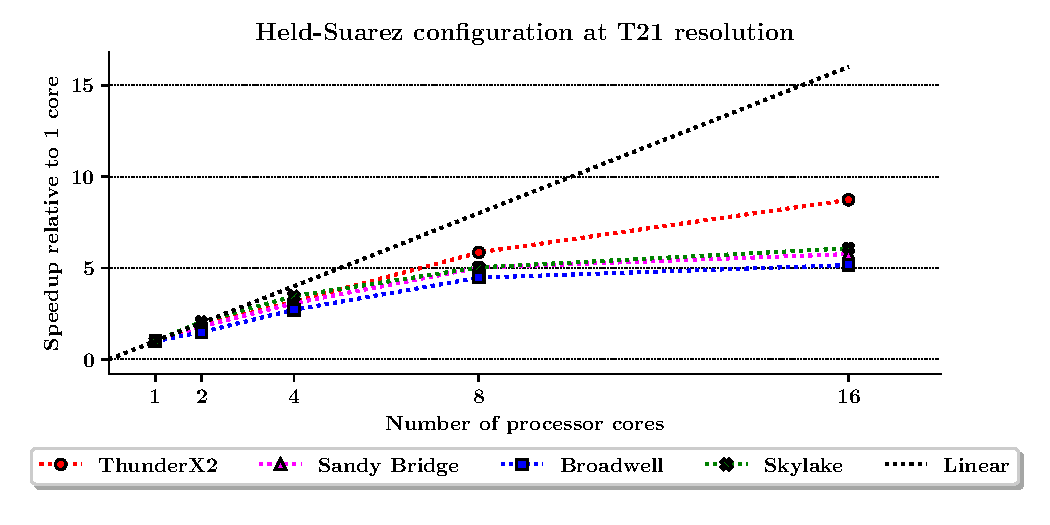
\includegraphics[width=1\textwidth]{img/speedup-T21-Held_suarez.pdf}
\caption[Speedup of the Held-Suarez configuration at T21 resolution]{Parallel speedup relative to serial performance for the Held-Suarez configuration running at T21 resolution.}
\label{fig:t21-scale}
\end{center}
\end{figure}
\par
When Isca is run on 8 cores the Sandy Bridge, Broadwell and Skylake processors see a performance improvement of  5.1$\times$, 4.5$\times$ and 5.0$\times$ relative to the serial runtime, respectively, before plateauing between 8 and 16 processor cores (Figure \ref{fig:t21-scale}). The ThunderX2 speeds up by 5.9$\times$ when run on 8 cores, and 8.7$\times$ when run on 16 cores. When increasing the number of processor cores from 8 to 16 for the Held-Suarez configuration, there is only an approximate 1.15$\times$ performance gain for the Intel processors. This is typical of many parallel codes, whereby the performance benefit of additional compute resources decreases as more processor cores are utilised \cite{asanovic2006landscape}. As this problem size is small, more time is spent in communication relative to compute when a greater number of processor cores are used. 
\par

\begin{figure}[htbp]
\begin{center}
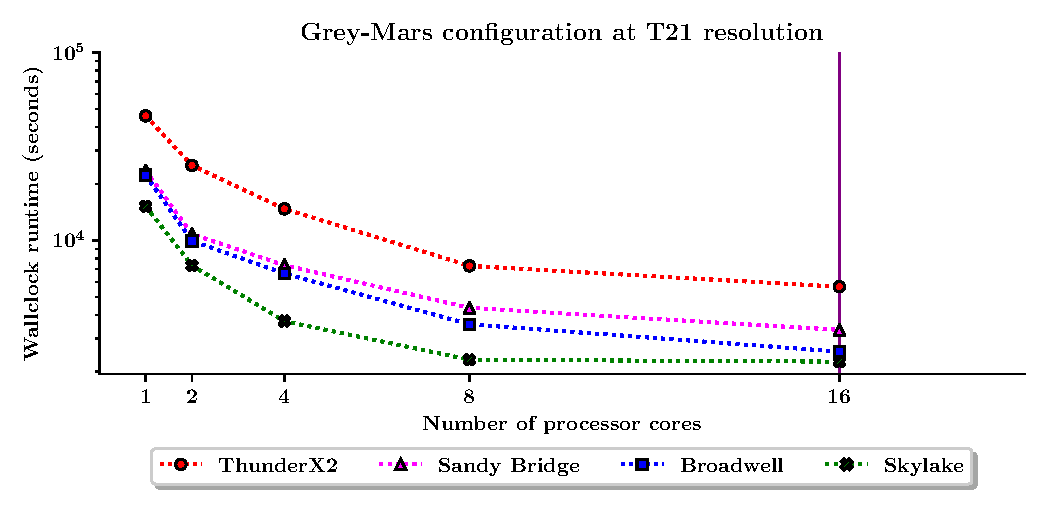
\includegraphics[width=1\linewidth]{img/scaling_graph_T21_Grey_mars.pdf}
\caption[Wallclock runtime of the Grey-Mars configuration at T21 resolution]{Wallclock runtime of the Grey-Mars configuration running at T21 resolution across all processor architectures.}
\label{fig:t21-scale-grey}
\end{center}
\end{figure}
\newpage


The scaling curve in Figure \ref{fig:t21-scale-grey} shows a sublinear plateau for all node configurations, whereby the wallclock runtime of all four processors reduces steadily from 1 to 8 processor cores. The wallclock runtime is greatest when the program is run in serial and lowest when run on 16 cores, which is the maximum number of cores possible for this resolution. The trend observed for the Grey-Mars configuration (Figure \ref{fig:t21-scale-grey}) is comparable to that of the Held-Suarez result (Figure \ref{fig:t21-scale}), whereby the slowest runtime is the serial case and the fastest is the 16 core case. The Skylake processor massively outperforms all other processors when run on 8 cores, however it quickly tapers off when run on 16 cores, running just 1.02$\times$ faster than the 8 core case.
\par
%To determine the importance of memory bandwidth at this resolution, the 16 core configuration was rerun on the Broadwell processor. However, the cores were split across two nodes. Figure x shows that...x
\begin{figure}[htbp]
\begin{center}
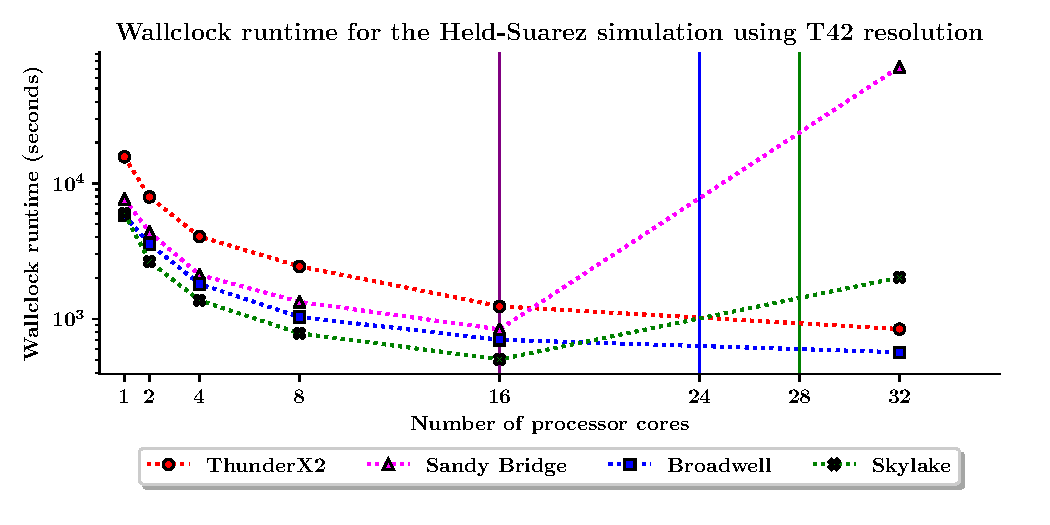
\includegraphics[width=1\textwidth]{img/scaling_graph_T42_Held_suarez.pdf}
\caption[Wallclock runtime of the Held-Suarez configuration running at T42 resolution]{Wallclock runtime of the Held-Suarez configuration running at T42 resolution across all processor architectures.}
\label{fig:t42-scale}
\end{center}
\end{figure}

\newpage
%T42 discussion
%\subsection{T42 resolution}
\begin{figure}[htbp]
\begin{center}
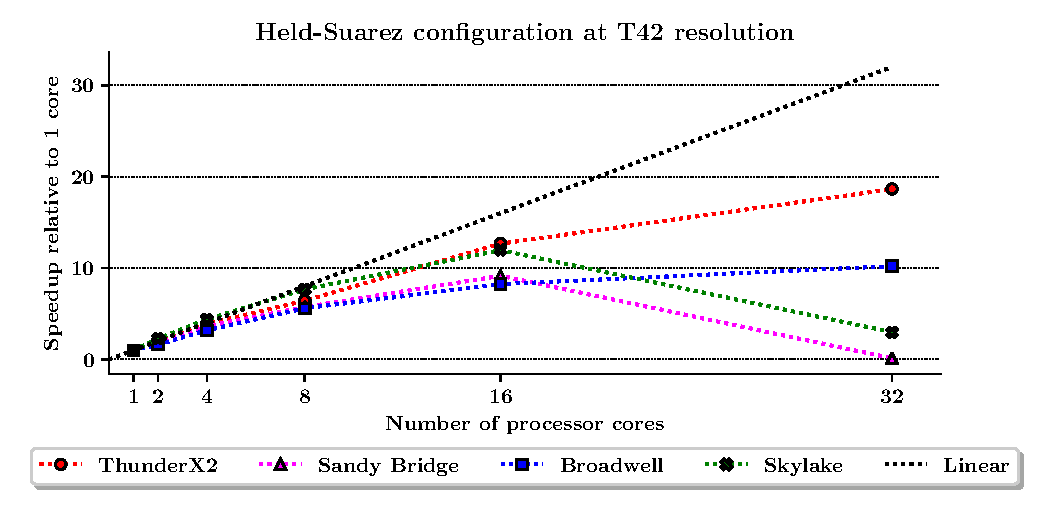
\includegraphics[width=1\linewidth]{img/speedup-T42-Held_suarez.pdf}
\caption[Speedup of the Held-Suarez configuration at T42 resolution]{Speedup of the Held-Suarez configuration running at T42 resolution relative to serial runtime across all processor architectures.}
\label{fig:held-t42-speedup}
\end{center}
\end{figure}
Increasing the spatial resolution to T42 (Figures \ref{fig:t42-scale}, \ref{fig:held-t42-speedup} ) presents a similar scaling curve to that observed for the T21 resolution (Figure \ref{fig:t21-scale-grey}). For all processors except Sandy Bridge, the slowest runtime is measured for the serial code and the performance improves until the program is run on 16 cores. For the Intel processors, running on more than 16 cores requires multiple nodes, which has a dramatic impact on the performance of the Sandy Bridge and Skylake processors. At 32 cores the performance of the Sandy Bridge and Skylake processors reduces from 9.2$\times$ to 0.1$\times$ and 12.0$\times$ to 3.0$\times$, respectively. The Broadwell and ThunderX2 processors improve at this core count, from 8.2$\times$ to 10.2$\times$ and 12.7$\times$ to 18.7$\times$, respectively. Although the ThunderX2 does not provide the fastest overall runtime (Figure \ref{fig:t42-scale}), plotting the speedup relative to the serial runtime demonstrates that it exhibits the best level of scaling (Figure \ref{fig:held-t42-speedup}). This can be attributed to the large core count of the processor, which means that it does not have to rely on internode communication. 
\begin{figure}[htbp]
\begin{center}
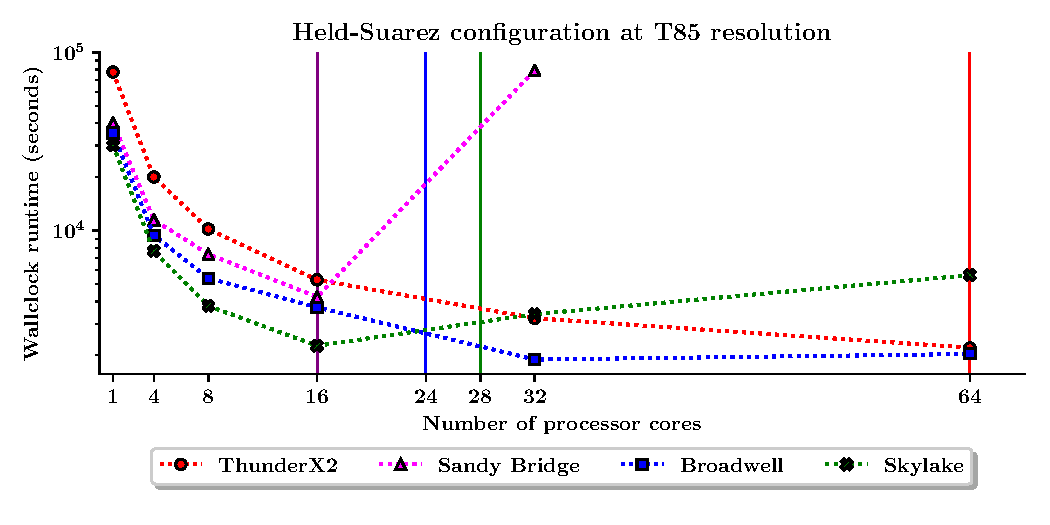
\includegraphics[width=0.94\textwidth]{img/scaling_graph_T85_Held_suarez.pdf}
\caption[Wallclock runtime of the Held-Suarez configuration at T85 resolution]{Wallclock runtime of the Held-Suarez configuration running at T85 resolution across all processor architectures.}
\label{fig:t85-scale}
\end{center}
\end{figure}


\par

%T85 discussion
%\subsubsection{T85 resolution}


\par
\begin{figure}[htbp]
\begin{center}
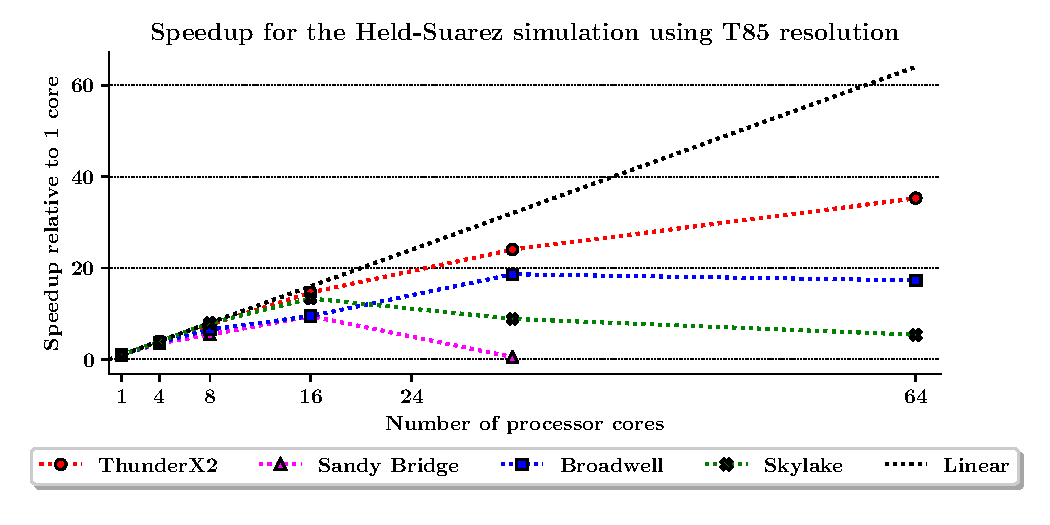
\includegraphics[width=1\textwidth]{img/speedup-T85-Held_suarez.pdf}
\caption[Speedup of the Held-Suarez configuration at T85 resolution]{Speedup of the Held-Suarez configuration running at T85 resolution relative to serial runtime across all processor architectures.}
\label{fig:t85-speedup}
\end{center}
\end{figure}
\par	
For the T85 resolution (Figures \ref{fig:t85-scale} and \ref{fig:t85-speedup}), the performance of the Broadwell processor begins to decline when run on 64 cores across three nodes, reducing from a 18.6$\times$ speedup at 32 cores to a 17.3$\times$ speedup at 64 cores (Figures  and \ref{fig:t85-scale}). This suggests that this is the point at which the cost of communication outweighs the benefit of additional parallelism for this processor. The performance of the ThunderX2 continues to improve when run on 64 cores, increasing from 24.0$\times$ at 32 cores to 35.3$\times$ at 64 cores.

\subsection{Conclusions and discussion}
This scaling study highlighted some of the architectural differences between Intel and Arm processors. Arm's approach to processor design relies on a greater number of simple processor cores, in comparison to Intel's fewer, more complex cores. This design complemented the Isca code by keeping communication inside a single node for resolutions of T85 and below, allowing for competitive runtimes to that of the Intel processors. 
\par
MPI is primarily used for communication between nodes, however messages are exchanged using shared memory when used within a single node \cite{mpi2015standard}. This can greatly reduce the amount of time spent on communication as there is no data transfer between nodes, which can be an expensive process. This is likely what is causing Isca to scale well on the ThunderX2. In contrast, memory-bandwidth bound codes can see significant gains to performance when run on multiple nodes, which increases the total memory bandwidth and therefore reduces the cache-contention between processors \cite{milfeld2014hpc}.
\par
The performance of the Intel processors suffered when run on multiple nodes. This is to be expected on the Skylake nodes as the \gls{bp} supercomputer does not have a high-speed interconnect, using only ethernet to connect compute nodes. Interestingly, the lowest performance observed for the dual-node configuration is the Sandy Bridge processor, which takes 82$\times$ longer to complete the same job than when running on a single node. \gls{bcp3} uses QDR InfiniBand, which has a theoretical throughput of 8 GB/s per connection and should therefore not exhibit this behaviour \cite{grun2010introduction}. The Sandy Bridge node was the only Intel configuration to use OpenMPI instead of Intel MPI. Unlike Intel MPI, OpenMPI has not been developed specifically for Intel compute nodes, and this could have affected the internode performance for this configuration. However, it is unlikely that this is the sole reason for the poor internode performance. Both the ThunderX2 and Broadwell processors do not exhibit this behaviour when run on 32 and 64 cores, which suggests that the issue is most likely caused by internode communication rather than a bug in the model that manifests at higher core counts.
\par
Due to restrictions imposed by domain decomposition, the Grey-Mars configuration cannot be run at resolutions higher than T42. Because of this, the results for the T85 resolution are limited to the Held-Suarez configuration only. Additionally, the time limit imposed by the queuing system prevented results from being gathered for the Sandy Bridge processor when running on 64 cores as the runtime was greater than 360 hours, which is the longest amount of time available for a single job on the BCP3 supercomputer.
%\begin{itemize}
%\item BluePebble is slow because it just uses ethernet. 
%
%\item Athough MPI is used, most of the comms will happen inside shared memory as MPI is not stupid. 
%
%\item It would be interesting to run the model at much higher resolutions to see how it reacts to processors at very high core counts.
%
%\item Generally, running on a greater number of nodes improves the performance of codes that are bound by memory bandwidth, as a greater number of nodes implies a larger memory bandwidth. Although the ThunderX2 has the largest memory bandwidth, it does not have the best runtime at all resolutions. 
%
%\end{itemize}



\section{Experiment B: Compiler comparison}
This experiment measured the wallclock runtime of Isca when complied using the ICC, GCC and CCE compilers using two different model configurations and resolutions (Tables \ref{tbl:compilers} and \ref{tbl:-compiler-cores}). 

\subsection{Results}
For all configurations tested on Intel nodes ICC outperformed GCC (Figure \ref{fig:compiler-comparison-t42}). ICC provides a mean performance improvement of 1.26$\times$ over GCC across both the T21 and T42 resolutions. On the ThunderX2, GCC was 1.4$\times$ faster than CCE at the T21 resolution but just 1.01$\times$ faster at the T42 resolution.


\par
\begin{figure}[htbp]
\begin{center}
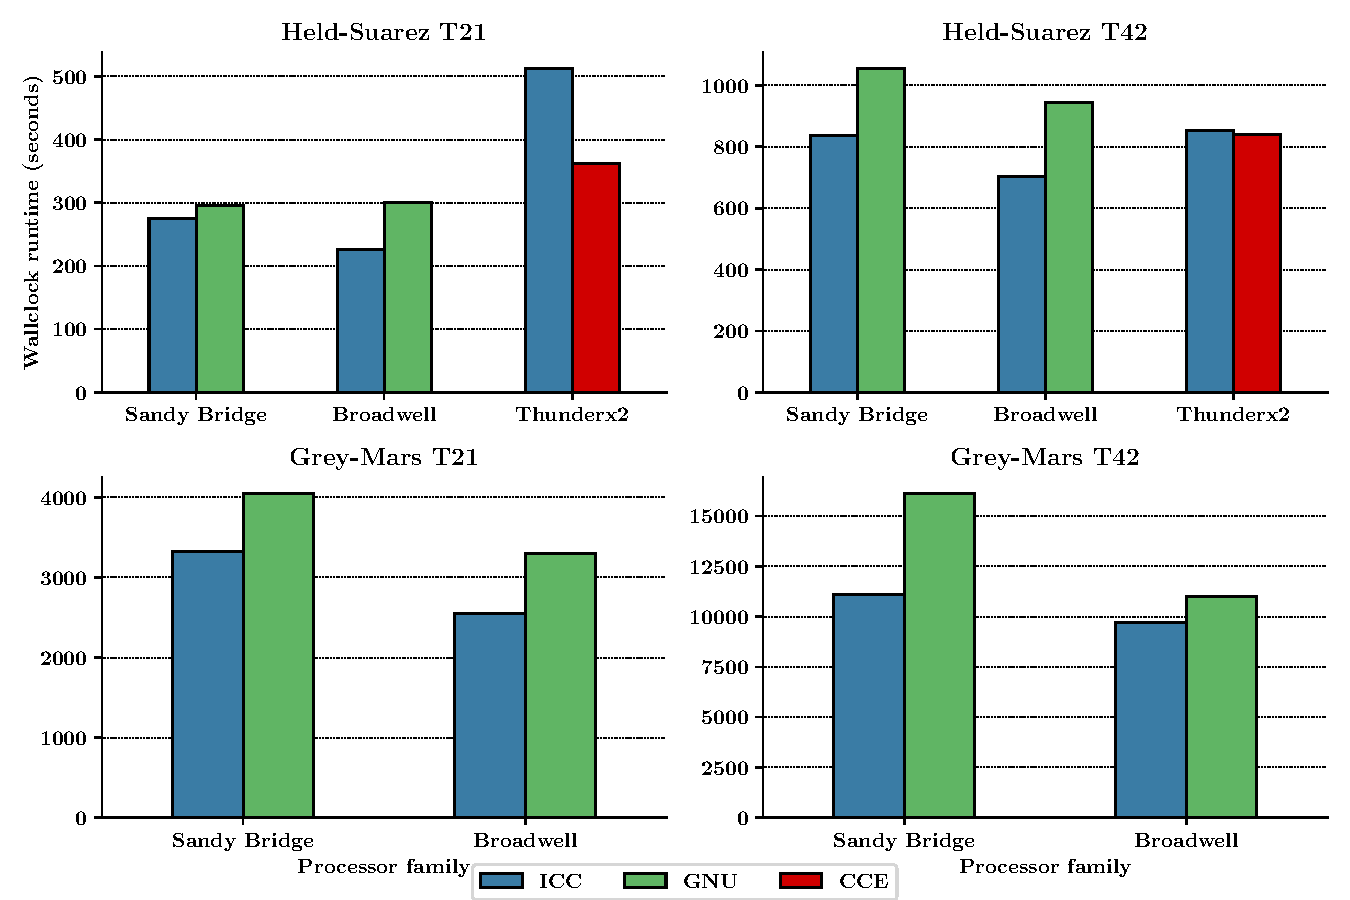
\includegraphics[width=1\textwidth]{img/compiler-comparison.pdf}
\caption[Performance comparison using different compilers]{Runtimes for the Held-Suarez and Grey-Mars configurations using different compilers.}
\label{fig:compiler-comparison-t42}
\end{center}
\end{figure}
\subsection{Conclusions and discussion}
It can be expected that ICC outperforms GCC on Intel hardware as Intel develops their compilers alongside their processors. Consequently, the Intel compilers produce well-optimised instructions for the architecture. This experiment confirmed this expectation as ICC outperformed GCC in all cases. For the ThunderX2, GCC outperformed CCE. For both compilers, flags were specified to produce hardware specific instructions for the ThunderX2 processor, however neither compiler has been exclusively developed for the Armv8 architecture. Therefore, this performance difference could be explained by the the maturity of GCC in comparison to CCE as the compiler has been in constant development since 1987, however there is no evidence to support this claim. 


\section{Experiment C: Vectorisation analysis}
This experiment measured the performance speedup of Isca when the model was compiled to use SIMD instructions, compared to when run in scalar.
\subsection{Results}
\begin{figure}[htbp]
\begin{center}
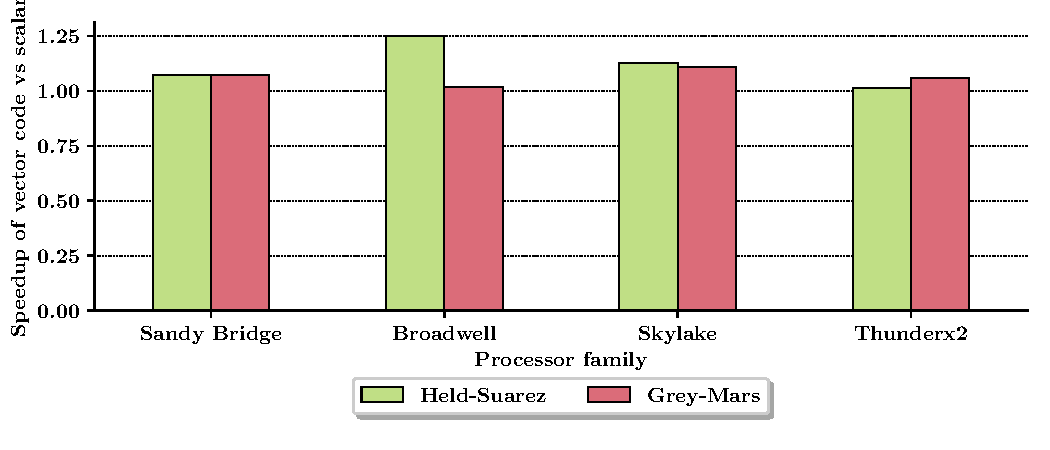
\includegraphics[width=0.9\textwidth]{img/speedup-vector.pdf}
\caption{Speedup of the vectorised code relative to scalar. }
\label{fig:vector-gains}
\end{center}
\end{figure}
\par
Only marginal performance gains are observed when running Isca using SIMD instructions compared to scalar (Figure \ref{fig:vector-gains}). For the Held-Suarez model there is a 1.07$\times$, 1.25$\times$, 1.13$\times$ and 1.01$\times$ performance improvement for the Sandy Bridge, Broadwell, Skylake and ThunderX2 processors, respectively. For the Grey-Mars configuration there is a 1.07$\times$, 1.02$\times$, 1.11$\times$ and 1.06$\times$ performance improvement for the same processors.

\subsection{Conclusions and discussion}
Some of the most time-consuming compute kernels in Isca operate over arrays of double-precision complex numbers. In the Fortran programming language a complex number is composed of a pair of floating point numbers, representing both real and imaginary parts of the complex number. This means that a double-precision complex number of kind 8 uses 128 bits of memory; both real and imaginary parts of the number are a real value of 8 bytes each. This means that vectorisation is costly in parts of the code that iterate over complex data structures, and impossible on the 128-bit registers used in Intels SSE, and Arms NEON SIMD extensions. Interestingly, Intel's cost model often determines that there is no benefit to using SIMD instructions on arrays of double-precision complex numbers, even when 256-bit and 512-bit registers are available as a results of AVX-2 and AVX-512, respectively.
\par
Small but consistent performance gains were measured when the model was compiled to use SIMD instructions. This suggests that the model is not heavily dependant on vectorisation to provide performance. For the Held-Suarez configuration the ThunderX2 saw the least improvement, which was expected as the ThunderX2 only has 128-bit vector registers. Following the ThunderX2 was the Sandy Bridge processor, which uses the AVX instruction set. Although this allows for a vector width of up to 256-bits it does not include fused multiply-accumulate operations like the AVX-2 instructions used by Broadwell and the AVX-512 instructions used by Skylake, and this is reflected by its performance \cite{reinders2013intel, intel2017avx}.



\section{Experiment D: Computation rate}
Section \ref{sec:app-benchmarking} defines CCPG as the cost of computing a single grid cell per time step of the simulation. This experiment measures the cost of computation relative to the number of concurrently utilised processors. %When run in serial, 100\% of the program runtime is spent on compute as there is no communication between processors. 
\label{sec:comm-analysis}
\subsection{Results}
\begin{figure}[htbp]
\begin{center}
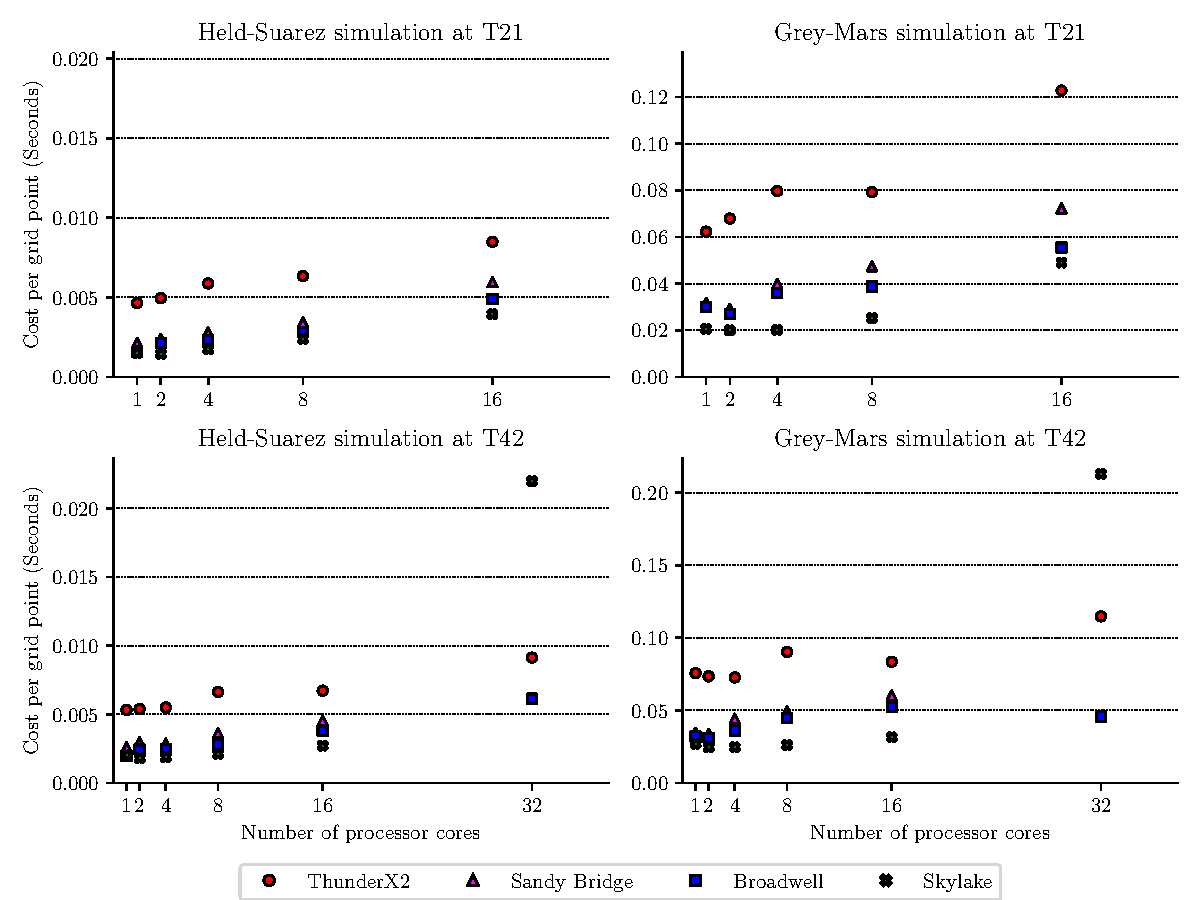
\includegraphics[width=1\textwidth]{img/cost-per-grid-point.pdf} 
\caption[Cost per grid point at T21 and T42 resoltuions]{Cost per grid point for the Held-Suarez and Grey-Mars configurations at T21 and T42 resolutions.}
\label{fig:cost-per-grid-point}
\end{center}
\end{figure}
For the Held-Suarez configuration running at the T21 resolution the introduction of parallelism causes an increase in \gls{ccpgpt} for all node configurations except Skylake (Figure \ref{fig:cost-per-grid-point}). The \gls{ccpgpt} decreased for the Skylake node when parallelism was introduced to the model. Increasing the amount of parallelism past the utilisation of two cores causes the \gls{ccpgpt} to increase almost linearly for all processors at this resolution. The same trend was observed for the Held-Suarez configuration when running at the T42 resolution. However, for the dual-node case the \gls{ccpgpt} sharply increases for the Skylake node with a cost 6.7$\times$ greater than when run on the maximum capacity of a single node.
\par
For Intel nodes running the Grey-Mars configuration at the T21 resolution, the CPPG initially decreases when parallelism is introduced. However, running on more than 4 processor cores increases the \gls{ccpgpt}. This is not the case for the ThunderX2, for which the \gls{ccpgpt} increases until it is run on 8 processor cores at which a plateau is reached, before increasing again at 32 cores. This same pattern is observed for the Grey-Mars configuration running at the T42 resolution, however the \gls{ccpgpt} dips for the ThunderX2 when run on 16 cores, rather than reaching a plateau. 

\subsection{Conclusions and discussion}
Plotting the \gls{ccpgpt} demonstrates that increasing the number of processors also increases the cost to compute a single grid point (Figure \ref{fig:cost-per-grid-point}). Although there are more processors collectively working on the problem, a greater portion of the runtime is spent on communication and therefore processors spend more time idle. Although increasing the amount of parallelism causes the overall wallclock runtime to decrease, the total CPU time increases, which indicates that the code is less efficient. 

\section{Experiment E: Time spent in the MPI library}
\label{sec:mpi-comms}
This experiment measured the percentage of runtime spent in the MPI library and the communication time between processors for a single epoch of an Isca experiment running at T42 resolution.

\subsection{Results}
\begin{figure}[htbp]
\begin{center}
	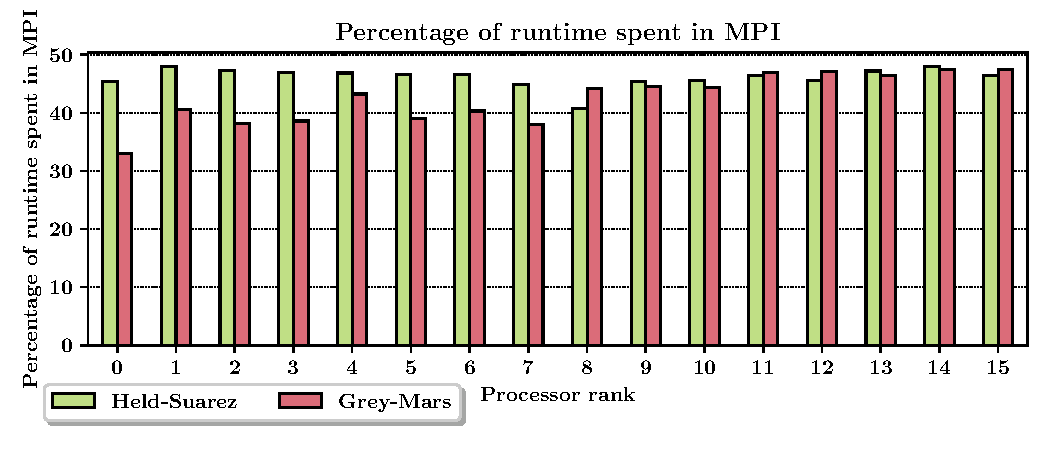
\includegraphics[width=0.9\textwidth]{img/mpi-barrier-time.pdf}
\caption[Percentage of runtime spent in MPI across processes]{Percentage of runtime spent in MPI across individual process ranks for both the Held-Suarez and Grey-Mars model configurations.}
\label{fig:mpi-barrier}
\end{center}
\end{figure}
For the Held-Suarez configuration each process spends between 40.8\% and 48.1\% of its total runtime in calls to MPI, and no discernible patterns can be identified through visual inspection of Figure \ref{fig:mpi-barrier}. For the Grey-Mars configuration each process spends between 33.0\% and 47.5\% of its total runtime in calls to MPI. Processes 0-7 spend a much smaller percentage of their runtime in calls to MPI in comparison to processes 8-15, and process 0 spends a significantly smaller percentage of runtime in calls to MPI than any other process. Additionally, the time spent in the MPI library generally increases relative to the processor rank number. 
\par
\begin{figure}[htbp]
\begin{center}
%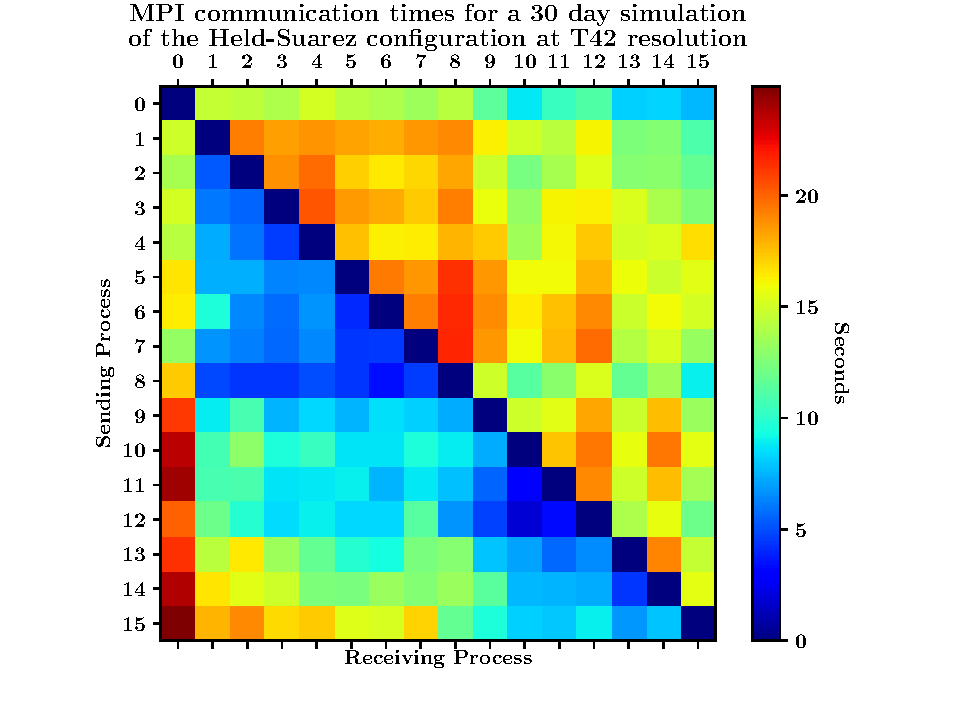
\includegraphics[width=0.49\textwidth]{img/comm_mat_Held-Suarez.pdf}
\includegraphics[width=1\textwidth]{img/comm_mat_grey-mars.pdf}
\caption[Communication matrix for the Grey-Mars model configuration]{Communication matrix for the Grey-Mars model configuration when run at the T42 resolution. Communication time has been measured as the sum of all time spent inside the MPI library.}
\label{fig:comm_mat}
\end{center}
\end{figure}
\par
The longest communication times are measured when processes 8-15 transmit data to process 0, with a mean communication time of 118.5 seconds (Figure \ref{fig:comm_mat}). However, process 0 has the lowest sending times of any process, with a mean communication time of just 31.3 seconds. This suggests that process 0 is consistently taking the longest amount of time to reach points of synchronisation and can exchange data almost immediately upon reaching MPI barriers. 

\subsection{Conclusions and discussion}
Load imbalance refers to an uneven distribution of work across compute resources. In the domain of HPC it affects the performance of parallel codes only. For Isca, the large variation in MPI time observed across processor ranks suggests that the model suffers from a significant load balancing issue, which is amplified by the large portion of runtime that is spent inside calls to MPI.
\par
Many of the subroutines found in Isca with long execution times inherently involve expensive communication. For example, when calculating global sums over 2D fields, each processor gathers the missing pieces of data they require to construct the global field from all other processes using blocking communication \cite{schmidt2007benchmark}. As Isca operates on a global domain, these points of synchronisation are unavoidable as communication must finish between all processes before the program can continue. Subroutines like this are found all throughout the Isca code, and each contributes to the large amount of time the model spends on communication. Unfortunately, Isca has been built around these points of synchronisation, and optimisation is not possible by using asynchronous message passing without affecting the scientific validity of the model. 
\par
Referring back to Figure \ref{fig:mpi-barrier}, the Held-Suarez configuration generally presents more consistency amongst its processors than the Grey-Mars configuration, which is to be expected as the forcing component of the model means that the calculations are more consistent on each rank. Although some variation was measured in MPI time across processor ranks for the Held-Suarez model configuration, this can be attributed to environmental variables outside the control of the experiment. The Grey-Mars simulation exhibits more severe symptoms of load imbalance. As discussed in Section \ref{sec:grey-mars-conf}, some radiation models can suffer from a load-balancing issue whereby calculations take longer on the side of the planet facing the Sun. Although Isca 

\par
Check if this is true by running with data from run13. 

\section{Experiment E: Runtime variation}
This experiment measured the differences in runtimes for each individual epoch comprising an Isca simulation.

\subsection{Results}
\begin{figure}[htbp]
\begin{center}
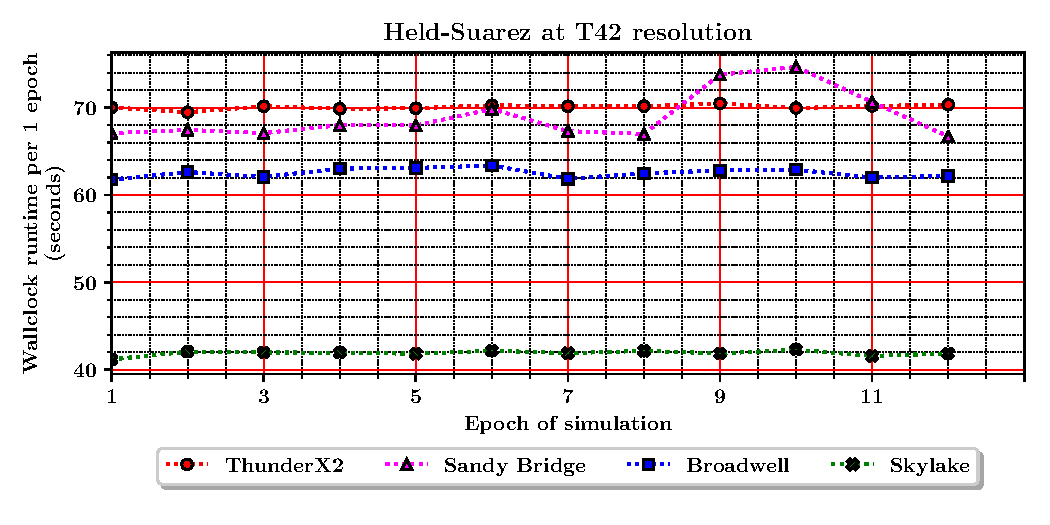
\includegraphics[width=0.8\textwidth]{img/held_suarez-variation.pdf}
\caption{Variation in runtimes for the Held-Suarez configuration running at T42 resolution.}
\label{fig:variation-comparison-held-t42}
\end{center}
\end{figure}
For the Held-Suarez model configuration the runtimes for individual epochs have a range of 0.99 seconds, 1.11 seconds and 1.60 seconds for the ThunderX2, Skylake and Broadwell processors, respectively (Figure \ref{fig:variation-comparison-held-t42}). However, the Sandy Bridge processor had more fluctuations in runtime throughout the full simulation with a range of 7.97 seconds.
\begin{figure}[htbp]
\begin{center}
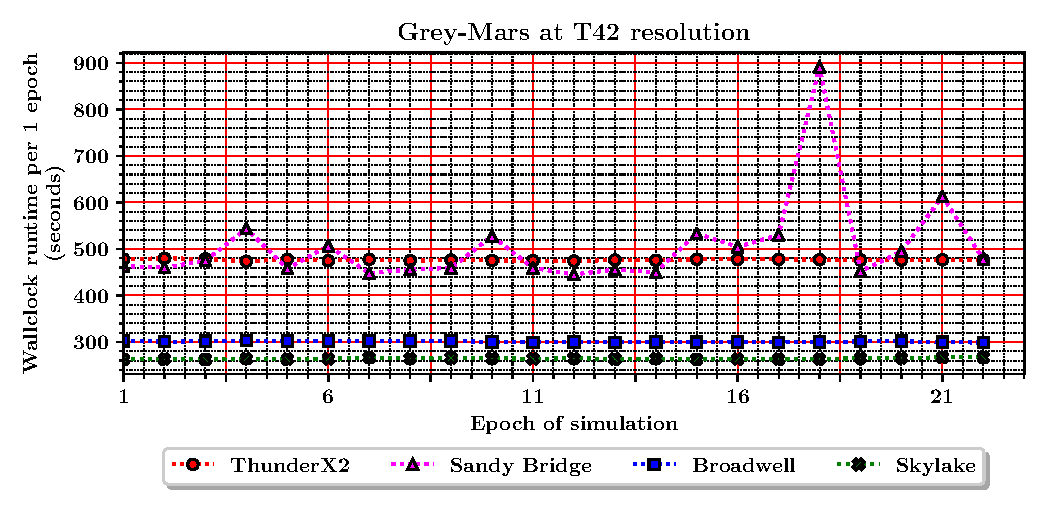
\includegraphics[width=0.8\textwidth]{img/grey_mars-variation.pdf}
\caption{Variation in runtimes for the Grey-Mars configuration running at T42 resolution.}
\label{fig:variation-comparison-mars-t42}
\end{center}
\end{figure}
\par
The Grey-Mars simulation presents similar results, showing only minor variations in epoch runtime across all processors except Sandy Bridge (Figure \ref{fig:variation-comparison-mars-t42}). There is a large peak for the Sandy Bridge processor at epoch 18, however rerunning this experiment causes peaks at seemingly random intervals.

\subsection{Conclusions and discussion}
The FMS Manual warns of a spin-up time that can slow the performance of the first epoch of a simulation due to the initialisation of the global starting state \cite{balaji2002fms}. This effect has not been observed in either the Held-Suarez or Grey-Mars model configurations, even in simulations that have not been visualised in Figures \ref{fig:variation-comparison-held-t42} and \ref{fig:variation-comparison-mars-t42}. The FMS manual was written in 2002 when the clock speeds of high performance processors were in the range of 1.1 GHz to 1.5 GHz, and memory-bandwidth rarely exceeded 1,600 MB/s \cite{behling2001power4, carvalho2002gap}. Perhaps the spin-up cost is now negligible when the model is run on more powerful hardware. 
\par
The runtimes observed on the ThunderX2, Broadwell and Skylake processors indicate that each epoch contains the same amount of work and no part of the planetary orbit is more computationally expensive than others. The results obtained on the Sandy Bridge processor may be attributed to environmental factors, and can therefore be treated as an outlier. 


\section{Experiment F: Roofline model analysis}

\begin{figure}[htbp]
\begin{center}
 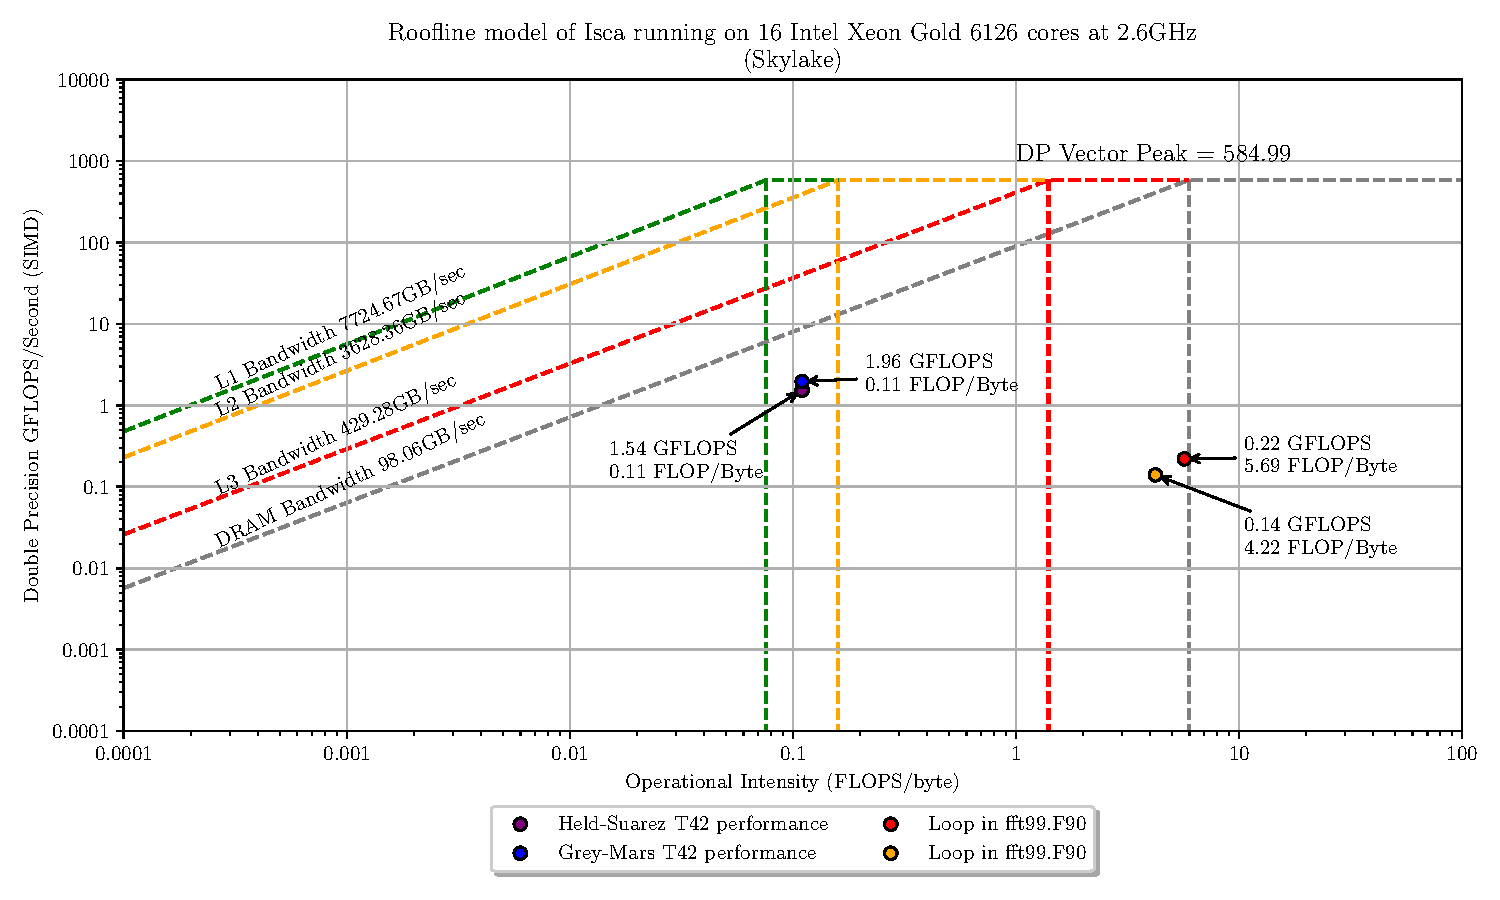
\includegraphics[width=\textwidth]{img/roofline_model_bluepebble.pdf}
\caption[Roofline model of Isca on Intel hardware]{Roofline model for 16 cores of two Intel Xeon Gold processors at 2.6 GHz. } 
\label{fig:roofline}
\end{center}
\end{figure}

The Held-Suarez simulation running at the T42 resolution delivers an operational intensity of 0.11 FLOPS/Byte and a double-precision floating point performance of 1.54 GFLOPS (Figure \ref{fig:roofline}). This indicates that the configuration is limited by memory-bandwidth, as the program total performance is located underneath the DRAM ceiling. The Grey-Mars configuration presents a floating point performance of 1.96 GFLOPS, with the same operational intensity as the Held-Suarez configuration. Intel Advisor suggests that the peak double-precision floating point performance of a code running on the Skylake architecture using SIMD is 584.99 GFLOPS. This means that the Isca code is only running at 0.26\% of the peak performance available on the hardware.

\subsection{Conclusions and discussion}
In addition to quantifying the performance of Isca, Figure \ref{fig:roofline} identifies 2 compute kernels referred to as Loop $x$ and Loop $y$, for optimisation. Loops $x$ and $y$ are both found in Isca's FFT code and provide especially poor floating-point performance of 0.22 GFLOPS and 0.14 GFLOPS, respectively. 
\par
As discussed in Section \ref{sec:spectral-domain}, spectral climate models use a FFT to transform data between the spacial and frequency domains. Isca does this using the \texttt{fft991} subroutine, found in the \texttt{fft99.F90} module. This subroutine is used to perform multiple one-dimensional FFTs in succession over a two-dimensional array of sequential data when converting from a grid-point decomposition to the frequency domain and vice versa. This implementation of the FFT is known as Temperton's FFT, and has been adapted from a Fortran77 code written by Clive Temperton in 1981 \cite{temperton1980fft}. The original source code of this implementation can be found in the deprecated EMOSLIB library by The European Centre for Medium-Range Weather Forecasts \cite{ecmwf2015emoslib}.
\par
\begin{figure}[htbp]
\centering
\begin{subfigure}[b]{1\textwidth}
\centering
   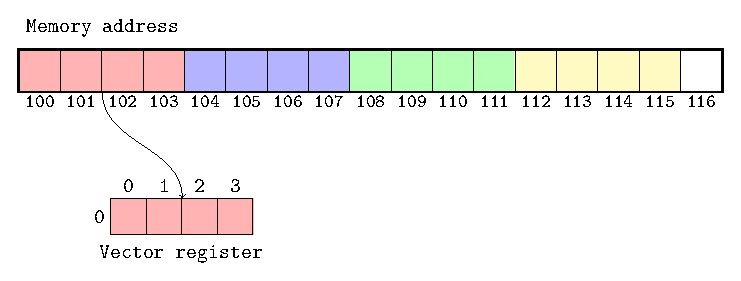
\includegraphics[width=0.9\linewidth]{img/tikz-img/vector_registers_contiguous/vector_registers.pdf}
   \caption{}
   \label{fig:Ng1} 
\end{subfigure}
\end{figure}

\begin{figure}[htbp]\ContinuedFloat

\begin{subfigure}[b]{1\textwidth}
\centering
   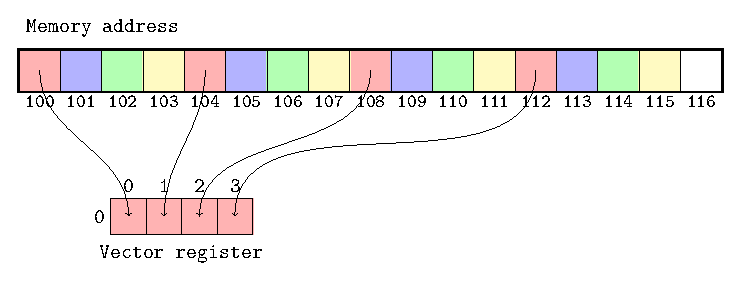
\includegraphics[width=0.9\linewidth]{img/tikz-img/vector_registers_noncontiguous/vector_registers.pdf}
   \caption{}
   \label{fig:Ng2}
\end{subfigure}

\caption[Contiguous and non-contiguous memory access]{ (a) demonstrates that four contiguous single-precision floating point numbers can be read from memory with a single AVX-2 instruction, whilst (b) shows how four separate loads would be required for the same operation for non-contiguous data with a stride of 4.}
\label{fig:vector-registers} 
\end{figure}
\par
Although the \texttt{fft991} subroutine includes preprocessor directives to ignore vector dependencies at the most time-consuming loops neither the Cray, GNU or Intel compilers will perform automatic vectorisation. This results in four loops in the \texttt{fft99.F90} module being run as scalar code, even when vectorisation is possible. Intel Advisor indicates that this is caused by a fixed-width iteration through multiple data structures using a non-contiguous stride, as visualised in Figures \ref{fig:Ng1} and \ref{fig:Ng2}. In the case of the 256-bit wide vector registers found in BCP4's Broadwell processors, eight consecutive floats, or four consecutive doubles, may be loaded from memory with a single AVX-2 instruction. However, if the memory locations are not adjacent then they must be loaded using multiple instructions, negating the benefit of using vector registers. 
\par
\begin{table}[htp]
\caption{Runtime spent inside two compute kernels for both scalar and vector code}
\begin{center}
\begin{tabular}{ c c c }
\toprule 		
Loop						&	Scalar time (milliseconds)	&	Vector time (milliseconds)	\\ 
\midrule
($x$) \texttt{vpassm:1081}		&	822.5				&	649.8				\\
($y$) \texttt{vpassm:1049}		&	793.6				&	459.8				\\
\bottomrule
\end{tabular}
\end{center}
\label{tbl:force-vec}
\end{table}
\par
When forcing the compiler to use SIMD instructions for loops $a$ and $b$ by using the \texttt{!DIR\$ VECTOR ALWAYS} preprocessor directive there is only a marginal performance improvement over the scalar code, (Table \ref{tbl:force-vec}). This supports the hypothesis that the code has not been written to vectorise on modern hardware. 
\par
Another issue regarding Temperton's FFT is that it performs the transformation in place. Although this reduces memory consumption, it introduces additional algorithmic complexity as the results of intermediate calculations are not written to a temporary array. This may have been important in the late 80s and early 90s when memory was in short supply, however modern processors often have in excess of 18 MB of on-chip cache and reducing memory consumption in this case is not a priority. 


%\section{Performance projection}
%The A64FX processor
%\begin{itemize}
%\item list processor specs
%\item compare specs to Thunderx2
%\item Does the A64fx clock down?
%\end{itemize}
%Using these results, how do I think that the code will perform on the new processors?


\section{Summary}
The main observations of all experiments are summarised:
\begin{description}

	\item[Scalability] For the T21 and T42 resolutions, the Skylake processor presents the best level of single-node performance. However, the large core count of the ThunderX2 allows for the best level of single node performance at the T85 resolution. Additionally, the ThunderX2 generally provides the best level of scaling relative to serial performance.

	\item[Load balancing] A serious load balancing issue has been discovered, whereby approximately 40\% of the program runtime is spent inside MPI. Although communication is the biggest performance limiting factor of the code, all identified points of synchronisation are unavoidable, and cannot be optimised without rewriting the entirety of the model.
	
	\item[Vectorisation] As Isca operates on double-precision floating point values, the small vector registers of the ThunderX2 cannot be used on complex numbers. This also affects the performance of the Intel processors, as vectorisation only accounts for a performance gain of between 1.02$\times$ and 1.25$\times$ the scalar code. 
	
	\item[Compilers] On the Intel machines ICC outperforms GCC in all cases, however on the ThunderX2 GCC provides better performance than CCE. These results were used to inform the choice of compiler for all other experiments. 
	
	\item[Slow FFT] Isca uses a FFT that was written in 1981 and it has been demonstrated that some of this code does not automatically vectorise and only insignificant performance gains are observed when forcing the code to use SIMD registers. It has been determined that this is an area of the code that can be optimised. 
	
%	Some of the code responsible for performing a FFT is not vectorising and is based on a 38 year oldTemperton's FFT used by Isca is underperforming  as the code does not vectorise on  partly because the code does not vectorison  Fourier transform code is slow. 
	
\end{description}






% - - - - - - - - - - - - - - - - - - - - - - - - - - - - - - - - - -
% Chapter - Performance Analysis and Optimisation 
% - - - - - - - - - - - - - - - - - - - - - - - - - - - - - - - - - -
\let\textcircled=\pgftextcircled
\chapter[Optimisation]{Optimisation}
\label{chap:optimiations}
This chapter builds upon the findings presented in chapter 7 by describing the design and implementation of two performance optimisations, $A$ and $B$. Optimisation $A$ utilises the FFTW library in place of Temperton's FFT, and optimisation $B$ uses single-precision floating point numbers. 
%These optimisations have been evaluated to ensure they provide a significant performance improvement, whilst retain the scientific validity of Isca.

% FFT Optimisation
\section[FFT optimisation]{Optimisation $A$: Fast Fourier Transform}
Although it may be possible to rewrite Temperton's FFT to efficiently use vector registers, this would be a time-consuming task and does not guarantee a performance improvement. Therefore, the Isca codebase has been modified to allow for the use of the open source \gls{fftw} library instead.



\subsection{Implementation}
In order to call FFTW rather than Temperton's FFT, a new Fortran module \texttt{fftw.F90} has been written. Preprocessor directives have been added to the existing \texttt{fft.F90} file to allow for the type of FFT used by Isca to be selected at compile time. Compiling the model with the \texttt{-DFFTW3} preprocessor directive will compile the model to use \gls{fftw} instead of the default call to Temperton's FFT. Isambard, \gls{bcp3}, \gls{bcp4} and \gls{bp} have module files that allow for automatic linking to the FFTW library. If using the library on other systems the FFTW library must be installed and linked to Isca manually. FFTW provides both a single and double-precision version of its library, with subtle differences to the names of the interfaces it provides. Preprocessor directives must be used to choose which version of FFTW is linked to the Isca code at compile time. 
\par
\begin{figure}[htbp]
\begin{center}
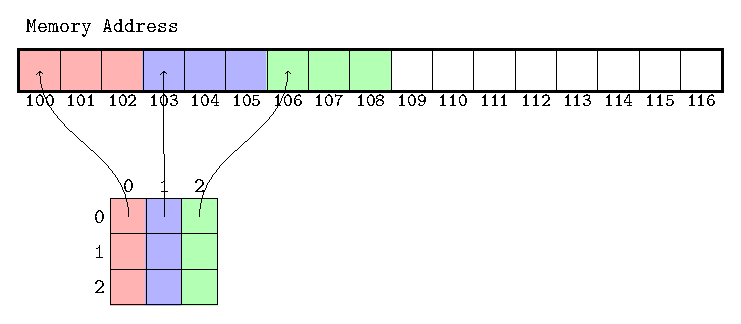
\includegraphics[width=0.9\textwidth]{img/tikz-img/data_layout/data_layout.pdf}
\caption[Two-dimensional data layout in Fortran]{Contiguous data layout in memory for a two-dimensional array in Fortran.}
\label{fig:memalign}
\end{center}
\end{figure}
\par
To guarantee proper data alignment for SIMD utilisation, the data structures on which the FFT is applied are allocated using the \texttt{fftw\_malloc} subroutine and deallocated using the \texttt{fftw\_free} subroutine, both of which are provided by the FFTW library \cite{frigo2005design}. These subroutines have the same behaviour as the \texttt{allocate} and \texttt{deallocate} subroutines found in the Fortran standard library, however they also call \texttt{memalign} to ensure that the data structures are properly aligned \cite{frigo2003fftw}. Figure \ref{fig:memalign} shows contiguous aligned memory for a two-dimensional array in the Fortran programming language, which uses a row-major order for multidimensional array storage \cite{lahey1994fortran}.
\par
Isca computes the DFT of sequences of both real and complex numbers. A one-dimensional transform from a real array of size $N$ results in a complex array of size $N/2$. When implementing this using FFTW, the same input and output arrays are reused for multiple transforms to take advantage of the FFTW plan data structure. As \gls{fftw} computes an unnormalised \gls{dft}, the result is multiplied by the number of items in the input sequence. This means that the result must be scaled by a factor of $1/N$ after the \gls{dft} is calculated, which adds a small overhead to compute costs in addition to the cost of the DFT.  
\par
Additional overhead costs are incurred when populating the input array for which the DFT will be calculated. Fortran is a pass-by-reference language, which means that arguments are passed to subroutines as a pointer. Before the DFT can be calculated the input array must be populated with the data from the array passed to the wrapper subroutine. Although this involves only one iteration though the array, this can accumulate to a significant amount of runtime when many FFTs are called in succession.

\subsection{Verification of results}
To ensure that FFTW computes the same values as Temperton's FFT, both forward and backward transforms were tested on sequences of known data. The results of this test show that both transforms compute the exact same DFT and IDFT for 30 unique sequences of data. Additionally, computing both the DFT and IDFT of a sequence in succession yields the original sequence upon which the transforms were applied.

\subsection{Performance analysis}

\subsubsection{Methodology}

The time taken to complete a number of one-dimensional FFTs was measured for both FFT implementations in order to compare the performance of FFTW against Temperton's FFT. Each FFT implementation was tested on four different sizes of randomly initialised two-dimensional data structures, similar to those found in Isca. For example, a two-dimensional array of size 128$\times$64 will compute the DFT of 128 one-dimensional arrays of size 64. The sizes of the arrays tested correspond to the different array sizes used for the T21 (64$\times$128), T42 (128$\times$64), T85 (256$\times$128) and T170 (512$\times$256) model resolutions. To emulate the Isca code the test program was compiled using the same compiler flags used to compile Isca. Experimental error was accounted for by computing the mean value of 100 transformations, improving the accuracy of findings and reducing the impact of anomalies.

\subsubsection{Results}

\begin{figure}[htbp]
    \centering
    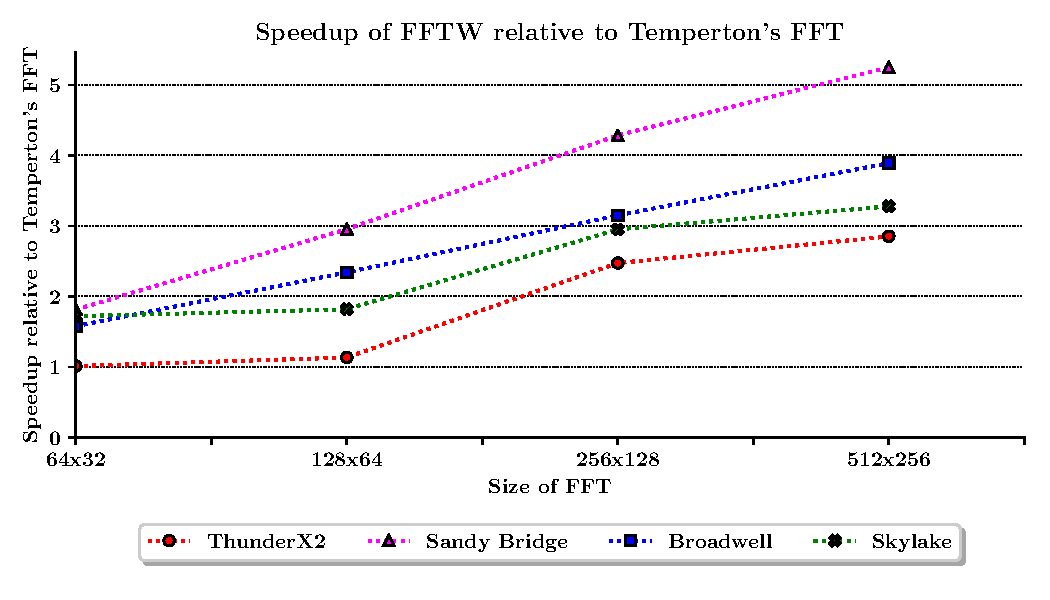
\includegraphics[width=1\textwidth]{img/speedup-fft.pdf}
    \caption[Speedup of FFTW relative to Temperton's FFT]{Speedup of FFTW relative to Temperton's FFT. }
    \label{fig:fft-speedup}
\end{figure}
\par
The performance of both the Sandy Bridge and Broadwell processors improves linearly with the size of the data structure on which the transform is applied (Figure \ref{fig:fft-speedup}). The performance of the ThunderX2 and Skylake processors sharply rises when run on a problem size of 256$\times$128 and 512$\times$256, although only marginal performance gains are observed for the smaller problem sizes. The greatest performance improvement was observed on the Sandy Bridge processor when performing a FFT on a grid size representing the T170 resolution. For this configuration the FFTW code ran 5.25$\times$ quicker than Temperton's FFT, and in all cases the largest problem size saw the greatest performance speedup over Temperton's FFT.
\par
The ThunderX2 had the lowest performance across all problem sizes, and only significant performance gains were observed for problem sizes greater than T42 (Figure \ref{fig:fft-times}). The Intel processors saw the best levels of performance, likely due to the FFTW library originally being written for x86-64 processors. 

\begin{figure}[H]
    \centering
    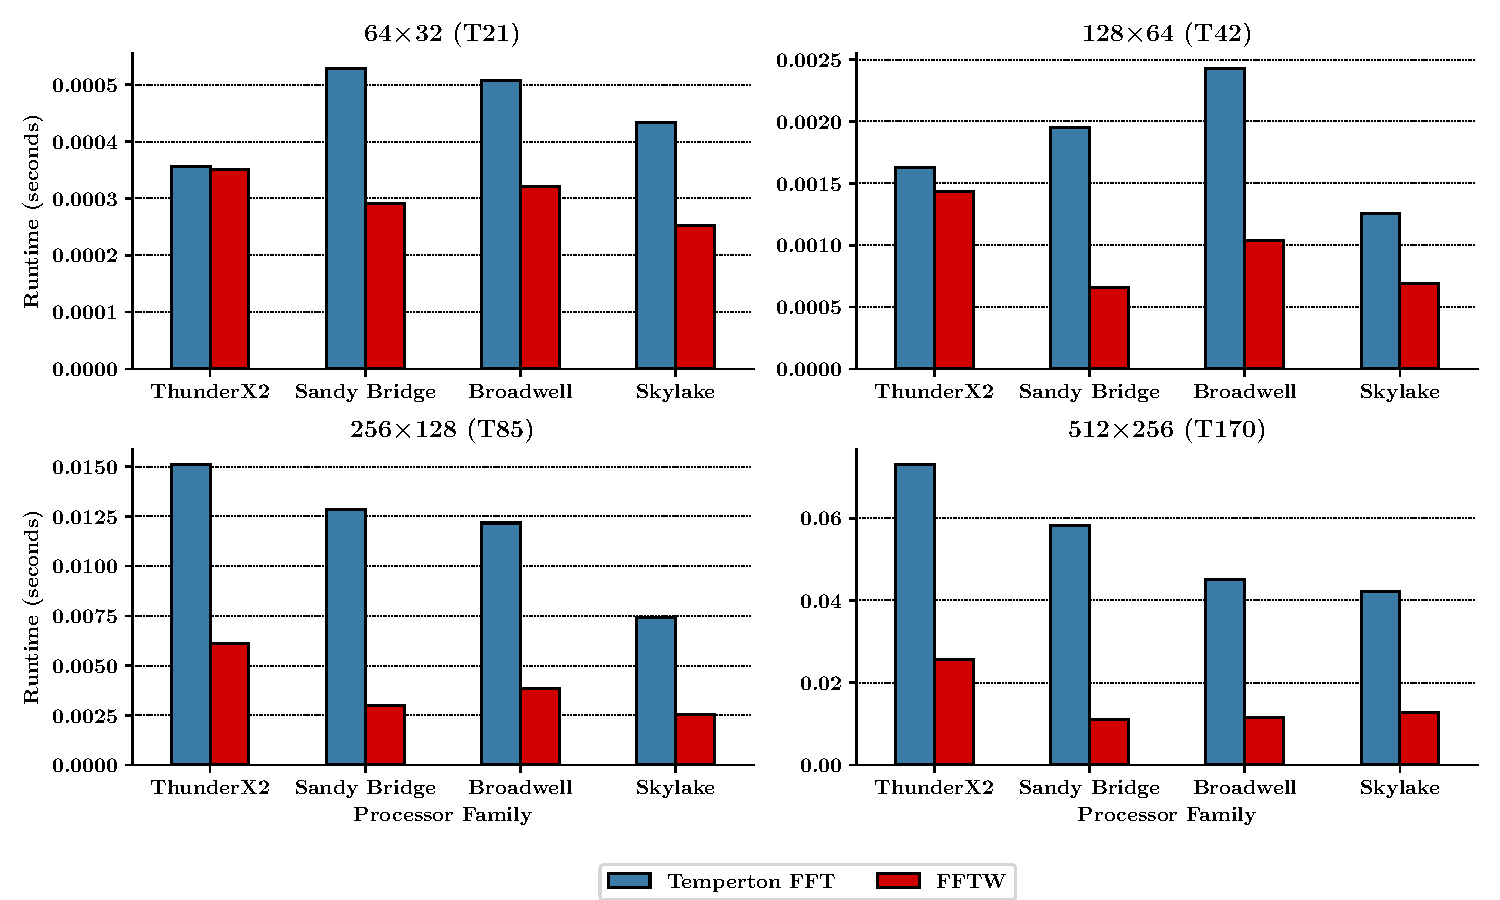
\includegraphics[width=1\textwidth]{img/compare_fft.pdf}
    \caption[Performance comparison of FFTW and Temperton's FFT]{The performance of Temperton's FFT compared to the performance of FFTW across multiple domain sizes.  }
    \label{fig:fft-times}
\end{figure}

\subsubsection{Conclusions and discussion}
Principles of software engineering recommend that code should be modular by design, which means that software components should be separated according to functionality \cite{parnas1972criteria}. Using a library to perform the FFT adheres to this principle and allows for future updates to the library to benefit the performance of Isca. Due to the popularity of the FFTW library, it is under constant development to allow for the utilisation of the latest hardware features, whilst remaining compatible with older systems. 
\par
%Generally, bespoke code does not age well. The findings from these experiment 


%for the modularity of code, which    provides a significant improvement to Its better to use a library that is updated rather than relying on bespoke code that does not evolve with hardware. 
%
%
%so overall this optimisations not. But in terms of the actual FFT its massively quicker.
%Interestingly, the performance gain was only significant on the ThunderX2 for a problem of size 256$\times$128 and greater. 
%\par
%
%\par
%Need to bear in mind that this test was performed on a single processor, so it is expected that the ThunderX2 will have the worst performance. 
%\par

















\section{Optimisation $B$: Single-precision floating point numbers}
\label{sec:floating-pont}
Both x86-64 and AArch64 processors perform scalar floating point arithmetic in 64-bit registers, and therefore the time taken to perform floating point arithmetic on a single data item is approximately the same for both single and double-precision variables \cite{reinders2013intel, aa2011armv8}.   At a larger scale, single-precision arithmetic can improve overall system performance by reducing RAM, cache, and memory bandwidth consumption, in addition to more efficient usage of vector registers \cite{goldberg1991every}.
\par
By default, Isca uses double-precision floating point variables to store all atmospheric variables. As double-precision complex variables in Fortran use 128-bits of memory, SIMD instructions cannot be applied to operations over complex data structures using SSE or NEON registers. To enable complex variables to fit into these registers, Isca has been compiled to use single-precision floating point numbers, halving the memory consumption of complex variables to 64-bits.

\subsection{Implementation}
The Isca code contains existing infrastructure to allow for the default size of real and complex variables to be selected at compile time as the codebase includes interfaces to both single and double-precision versions of subroutines. To change the default size of real and complex variables in the model, a number of preprocessor directives and compiler flags can be specified at compile time to allow for subroutine overloading. This changes the kind of variables declared using the \texttt{MPP\_TYPE\_} macro, which is used throughout the codebase to specify the default kind and type of dummy arguments. 



\subsection{Performance analysis}

\subsubsection{Methodology}
The wallclock runtime of the single-precision version of Isca running both the Held-Suarez and Grey-Mars configurations was measured, allowing for comparison with the double-precision version. Additionally, the operational intensity (FLOPS/Byte) and floating point performance (GFLOPS/s) was remeasured for a single epoch of the program executable. This allowed for a new roofline model to be plotted to visualise how the performance limitations of the code changed. To determine if single-precision variables utilise SIMD registers more efficiently, the runtime of the single-precision version of the model was measured with and without vectorisation enabled. 

\subsubsection{Results}
\begin{figure}[H]
\begin{center}
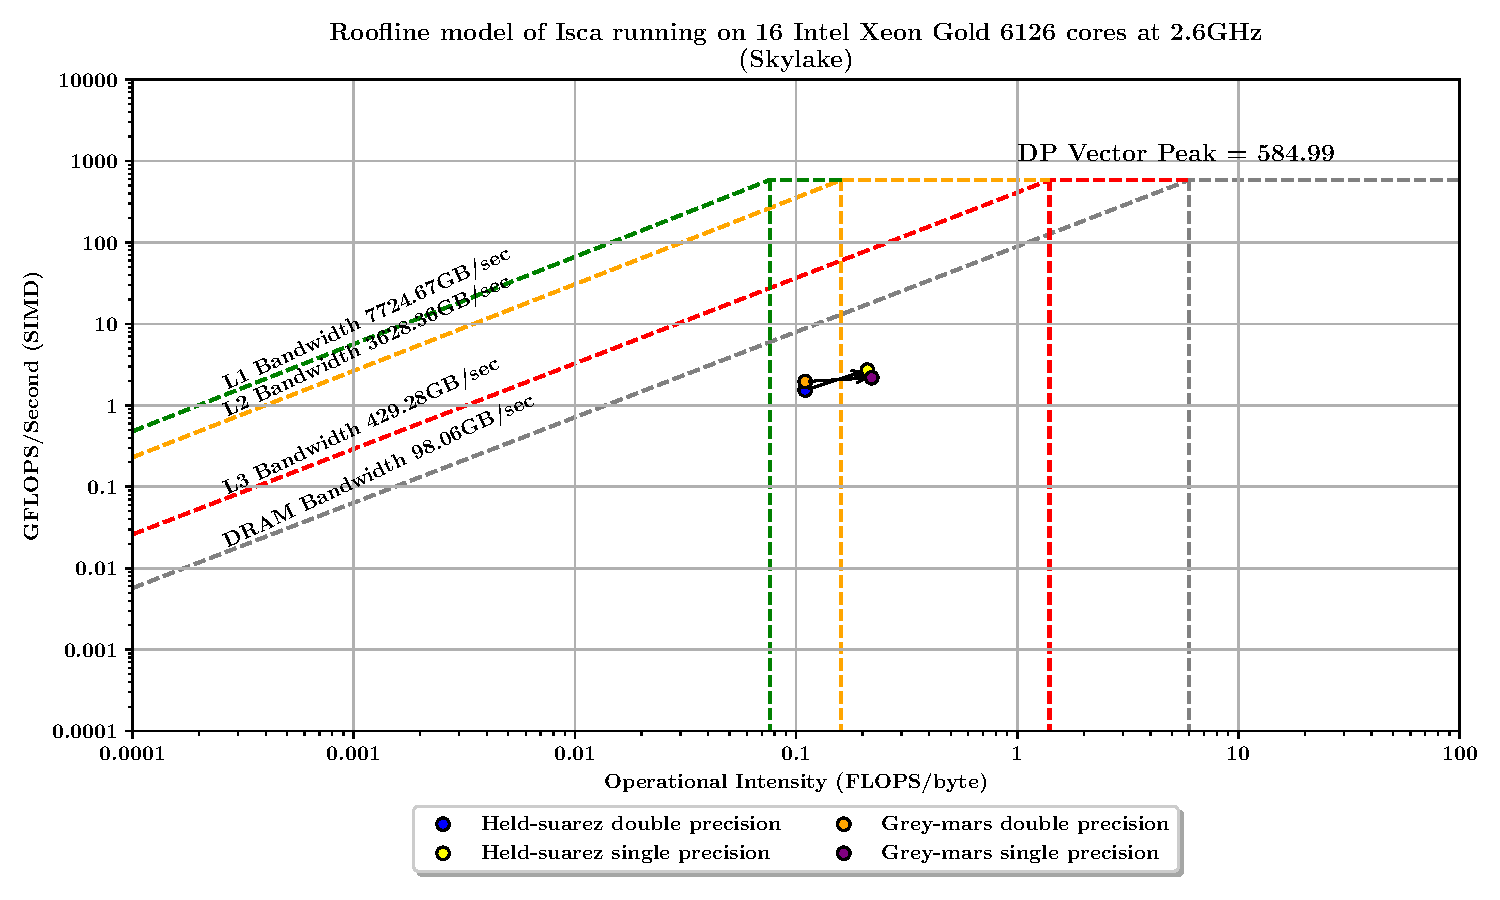
\includegraphics[width=\textwidth]{img/roofline_model_bluepebble_precision.pdf}
\caption[Roofline model comparing single and double-precision arithmetic]{Comparison of the single and double-precision versions of Isca running the Held-Suarez and Grey-Mars model configurations.}
\label{fig:roofline-opt}
\end{center}
\end{figure}
Using single-precision floating point variables, the operational intensity increased from 0.11 to 0.21 for the Held-Suarez configuration, and 0.11 to 0.22 for the Grey-Mars configuration (Figure \ref{fig:roofline-opt}). Additionally, the floating point performance increased from 1.54 GFLOPS to to 2.71 GFLOPS for the Held-Suarez configuration and from 1.96 GFLOPS to 2.18 GFLOPS for the Grey-Mars configuration.

\par
\begin{figure}[H]
\begin{center}
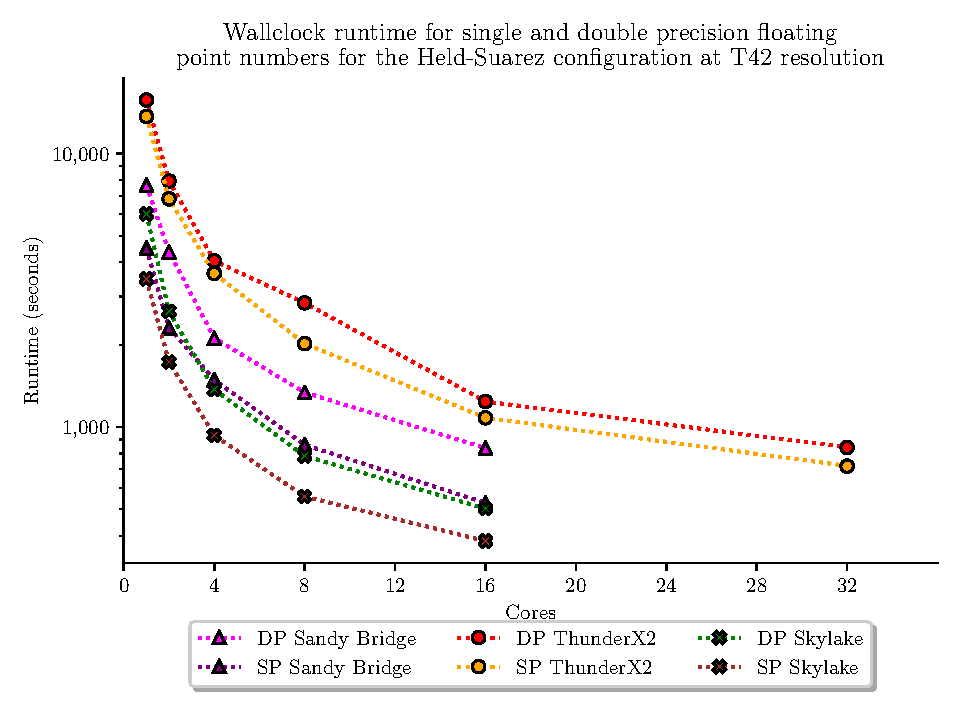
\includegraphics[width=1\textwidth]{img/single-double-precision.pdf}
\caption[Performance comparison of varied precision of floating point numbers]{Comparison of the wallclock runtimes for single and double-precision floating point numbers for the Held-Suarez configuration running at T42 resolution. }
\label{fig:precision}
\end{center}
\end{figure}
\par
Single-precision arithmetic is significantly faster than double-precision arithmetic at all core counts (Figure \ref{fig:precision}). There is no relationship between the level of performance improvement and number of concurrently utilised processor cores, suggesting that the speed of MPI communication is not significantly affected by decreasing the precision of variables.
\par
\begin{figure}[htbp]
\begin{center}
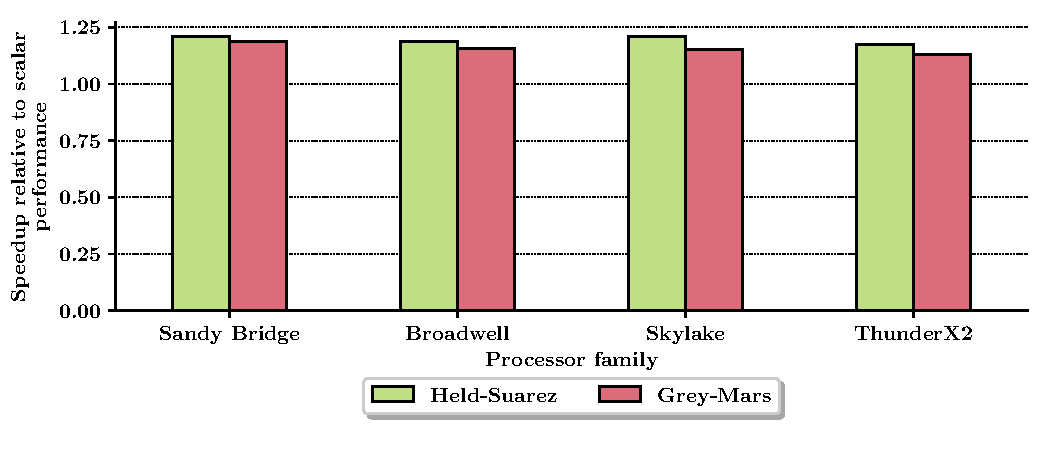
\includegraphics[width=\textwidth]{img/speedup-vector-sp.pdf}
\caption{Speedup of the vectorised code relative to scalar.}
\label{fig:vec-speed-sp}
\end{center}
\end{figure}
\par
When using single-precision floating point numbers, vectorisation accounts for an approximate 1.18$\times$ speedup of the scalar code (Figure \ref{fig:vec-speed-sp}). In comparison, vectorisation for double-precision floating point numbers only accounts for a 1.09 $\times$ speedup (Figure \ref{fig:vector-gains}). This indicates that vectorisation is more efficient when used on single-precision variables. Vector reports produced when compiling the code confirm this, as they show that SIMD instructions can now perform operations over complex data structures across all processor architectures, including the ThunderX2. 
\par
%For the single precision code, approximately 36\% of the program runtime was spent inside vectorised compute kernels, compared to just 28\% of runtime for the double precision code. This suggests that more loops are able to use vector instructions when using single precision variables. 

\subsection{Conclusions and discussion}
%Although Isca is not stochastic, it is chaotic, which means that small changes to variables can lead to drastically different results. 
%The use of single-precision floating point numbers produces a significant performance speedup of the model compared to the default double-precision code. This can be attributed to the reduction of resource usage such as 
\par
Isca is currently used to research the climate behaviour of exoplanets of which very little is known of atmospheric conditions, and therefore results of these simulations are expected to be imprecise. To account for this, Isca calculates the global means of atmospheric variables to be used as approximations, and for this use-case single-precision variables are adequate.
\par
Meteorologists typically use a brute-force approach to model parameter selection, whereby many different simulations are run with only slight variations to parameter settings. The use of single-precision variables would be useful in this situation, as more parameter configurations could be tested in the same amount of time. Parameter settings that produce interesting results can be rerun using double-precision variables at a higher resolution. 

\subsection{Verification of results}
In the Fortran 90 standard, single-precision real numbers have 7 digits of accuracy, and double-precision real numbers have 15 digits of accuracy. Because of this, the units of last place numerical analysis technique cannot be used to compare single and double-precision outputs. To verify the scientific validity of the results, both single and double-precision output files were given to domain experts for comparison. 

\section{FFTW with single-precision variables}

\subsection{Performance analysis}

\subsubsection{Methodology}
The wallclock runtime of the code using both optimisations was measured and compared against optimisations $A$, $B$ and the unmodified code. FFTW provides both a double and single-precision version of its library, so it remains compatible with Isca when compiled to use single-precision variables by default.
\subsubsection{Results}
\begin{figure}[H]
\begin{center}
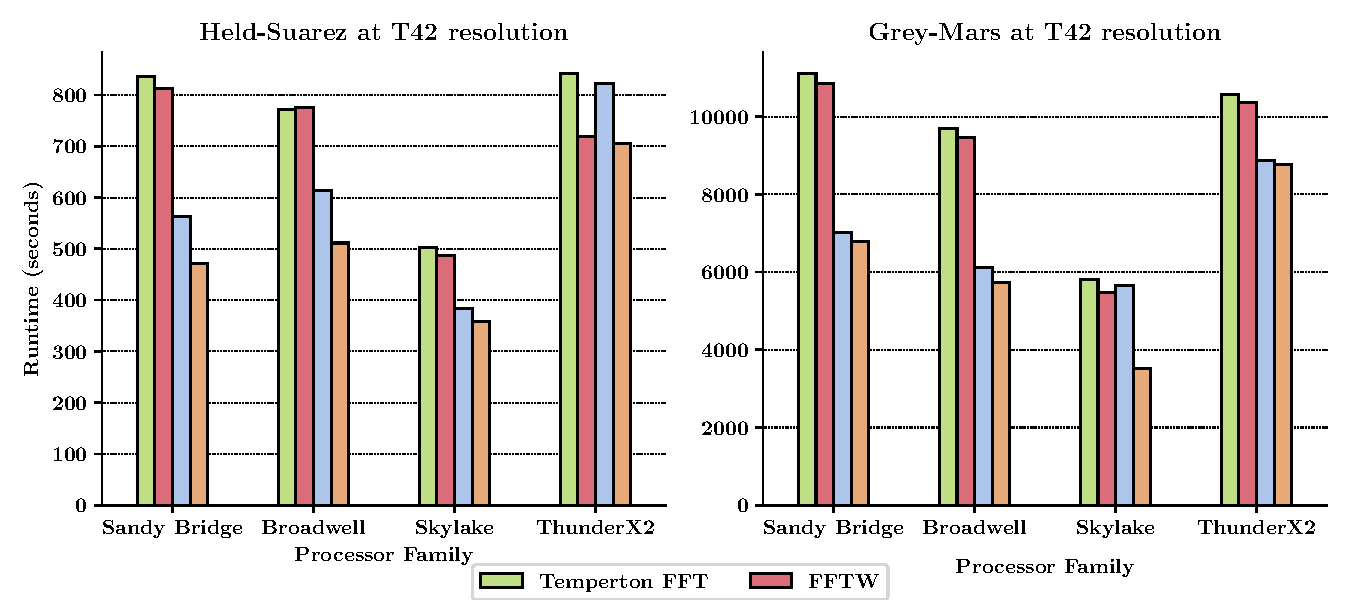
\includegraphics[width=\textwidth]{img/opt_comparison.pdf}
\caption[Runtimes of all optimisations]{Performance comparison of the Held-Suarez and Grey-Mars configuration at T42 resolution when using different performance optimisations.}
\label{fig:opt-comparison}
\end{center}
\end{figure}

\begin{figure}[H]
\begin{center}
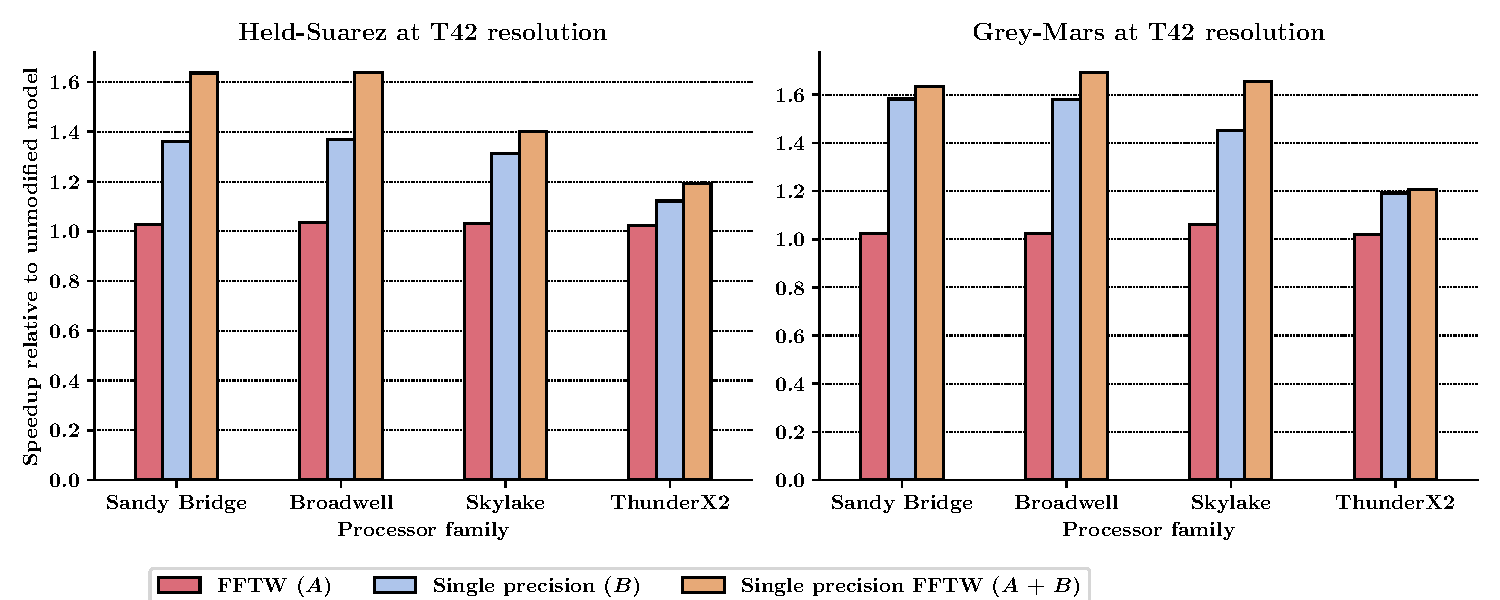
\includegraphics[width=\textwidth]{img/speedup-opt.pdf}
\caption{Speedup of performance optimisations relative to the unmodified model.}
\label{fig:opt-comparison}
\end{center}
\end{figure}


The Skylake node provided the best overall performance for the fully optimised model, with a mean wallclock runtime of 358.8 seconds for the Held-Suarez configuration, and 3,515.7 seconds for the Grey-Mars configuration  (Figure \ref{fig:opt-comparison}). These runtimes correspond to a speedup of 1.40$\times$ and 1.65$\times$ relative to the unoptimised code, respectively.  The ThunderX2 presents the worst performance, providing a mean wallclock runtime of 705.7 seconds for the Held-Suarez configuration and 8,776.4 seconds for the Grey-Mars configuration. It also provided the smallest performance speedup of 1.19$\times$ and 1.20$\times$ the unoptimised code for the Held-Suarez and Grey-Mars configurations, respectively. 
\par

\subsubsection{Conclusions and discussion}
%The results may be skewed as the model is only run on half of the nodes available on the ThunderX2, so this is only really a measure of half of the nodes performace. This is unavoidable due to the domain decomposition imposed by the model. 
%some stuff
The code responsible for performing the FFT in Isca only accounts for approximately 5-10\% of the total compute costs of the model, depending on the model configuration. Although FFTW runs 5$\times$ faster than Temperton's FFT in some cases, the overall performance improvement to Isca is minor. However, when the FFTW library is used together with single-precision variables there is a synergistic effect, resulting in an even greater overall performance gain then when either optimisation is used alone. 
\par

%The Intel processors deliver the best performance improvement. 


\section{Conclusions}
This chapter presented two performance optimisations, demonstrating runtimes up to 1.65$\times$ faster than the unmodified model on a Skylake node. Additionally, the findings from this chapter suggest that bespoke high-performance code does not improve over time, and that specialist libraries should be used when possible as they are usually kept up to date with modern hardware developments.
\par
Despite the improvement of the FFT, there is very little scope for optimisation without addressing the deeper rooted problem of the MPI imbalance discussed in Section \ref{sec:mpi-comms}. Although the use of single-precision floating point numbers did improve the performance of the model, this was not because of reduced communication times between processor ranks. Optimising the MPI communication would require a total redesign of the model, and may be not possible to do using a distributed-memory programming model such as MPI.

%
% Chapter performance projection
%
\chapter{Performance projection}
Using the results from the experiments carried out in Chapter \ref{chap:results}, the performance of Isca has been projected to Fujitsu's A64FX Arm processor, which is planned to be debuted in the Post-K supercomputer in 2021 \cite{yoshida2018fujitsu}. Most notably, it will be the first production processor to use the new Arm \gls{sve} instruction set architecture, which allows for SIMD operations using 512-bit vector registers. Estimating the performance of unreleased hardware is challenging as manufacturers often release optimistic performance estimations to generate interest in their devices.
\par
This chapter aims to use the literature published by Fujitsu to estimate the raw performance of of the A64FX processor. This information is then used to project the performance of Isca to the A64FX using a simple performance model based on Amdhal's law \cite{bach2015est}.

\section{Hardware performance estimation}


\begin{table}[htp]
\caption{Hardware comparison of the Cavium ThunderX2 and Fujitsu's A64FX. As the A64FX is under development, this information is subject to change.}
\begin{center}
\begin{tabular}{lcc}
\toprule
\textbf{Feature} 					& \textbf{ThunderX2} & \textbf{A64FX}	\\ \midrule
Instruction set architecture (base)		& Armv8.1			& Armv8.2-A		\\
Instruction set architecture (extension) 	& NEON			& SVE			\\
Number of cores 					& 32				& 48 + 4			\\
SIMD width (bits)					& 128			& 512			\\
Floating point performance (GFLOPS)	& 537.6			& 2,688			\\
Memory bandwidth (GB/s)				& 240			& 1024			\\


\bottomrule


\end{tabular}
\end{center}
\label{table:armcomp}
\end{table}%

\subsection{Floating point performance}
Using Equation \ref{equ:perf}, a dual socket configuration of the A64FX is calculated to provide a theoretical peak floating point performance of 2,688 GFLOPS, which is a 2,150.4 GFLOP improvement over the ThunderX2. This estimation has been calculated assuming that all operations are performed using the full width of the 512-bit vector registers, which is highly unlikely for real applications. 
\par
The A64FX is expected to have a low clock rate of between 1.7-1.9 GHz. This is much lower than the Skylake processor, which must decrease its clock speed when using its 512-bit vector registers. It is not unreasonable to assume that the A64FX will not implement dynamic frequency scaling as the base clock rate is already low. 

\subsection{Memory-bandwidth}
When announced, Fujitsu claimed that the processor will deliver a peak memory bandwidth of 1024 GB/s (Table \ref{table:armcomp}) \cite{yoshida2018fujitsu}. STREAM TRIAD results can expect to achieve 80\% of peak performance, resulting in a functional memory bandwidth of 819.2 GB/s. 

\section{Isca performance estimation}
To estimate performance of Isca on the A64FX, it is important to consider only the performance of the ThunderX2 processor, as it is the only processor tested in this study that uses the Armv8 instruction set architecture.


\subsection{Scalar estimation}
The degree to which the number of processor cores affects the runtime of a parallel code can be calculated. In 1967, Gene Amdahl proposed Amdhal's law, which governs the theoretical speedup in latency of a code when run in parallel \cite{amdahl1967validity}. It states that the theoretical speedup of a parallel task ($S$) is dominated by the fraction of the task that must run in serial ($p$). It is formally expressed in Equation \ref{equ:amdahl}.

\begin{equation}
	S(n) = \frac{1}{(1-p) + \frac{p}{n}}
	\label{equ:amdahl}
\end{equation}

To estimate performance, we first need to find the amount of speedup possible applied to the proportion of execution time that can benefit from additional compute resources $\frac{p}{n}$. This can be done using non-linear least squares regression by treating Amdhal's law as an objective function of speedup. This method calculates the parallel fraction of the code as $p = 0.9776 +/- 0.0011$.
\par
\begin{figure}[htbp]
\begin{center}
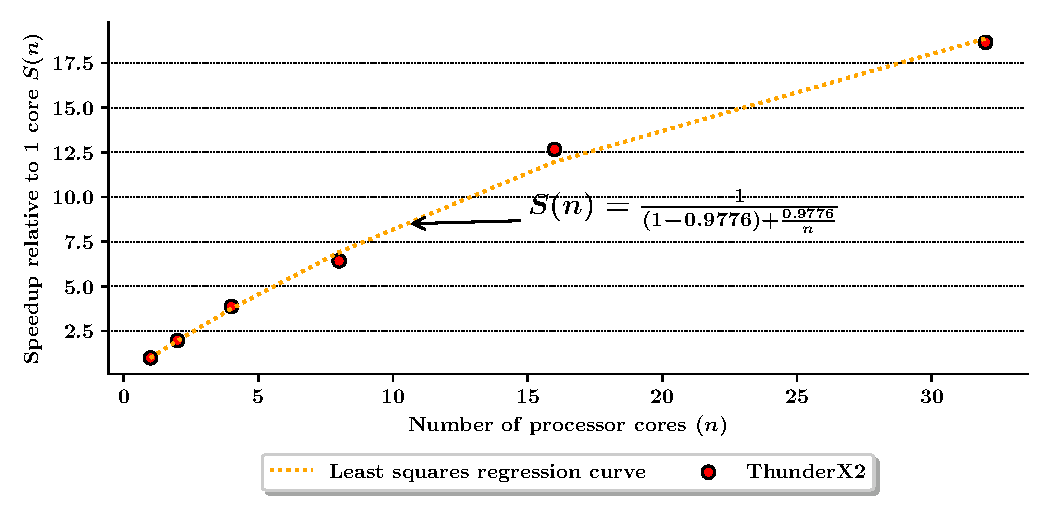
\includegraphics[width=\textwidth]{img/a64fx-estimate.pdf}
\caption[Non-linear least squares regression ]{Non-linear least squares regression applied to the speedup of the scalar ThunderX2 code relative to one processor core.}
\label{default}
\end{center}
\end{figure}

\par
To estimate the performance of a processor, the number of cores effectively utilised to run the code in parallel $e$ must be calculated using Equation \ref{equ:effective-cores}, whereby $m$ refers to the maximum number of cores on the processor.
\begin{equation}
e = \frac{1}{(1-p) + \frac{1}{m}}
\label{equ:effective-cores}
\end{equation}
\par
We then calculate the scalar floating point performance of the processor. Assuming a base clock frequency $f$ of 1.8 GHz for the A64FX, the number of floating point operations can be estimated to be 59.47 for the ThunderX2 and 59.59 for the A64FX (Equation \ref{eq:flop-est}).
\begin{equation}
G = f \cdot e
\label{eq:flop-est}
\end{equation}
\par
The wallclock runtime of the A64FX, $R_{A}$ can be estimated using the floating point performance of both the ThunderX2, $G_{T}$ and A64FX, $G_{A}$ for each core count and runtime of the ThunderX2 $R_T$ (Equation \ref{equ:fpa}).
\begin{equation}
R_{A} = \frac{G_{T}}{G_{A}} \cdot R_{T}
\label{equ:fpa}
\end{equation}

\subsection{Vector estimation}
Thus far, all calculations have used the unvectorised benchmark of the ThunderX2. The predicted wallclock runtime $R_{A}$ must be adjusted to account for the 512-bit registers found in the A64FX. On the ThunderX2, the code compiled to use SIMD is on average 1.035$\times$ faster than the scalar code. We can therefore assume that the performance gain will be twice that for a vector width of 256 bits, and quadruple that for a width of 512 bits. Consequently, we can estimate that the A64FX will see between a 1.1$\times$ and 1.2$\times$ performance gain from the use of SIMD instructions and this can be applied to scale the estimate $R_{A}$. This estimate is reasonable, as the Isca code does not heavily rely on vectorisation for performance. 

\subsection{Results}
It is estimated that Isca will run faster on the A64FX than the ThunderX2, providing an approximate 1.17$\times$ +/-10\% performance speedup relative to the ThunderX2 at all core counts (Figure \ref{fig:projection}). 
\begin{figure}[htbp]
\begin{center}
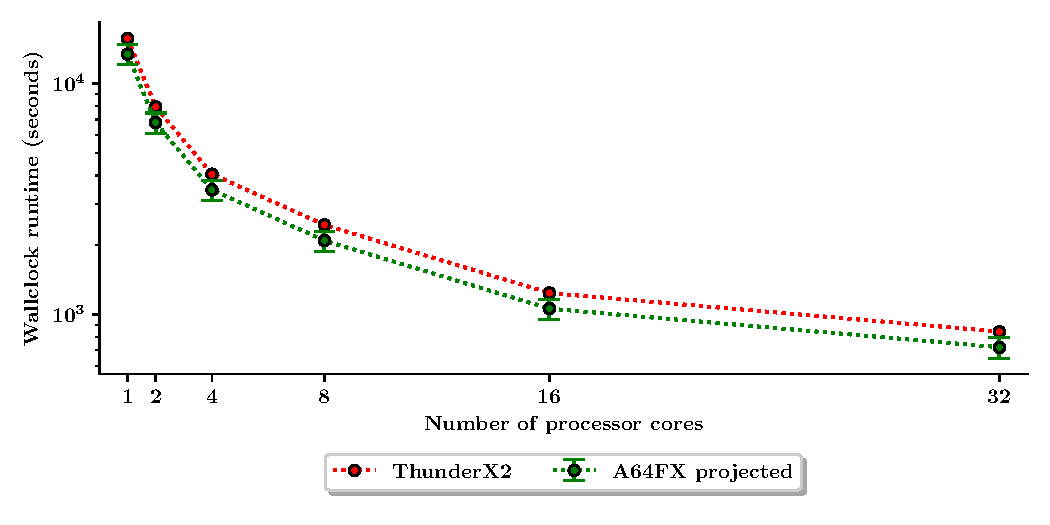
\includegraphics[width=\textwidth]{img/a64fx-projection.pdf}
\caption{Projected performance of the A64FX compared to the measured performance of the ThunderX2 running the Held-Suarez configuration at T42 resolution. }
\label{fig:projection}
\end{center}
\end{figure}





%The Held-Suarez model configuration running at T42 resolution was found to have an operational intensity of 0.11 FLOP/Byte, and a total floating point performance of 1.54 GFLOPS (Figure \ref{fig:roofline}). The T42 resolution operates over 8192 grid points, and performs calculations at a rate of 0.11 seconds per grid point per iteration. From this, we can determine that the model requires 169.4 floating point operations per grid cell. 1.54 * 0.11

\section{Conclusion}
These estimates are more of a thought experiment than a methodical performance model of the Isca code, using only the speed and estimated vector gain of the processor whilst not taking the memory-bandwidth into account. However, they provide an interesting insight into the performance of the future of Arm server hardware running a production scientific code. 


%\begin{figure}[htbp]
%\begin{center}
%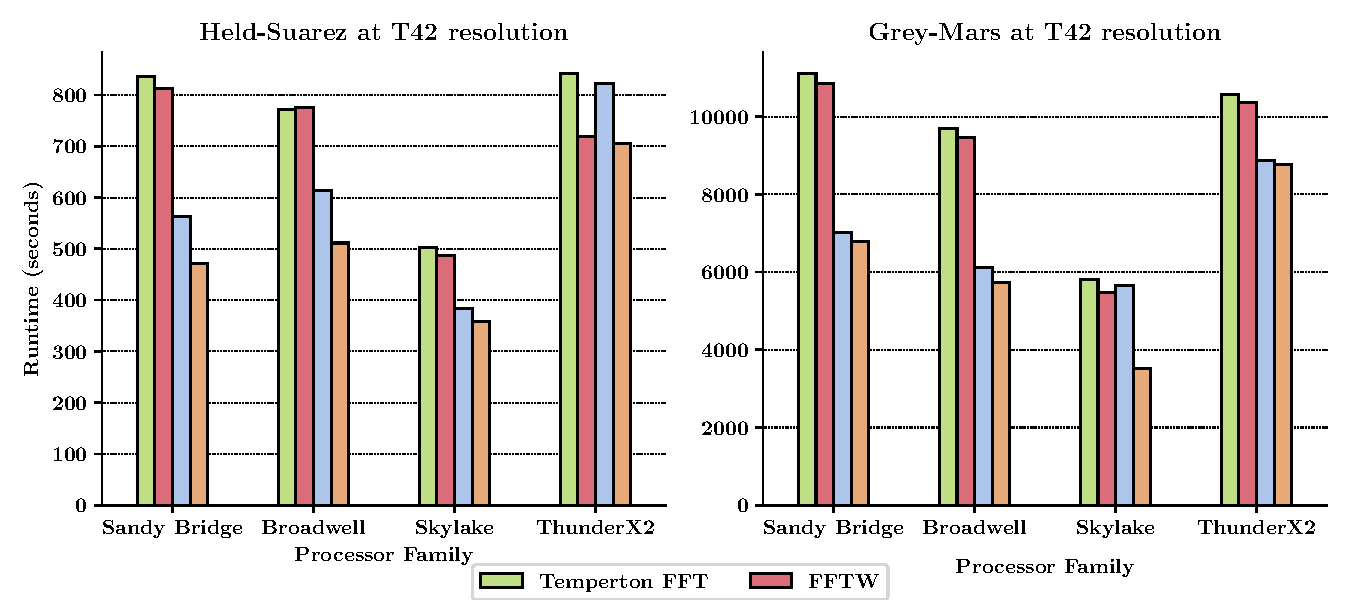
\includegraphics[width=\textwidth]{img/opt_comparison.pdf}
%\caption{default}
%\label{default}
%\end{center}
%\end{figure}




%\section{Optimisation Methodology}
%Performance bottlenecks were found using the Intel Parallel Studio Extended Edition (PSXE) on \gls{bcp3}, \gls{bcp4} and \gls{bp}; Cray Performance Analysis and Tuning (CRAYPAT) was used on Isambard. 
%
%Intel splits their toolset into multiple products, each aiming to improve code performance through different means. The Intel PSXE manual recommends that the following tools are used to identify and address performance limiting factors of the following types.
%\begin{description}
%	\item[Advisor] This tool can be used to determine why some loops are not using vector instructions, as well as counting the FLOPs within time-consuming loops. 
%	\item[VTune Amplifier] CPU/ memory bound 
%	\item[Trace Analyzer and Collector] MPI bound 
%\end{description}
%
%\url{https://software.intel.com/sites/products/snapshots/application-snapshot/}.
%
%\subsection{Intel Tools}
%
%To find optimisations, the code was profiled using X, Y and Z. 




%%% Reflection and critical analysis

\part{Reflection, Critical Evaluation and Conclusion}


\chapter{Reflection}
This chapter presents a reflection of the challenges encountered throughout the course of this research project. 

\section{The Fortran programming language}
The initial challenge was learning the Fortran programming language, having not used it prior to this project. This was complicated further by the size and complexity of the Isca codebase, which made it difficult to learn the language by example. Fortran behaves very differently from other more familiar programming languages like C and Python, and a long time was spent learning the intricacies of the language before any real development could take place. The process of learning the language involved writing many small toy programs to test the behaviour of different subroutines. 

\section{Compilation of the model}
Prior to starting this project, no performance optimisations had been identified and there was no guarantee that the code could be optimised. This placed a lot of pressure on ensuring that the model could compile and run so that the project could progress onto benchmarking, and then performance optimisation. Simply compiling the model was a non-trivial process, and it took 4 weeks before Isca could compile and run on each cluster without crashing or hanging. There were many small problems with the codebase that were unique and difficult to research, and often required an obscure fix in the form of a compiler flag or environment variable. Using a range of compilers generated further problems, as different compilers caused the code to produce unique behaviours.
\par
At the beginning of the project, a large amount of time was spent on compiling the model using CCE on the Isambard supercomputer. When tested, the executable produced by this compiler provided worse performance than GCC and was therefore not used throughout the rest of the project. With hindsight, this time may have been better spent identifying other performance optimisations, or using the Arm HPC compiler instead.
\par
Isca is a very fragile codebase and even minor changes caused the model to crash. The main source of crashes throughout this project occurred as a result of atmospheric variables exceeding their expected range. The chaotic nature of the model meant that this was a frequent occurrence, as small changes to parameter values would cause vastly different results. Isca can sometimes take up to half an hour to compile, especially when using the CCE compiler. This proved to be challenging when implementing code changes, as minor mistakes sometimes required a total recompilation of the model, wasting a significant amount of development time. 
\par
Much of the FMS code does not strictly follow the Fortran standard, and relies heavily on compiler features that exist only to remain compatible with legacy codes.
\par
Many issues occurred on the BluePebble supercomputer as the cluster was still in its beta phase of development throughout the duration of this project. Many of the fixes could not be performed by changes to the codebase, and required cooperation with the system administrators to change the configuration of the PBS module. One issue unique to this machine was caused by the overuse of stack memory, which resulted in segmentation faults when running the model at higher resolutions. Upon initialisation, Isca sets the amount of stack memory it requires, however BluePebble does not grant permissions to its users to allow for this to be done.

\section{Data collection}
The Python library written for data collection was invaluable as the volume of test runs that were required to collect accurate data would have been unmanageable to perform manually. Even when using this library, a large portion of all jobs submitted failed for various reasons. At the beginning of the project, it was a common occurrence for 9 out of 10 submitted jobs to fail. However as the project progressed, each cluster and configuration used its own submission script, so that the correct resources could be requested for each configuration. Although some jobs would still crash, this greatly reduced the rate of failure.
\par
Additionally, the Python library allowed for the collected data to be visualised in the various graphs shown throughout this document. All trends and behaviours of the code were identified from the visualisation of data. 


\chapter{Critical evaluation and conclusion}
This project aimed to present a comprehensive performance analysis and optimisation of the Isca climate model on multiple processor architectures. The following chapter assesses whether this has been achieved and discusses the limitations of the work presented. 
\par
%Isca was successfully ported to three new high performance computers using three different compilers. 

\section{Critical evaluation}

\subsection{Areas of improvement}
Although this research project presents a grounded performance analysis of numerous high-performance processors, Isca is just one program and the performance of said processors cannot be judged based on this alone. Isca also has a relatively low computational intensity for a high-performance code, and did not push any of the processors tested to their limits. More computationally intensive programs like TeaLeaf, CloverLeaf, or other synthetic benchmarking codes would provide a better platform for performance comparison, as mentioned in Section \ref{sec:cluster-bench} \cite{mcintosh2017tealeaf, mallinson2013cloverleaf}.
\par
The results presented in Chapter \ref{chap:results} may disproportionately represent the performance of the T42 resolution. The best performance of the ThunderX2 was observed at the T85 model resolution, however many of the experiments were performed at the T21 and T42 resolutions only. This may cause the ThunderX2 to be misrepresented, as the T21 and T42 resolutions could only utilise 16 and 32 out of the 64 cores available, respectively. This was unintentional, however providing benchmarks across all different combinations of processor, configuration and resolution was challenging to manage, and the T42 resolution was chosen as the default for many experiments. The time restrictions of the three-month project meant that it was simply not possible to collect results for all possible scenarios. In this project, the accuracy of results was prioritised over collecting inconsistent data for many experiments. 

%After the results had been collected for all experiments, Isca was recompiled using GCC on the ThunderX2 using the \texttt{-mtune=thunderx2t99} compiler flag. This is a hint to the compiler  This improved the performance of the code by approximately 7\% however it was too late in the project to recollect all of the results for this processor.

\subsection{Conclusion}
Whilst considering the scale of this project, the results support other evidence that indicates that the ThunderX2 processor delivers competitive levels of performance to that of modern Intel processors \cite{mcintosh2018performance}. The ThunderX2 gave the best level of performance when running Isca at a high resolution (T85) and the cause of this was determined to be the large core count of the processor, which allowed for communication to stay within a single node. However, it was still outperformed by the Broadwell processor when running on two nodes. 
\par
To identify performance optimisations an extensive performance analysis of the Isca climate model has been presented. The main performance-limiting factor identified is a severe load-balancing issue, which causes up to 40\% of the program runtime to be spent on blocking MPI communication. This results in a large cost for unavoidable points of synchronisation when performing global operations such as calculating means. This issue was exaggerated when running across multiple nodes, causing substandard levels of scaling for multinode configurations. 
\par
When a project is not constrained by time limits, optimisation efforts are typically focused on improving the greatest performance bottlenecks of a code \cite{asanovic2006landscape}. However, optimising the MPI in this case would be a significant feat of software engineering, requiring more time than available to three-month MSc project.
\par
Although the main performance-limiting factor could not be optimised, considerable research was undertaken to identify, design and implement an optimisation to the FFT, which was the second most time-consuming part of the code. Isca performs a spherical FFT, which constrains the type of FFT that can be used. This required an extensive review of the literature regarding FFT algorithms before the correct type of FFT was identified in the FFTW library.
\par
The outcomes of this project indicate that it has been successful. The Isca codebase has been ported to three new supercomputer clusters, one of which is now actively used by researchers at the University of Bristol. The meteorological research group at the University of Bristol has purchased a £10,000 dedicated compute node for the BluePebble supercomputer as a direct result of the work presented in this thesis. Additionally, 223 compute nodes on BCP3 and 168 compute nodes on Isambard can now be utilised by users of Isca. 


\section{Further work}
At the resolutions commonly used by Isca, the code does not scale outside of a single compute node. This raises questions as to why the model was written to use MPI, instead of a shared-memory programming model such as OpenMP. When the FMS was under development in the 1990s, compute nodes typically consisted of only one or two processor cores, which means that large scale MIMD parallelism would only be possible using MPI. As the number of processor cores per node have increased, perhaps an OpenMP port of the code would be viable. Although this would not completely remove the need for points of synchronisation, it would negate the cost of operations like global broadcasts, which could be executed without direct message passing. 
\par
The work presented in this thesis measured spatial resolutions up to and including T85 only. Isca officially supports resolutions up to T170, however it would be trivial to modify the Python library to allow for simulations of arbitrary granularity. Larger resolutions would allow for the model to be run across 10s of nodes rather than just the maximum of three used in this project. Although this is non-standard and does not represent how the model is used by researchers, it would be interesting to study how the model responds to greater levels of parallelism. However, the results of this project suggest that the additional cost of communication would outweigh the benefits of additional parallelism. Higher resolutions would also allow for the ThunderX2 processor to be tested in a multinode configuration, which was not investigated as part of this study. 
\par
The performance of Isca could be measured relative to the performance of other climate modelling codes. The current literature provides some benchmarks of other climate models running the Held-Suarez model configuration, however these studies have been performed on vastly different hardware from that used in this thesis, and therefore cannot be used for a direct comparison of the model \cite{schmidt2007benchmark}. Further work could compare the runtime of other climate models such as the Unified Model on the same hardware as used in this project.
\par
Although this research project focussed solely on porting and optimising the Isca climate model, working on the code for an extended period of time has revealed some shortcomings of the software architecture. The Python wrapper used to run the model and handle data collection is used only as a scripting language to repeatedly run a Fortran executable. This means that multiple versions of the same model configuration cannot exist concurrently, as only one executable can exist for a single model configuration at any time. A more user-friendly design would be to encapsulate the entire model in a Python program, replacing the \texttt{main} Fortran entry point with a Python script. This script would makes calls to Fortran routines using F2PY, instead of just using Python as a scripting language to run the model \cite{peterson2009f2py}. This may sacrifice some performance, however many Python libraries are now written in compiled languages like C, C++ or Fortran, and offer the performance benefits of these languages whilst retaining the usability of Python. This change to the codebase would allow for greater customisation of model configurations, as well as allowing for multiple concurrent versions of the model to exist at the same time. 
\par
Although the Grey-Mars and Held-Suarez model configurations are vastly different, they only represent two narrow use-cases of the Isca model. Isca can be used for the simulation of countless other scenarios, ranging from the benignly simple to complex realistic global simulations. Further work could look at other use-cases included in the Isca Github repository, including a `hot Jupiter', `bucket hydrology' and realistic Earth simulation using topography \cite{isca2019github}. 
\par
Unpredictable behaviour was observed on the Sandy Bridge compute nodes (BCP3), whereby there were large fluctuations in the runtime of simulation epochs, and internode communication times were much larger than single node times. Whilst some interpretation of this has been explored, no definitive cause was identified.
\par
Hewlett Packard Enterprise in collaboration with Arm, SUSE, and the Universities of Bristol, Edinburgh and Leicester have worked together to produce the Catalyst supercomputer. This machine consists of three identical clusters situated at each university, each consisting of 64 Hewlett Packard Apollo 70 systems, containing two 32 core Cavium ThunderX2 processors. As Isca has demonstrated compelling performance on the Isambard supercomputer, it could be ported to and run on Catalyst. 







%\begin{itemize}
	%\item It was difficult to find things to optimise. The biggest time-sink was the MPI, but that was due to unavoidable load-balancing issues that cannot be resolved through asynchronous message passing. 
	%\item Prior to starting the project, there was no guarantee that the code could be optimised in any way. A lot of time was spent looking for stuff to optimise. 
	%\item I spent a long time at the beginning of the project getting the code to work with the Cray compiler. This was maybe a waste of time. 
	%\item I had never used Fortran before, and it was difficult to learn the language with such a massive code base. The codebase contains over 250,000 lines of code and a considerable amount of time was spent getting familiar with the different parts. 
	%\item Couldn't do 3 runs for all test cases as there simply wasn't enough time. The model compiles into a special directory, and this means that only one model can be tested at one time. 
	%\item Code crashes all the time because it's very delicate. 
	%\item Although the Python library helped, it was still very difficult to coordinate all the testing as there were many experiments to do.
%	\item Only benchmarked one code, therefore can't be a good reflection of the ThunderX2
%	\item What do the results mean? 
%	\item The codebase takes a long time to compile. The Cray compiler can take upwards of half an hour to compile the Grey-mars configuration. Sometimes a single code change can take half an hour to check if it works. 
%	\item As the number of cores per processor increases there is less point in using MPI for smaller codes like Isca. Perhaps this was unavoidable 20 years ago when processors commonly had only 1/2 cores per node but this is not the case anymore. Especially at low resolutions
%	\item there is a flag that makes the code so much faster on Isambard, but only found out 1 week before deadline so couldn't use 
%	\item Wrong programming model, perhaps Openmp would have been better, -> thinking of legacy code, Isca would have been run on nodes with only 1-2 processors on them. 
	
%	\item rewrite the model to use more Python.
%\end{itemize}



% Bibliography
\bibliographystyle{ieeetr}
\addcontentsline{toc}{chapter}{Bibliography}
\bibliography{citations.bib}

\appendix
\chapter{Porting code changes}
\label{apdx:porting}
Appendix A lists some of the code changes made in order to compile and run Isca using the Intel, GNU and Cray compilers. 
\section*{Isambard}
\subsection*{Problem 1}
\subsubsection*{Error}
This issue was caused by a variation of the Fortran standard between the Cray, GNU and Intel compilers. GNU and Intel allow for implicit conversion between logical, integer and real variables, but the Cray compiler does not. To resolve this issue, a new macro was defined to set a default value depending on the type of variables it was being used for. 
\begin{lstlisting}
ftn-356 crayftn: ERROR MPP_DO_GLOBAL_FIELD2D_L8_3D, File = mpp_do_global_field.h, Line = 123, Column = 12   Assignment of a INTEGER expression to a LOGICAL variable is not allowed.
\end{lstlisting}

\subsubsection*{Fix}
If \texttt{MPP\_TYPE\_} is of type integer or real, then 
\begin{lstlisting}[language=Fortran]
#define MPP_DEFAULT_VALUE_ 0
\end{lstlisting}
\par
If \texttt{MPP\_TYPE\_} is of type complex, then 
\begin{lstlisting}
#define MPP_DEFAULT_VALUE_ .false.
\end{lstlisting}

\subsection*{Error 2}

\begin{lstlisting}
ftn-1725 crayftn: ERROR COMPUTE_LC1, File = ../../../lustre/home/br-glancaster/Isca/src/atmos_spectral/init/polvani_2007.F90, Line = 356, Column = 26 
  Unexpected syntax while parsing the assignment statement : "operand" was expected but found "-".
\end{lstlisting}
Cray Fortran requires brackets around all values denoted as negative, for example
\begin{lstlisting}[language=Fortran]
Tr = T0 + lapse/(zt**-alpha + z(k)**-alpha)**(1./alpha)
\end{lstlisting}
becomes 
\begin{lstlisting}[language=Fortran]
Tr = T0 + lapse/(zt** (-alpha) + z(k)** (-alpha))**(1./alpha)
\end{lstlisting}

\section*{Error 3}



\chapter{Code listings}
\label{apdx:codelisting}

\section*{Grid to Fourier subroutine}

\begin{lstlisting}[language=Fortran,caption={Code used to perform an FFT using the FFTW library. This subroutine can be found in the new \texttt{fftw.F90} module, and transforms a 2D data structure from the spacial domain to frequency domain.}]
subroutine grid_to_fourier_double_2d_fftw(num, leng, lenc, grid, fourier)

integer(kind=4),            intent(in)    :: num    
integer(kind=4),            intent(in)    :: leng   
real(C_DOUBLE),             intent(in)    :: grid(leng, num)
complex(C_DOUBLE_COMPLEX),  intent(out)   :: fourier(lenc, num)
real                                      :: fact 
integer                                   :: i, j

fact = 1.0 / (leng - 1)

do j = 1, num
  do i = 1, leng - 1
    real_input(i) = grid(i,j)
  enddo

  call dfftw_execute_dft_r2c(real_input_pointer, real_input, complex_output)

  do i = 1, lenc
    fourier(i, j) = complex_output(i) * fact
  enddo
enddo
return
end subroutine grid_to_fourier_double_2d_fftw
\end{lstlisting}


\section*{Program to time FFT}
\begin{lstlisting}[language=Fortran]
subroutine time_fft()
use fft_mod

real(kind=8)   , allocatable 	:: ain(:,:), aout(:,:)
complex(kind=8), allocatable 	:: four(:,:)
integer 	:: i, j, m, n, k, h, iter, lot
integer 	:: ntrans(3) = (/ 128, 256, 512 /)
integer 	:: lots(3) = (/ 64, 128, 256 /)
real 	    :: start_time = 0, stop_time = 0, mean_time_iter = 0, mean_time_full = 0, append_time = 0, time_3d_start = 0, time_3d_stop = 0

iter = 100

! test multiple transform lengths
  do m = 1, 3

  ! set up input data
    n = ntrans(m)
    lot = lots(m)

    allocate(ain(n+1,lot),aout(n+1,lot),four(n/2+1,lot))

    call fft_init(n)

    do k = 1, iter
        call random_number(ain(1:n,:))
        four = fft_grid_to_fourier(ain)
        call cpu_time(start_time)
            aout = fft_fourier_to_grid(four)
        call cpu_time(stop_time)
        append_time = append_time + (stop_time - start_time)
    enddo

    mean_time_iter = append_time / iter

    append_time = 0.0
    start_time = 0.0
    stop_time = 0.0

    do k = 1, iter
        call random_number(ain(1:n,:))
        four = fft_grid_to_fourier(ain)
        call cpu_time(time_3d_start)
        do h = 1, 25
            aout = fft_fourier_to_grid(four)
        enddo
        call cpu_time(time_3d_stop)
        append_time = append_time + (time_3d_stop - time_3d_start)
    enddo

    mean_time_full = append_time / iter

    call fft_end()
    deallocate (ain,aout,four)

    print *, '( ',n,' x ' ,lot ,' ), mean_iteration_time: '
    write (*,'(f15.9)') mean_time_iter
    print *, '( ',n,' x ' ,lot ,' ), mean_full_time: '
    write (*,'(f15.9)') mean_time_full
 enddo

end subroutine time_fft

end program test
\end{lstlisting}


\chapter{Compile environment scripts}
\label{apdx:compile-env}

\section*{Isambard GNU}

\begin{lstlisting}[language=Bash]
# template for the  gfortran compiler
# typical use with mkmf
# mkmf -t template.ifc -c"-Duse_libMPI -Duse_netCDF" path_names /usr/local/include
CPPFLAGS = -I/usr/local/include
NETCDF_LIBS = `nf-config --fflags  --flibs`

# FFLAGS:
#  -cpp: Use the fortran preprocessor
#  -ffree-line-length-none -fno-range-check: Allow arbitrarily long lines
#  -fcray-pointer: Cray pointers don't alias other variables.
#  -ftz: Denormal numbers are flushed to zero.
#  -assume byterecl: Specifies the units for the OPEN statement as bytes.
#  -shared-intel:  Load intel libraries dynamically
#  -i4: 4 byte integers
#  -fdefault-real-8: 8 byte reals (compatability for some parts of GFDL code)
#  -fdefault-double-8: 8 byte doubles (compat. with RRTM)
#  -O2: Level 2 speed optimisations

FFLAGS = $(CPPFLAGS) $(NETCDF_LIBS) -cpp -fcray-pointer \
          -O2 -ffree-line-length-none -fno-range-check \
          -fbacktrace -target-cpu=arm-thunderx2 -fdefault-real-8 -fdefault-double-8

#         -ftree-vectorize -fopt-info-vec-missed

#FFLAGS = $(CPPFLAGS) $(NETCDF_LIBS) -cpp -fcray-pointer \
#          -O2 -ffree-line-length-none -fno-range-check \
#          -fdefault-real-8 -fdefault-double-8 -fbacktrace \
#              -target-cpu=arm-thunderx2 

FC = $(F90)
LD = $(F90) $(NETCDF_LIBS)

LDFLAGS = -lnetcdff -lnetcdf 
CFLAGS = -D__IFC
\end{lstlisting}

\section*{BCP3 Intel}
\begin{lstlisting}[language=Bash]
# template for the Intel fortran compiler
# typical use with mkmf
# mkmf -t template.ifc -c"-Duse_libMPI -Duse_netCDF" path_names /usr/local/include
CPPFLAGS = -I/usr/local/include
NETCDF_LIBS = `nc-config --libs`

# FFLAGS:
#  -fpp: Use the fortran preprocessor
#  -stack_temps:  Put temporary runtime arrays on the stack, not heap.
#  -safe_cray_ptr: Cray pointers don't alias other variables.
#  -ftz: Denormal numbers are flushed to zero.
#  -assume byterecl: Specifies the units for the OPEN statement as bytes.
#  -shared-intel:  Load intel libraries dynamically
#  -i4: 4 byte integers
#  -r8: 8 byte reals
#  -g: Generate symbolic debugging info in code
#  -O2: Level 2 speed optimisations
#  -diag-disable 6843:
#       This suppresses the warning: `warning #6843: A dummy argument with an explicit INTENT(OUT) declaration is not given an explicit value.` of which
#       there are a lot of instances in the GFDL codebase.
FFLAGS = $(CPPFLAGS) -fpp -stack_temps -safe_cray_ptr -ftz -assume byterecl -shared-intel -i4 -r8 -g -O2 -diag-disable 6843
#FFLAGS = $(CPPFLAGS) -fltconsistency -stack_temps -safe_cray_ptr -ftz -shared-intel -assume byterecl -g -O0 -i4 -r8 -check -warn -warn noerrors -debug variable_locations -inline_debug_info -traceback
FC = $(F90)
LD = $(F90) $(NETCDF_LIBS)
#CC = mpicc

LDFLAGS = -lnetcdff -lnetcdf -lmpi -shared-intel
CFLAGS = -D__IFC
\end{lstlisting}



\chapter{Job submission scripts}
\label{apx:submission}

\section*{BCP3 (PBS)}
\begin{lstlisting}[language=Bash]
#!/bin/sh

#PBS -n held_suarez_benchmarking
#PBS -V # export all environment variables to the batch job.
#PBS -d . # set working directory to .
#PBS -q long # submit to the long queue
#PBS -l nodes=1:ppn=16 
#PBS -l walltime=72:00:00 # Maximum wall time for the
#PBS -m e -M qv18258@bristol.ac.uk 

source activate isca_env
python $BENCHMARK_ISCA/src/main.py -codebase grey_mars -mincores 4 -maxcores 4 -r T21 -r T42 -r T85
\end{lstlisting}

\section*{BluePebble (PBS Pro)}
\begin{lstlisting}[language=Bash]
#!/bin/sh
#PBS -l select=1:ncpus=28:mem=20GB
#PBS -l walltime=72:00:00

module load tools/git/2.22.0
source activate isca_env
python $BENCHMARK_ISCA/src/main.py -mincores 16 -maxcores 16 -r T21 -r T42 -codebase grey_mars -fc kind_4
\end{lstlisting}



\section*{Isambard (PBS Pro)}
\begin{lstlisting}[language=Bash]
#!/bin/sh

#PBS -q arm
#PBS -l select=1:ncpus=64
#PBS -l walltime=23:00:00
#PBS -M =qv18258@bristol.ac.uk

source ~/isca_env/bin/activate
python $BENCHMARK_ISCA/src/main.py -mincores 4 -maxcores 4 -r T21 -r T42 -r T85 -codebase held_suarez -fc cray_temp
\end{lstlisting}

\section*{BCP4 (SLURM)}

\begin{lstlisting}[language=Bash]
#!/bin/Bash

#SBATCH --job-name=benchmark_held_suarez_two_cores
#SBATCH --partition=cpu
#SBATCH --time=4-00:00:00
#SBATCH --nodes=1
#SBATCH --ntasks-per-node=24
#number of cpus (cores) per task (process)
#SBATCH --cpus-per-task=1
#SBATCH --output=held_suarez_two_cores_%j.o
#SBATCH --mail-type=ALL
#SBATCH --mail-user=qv18258@bristol.ac.uk

echo Running on host `hostname`
echo Time is `date`
echo Directory is `pwd`

module purge
source $HOME/.Bashrc
source $GFDL_BASE/src/extra/env/bristol-bc4
source activate isca_env

$HOME/.conda/envs/isca_env/bin/python $BENCHMARK_ISCA/src/main.py -mincores 2 -maxcores 2 -r T21 -r T42 -codebase held_suarez -fc gcc
\end{lstlisting}




\end{document}
